\documentclass[12pt, a4paper, simple]{eskdtext}

\usepackage{env}
\usepackage{hyperref}
\usepackage{_sty/gpi_lst}
\usepackage{_sty/gpi_toc}
\usepackage{_sty/gpi_p}
\usepackage{_sty/gpi_t}

% Код
\def \gpiDocTypeNum {81}
\def \gpiDocVer {00}
\def \gpiCode {\gpiLetterI\gpieLetterII\gpiLetterIII.\gpiStudentGroupName\gpiStudentGroupNum.\gpiStudentCard-0\gpiDocNum~\gpiDocTypeNum~\gpiDocVer}

\def \gpiDocTopic {ПОЯСНИТЕЛЬНАЯ ЗАПИСКА}

% Графа 1 (наименование изделия/документа)
\ESKDcolumnI {\ESKDfontIII \gpiTopic \\ \gpiDocTopic}

% Графа 2 (обозначение документа)
\ESKDsignature {\gpiCode}

% Графа 4 (литералы)
\ESKDcolumnIVfI {\gpiLetterI}
\ESKDcolumnIVfII {\gpieLetterII}
\ESKDcolumnIVfIII {\gpiLetterIII}

% Графа 9 (наименование или различительный индекс предприятия) задает команда
\ESKDcolumnIX {\gpiDepartment}

% Графа 11 (фамилии лиц, подписывающих документ) задают команды
\ESKDcolumnXIfI {\gpiStudentSurname}
\ESKDcolumnXIfII {\gpiTeacherSurname}
\ESKDcolumnXIfV {\gpiTeacherSurname}

\begin{document}
    \begin{ESKDtitlePage}
    \begin{center}
        \gpiMinEdu \\
        \gpiEdu \\
        \gpiKaf \\
    \end{center}

    \vfill

    \begin{center}
        \gpiTopic \\
    \end{center}

    \vfill

    \begin{center}
        \textbf{ПОЯСНИТЕЛЬНАЯ ЗАПИСКА К КУРСОВОЙ РАБОТЕ} \\
        ПО ДИСЦИПЛИНЕ <<\gpiDiscipline>> \\
    \end{center}

    \vfill

    \begin{center}
        \gpiCode \\
        Листов \pageref{LastPage} \\
    \end{center}

    \vfill

    \begin{flushright}
        \begin{minipage}[t]{.49\textwidth}
            \begin{minipage}[t]{.75\textwidth}
                \begin{flushright}
                    Руководитель

                    Выполнил

                    Консультант

                    по ЕСПД
                \end{flushright}
            \end{minipage}
        \end{minipage}
        \begin{minipage}[t]{.49\textwidth}
            \begin{flushright}
                \begin{minipage}[t]{.75\textwidth}
                    \gpiTeacherName~\gpiTeacherSurname

                    \gpiStudentName~\gpiStudentSurname

                    \hspace{0pt}

                    \gpiTeacherName~\gpiTeacherSurname

                \end{minipage}
            \end{flushright}
            
        \end{minipage}
    \end{flushright}

    \vfill

    \begin{center}
        \ESKDtheYear
    \end{center}
\end{ESKDtitlePage}
                           % Титульный лист
    % ТЗ
\ESKDthisStyle{empty}
Здесь лист с ТЗ.
\newpage
\ESKDthisStyle{formII}

\tableofcontents                                
\paragraph{Приложение А. Схема программы}
\paragraph{Приложение Б. Текст программы}
\newpage
                      % Содержание
    \newpage

\section*{Введение} % Секция без номера
\addcontentsline{toc}{section}{Введение} % Добавить в содержание

В современном мире человеку приходится сталкиваться с огромными массивами однородной информации.
Эту информацию необходимо упорядочить каким-либо образом, обработать однотипными методами
и в результате получить сводные данные или разыскать в массе конкретную информацию.
Этой цели служат базы данных.

База данных — это организованная структура, предназначенная для хранения,
изменения и обработки взаимосвязанной информации, преимущественно больших объемов.

Использование баз данных имеет ряд преимуществ:

\begin{enumerate}
    \item компактность - информация хранится в БД, нет необходимости хранить
    многотомные бумажные картотеки;
    \item скорость - скорость обработки информации (поиск, внесение изменений)
    компьютером намного выше ручной обработки;
    \item низкие трудозатраты - нет необходимости в утомительной ручной работе над данными;
    \item применимость - всегда доступна свежая информация.
\end{enumerate}

На сегодняшний день применение баз данных приобрело весьма важное значение для многих организаций,
которые для упрощения своей работы применяют компьютерные технологии.

Основная цель работы - создание веб приложения, предоставляющего пользователю инструменты для работы
с массивом структурированных данных, содержащем в себе информацию о товарах.

В современном мире программисту приходится сталкиваться с огромным количеством информации,
которую необходимо сохранить.
Хранение информации - это ее запись во вспомогательные запоминающие устройства на различных носителях
для последующего использования.
Хранение является одной из основных операций, осуществляемых над информацией,
и главным способом обеспечения ее доступности в течение определенного промежутка времени.

Информационная система (ИС) - система, предназначенная для хранения, поиска и обработки информации,
и соответствующие организационные ресурсы (человеческие, технические, финансовые и т. д.),
которые обеспечивают и распространяют информацию.

ИС предназначена для своевременного обеспечения надлежащих людей надлежащей информацией,
то есть для удовлетворения конкретных информационных потребностей в рамках определённой
предметной области, при этом результатом функционирования информационных систем является
информационная продукция - документы, информационные массивы, базы данных и информационные услуги.

Первоначально для хранения информации на ЭВМ применялись локальные массивы (или файлы),
при этом для каждой из решаемых функциональных задач создавались собственные файлы исходной
и результатной информации. Это приводило к значительному дублированию данных,
за счёт чего использовалось больше памяти вычислительной машины,
а также усложнялось обновление хранимой информации.

База данных представляет собой определенным образом структурированную совокупность данных,
совместно хранящихся и обрабатывающихся в соответствии с некоторыми правилами.
Как правило, БД моделирует некоторую предметную область или ее фрагмент.
Очень часто в качестве постоянного хранилища информации баз данных выступают файлы.

Немаловажной является и взаимосвязь информации в базе данных: изменение одной строчки
может привести к значительным изменениям других строк.
Работать с данными таким образом гораздо проще и быстрее,
чем если бы изменения касались только одного места в базе данных.

Помимо основной функции - хранения и систематизации огромного количества информации - они
позволяют быстро обрабатывать клиентские запросы и выдавать актуальную информацию.

На сегодняшний день базы данных занимают одно из первых мест для многих организаций,
которые для упрощения своей работы применяют компьютерные технологии.

Результатом разрабатываемой программы должно являться приложение,
позволяющее пользователю взаимодействовать с данными о товарах при помощи пользовательского интерфейса.

\newpage
                               % Введение
    \newpage

\section{Системны анализ и постановка задачи}

% = = = = =

\subsection{Перечень функций}

Достижение цели курсовой работы предполагает необходимость создания приложения
для работы с локальной базой данных на тему <<Товары>> с использованием пользовательского
интерфейса и решения следующих конкретных задач:

\begin{enumerate}
    \item добавление товара в базу данных;
    \item вывод товаров из базы данных;
    \item удаление товара из базы данных;
    \item изменение товара в базу данных;
    \item сохранение товаров из базы данных в файл JSON;
    \item сохранение товаров из базы данных в файл CSV;
    \item открытие файла JSON и добавление товаров в базу данных.
\end{enumerate}

% = = = = =

\subsection{Требования пользователей}

Пользовательские требования - описание на естественном языке (плюс поясняющие диаграммы) функций,
выполняемых системой, и ограничений, накладываемых на неё.

Источники: Пользователь

Документ: Пользовательские требования / требования к ПО.

Ответственный: Системный аналитик.

Эти требования должны определять только внешнее поведение системы,
избегая по возможности определения структурных характеристик системы.
Пользовательские требования должны быть написаны естественным языком с использованием
простых таблиц, а также наглядных и понятных диаграмм.

Требования пользователя к информационной системе:

Обязательные:

\begin{enumerate}
    \item должна быть реализована функция ввода данных в информационную систему;
    \item должна работать функция удаления записи из информационной системы.
\end{enumerate}

Желательные:

\begin{enumerate}
    \item информационная система должна выводить отчеты на печать.
\end{enumerate}

\newpage
 % 1. Системный анализ и постановка задачи
    \newpage

\section{Проектирование системы}

\subsection{Проектирование архитектуры ПО (модули)}

Архитектура программного обеспечения (англ. software architecture) - совокупность
важнейших решений об организации программной системы.

Архитектура включает:

\begin{itemize}
    \item выбор структурных элементов и их интерфейсов, с помощью которых составлена система,
    а также их поведения в рамках сотрудничества структурных элементов
    \item соединение выбранных элементов структуры и поведения во всё более крупные системы
    \item архитектурный стиль, который направляет всю организацию - все элементы, их интерфейсы,
    их сотрудничество и их соединение.
\end{itemize}

Документирование архитектуры программного обеспечения (ПО) упрощает процесс коммуникации
между разработчиками, позволяет зафиксировать принятые проектные решения
и предоставить информацию о них эксплуатационному персоналу системы,
повторно использовать компоненты и шаблоны проекта в других.

Архитектурный вид состоит из 2 компонентов:

\begin{enumerate}
    \item [1.] Элементы
    \item [2.] Отношения между элементами
\end{enumerate}

Архитектурные виды можно поделить на 3 основных типа:

\begin{itemize}
    \item [1.] Модульные виды (англ. module views) - показывают систему как структуру
    из различных программных блоков.
    \item [2.] Компоненты-и-коннекторы (англ. component-and-connector views) - показывают
    систему как структуру из параллельно запущенных элементов (компонентов)
    и способов их взаимодействия (коннекторов).
    \item [3.] Размещение (англ. allocation views) - показывает размещение
    элементов системы во внешних средах.
\end{itemize}

Примеры модульных видов:

Декомпозиция (англ. decomposition view) - состоит из модулей в контексте
отношения <<является подмодулем>>.

Использование (англ. uses view) - состоит из модулей в контексте
отношения <<использует>> (т.е. один модуль использует сервисы другого модуля).

Вид уровней (англ. layered view) - показывает структуру,
в которой связанные по функциональности модули объединены в группы (уровни).

Вид классов/обобщений (англ. class/generalization view) - состоит из классов,
связанные через отношения <<наследуется от>> и <<является экземпляром>>.

\subsubsection*{Иерархия модулей и подмодулей разрабатываемой программы для frontend}

Информационная система включает в себя следующие модули на frontend:

\begin{itemize}
    \item модуль не найденной страницы
    \item модуль авторизации
    \item модуль выхода
    \item модуль меню
    \begin{itemize}
        \item модуль, реализующий добавление новых записей в базу данных;
        \item модуль организации локальной базы данных с выводом информации о товарах;
        \begin{itemize}
            \item модуль удаления записи из локальной базы данных;
        \end{itemize}
        \item модуль, осуществляющий изменение записи;
        \item модуль, осуществляющий сохранение данных в JSON;
        \item модуль, осуществляющий сохранение данных в CSV;
        \item модуль, осуществляющий открытие файла JSON.
    \end{itemize}
\end{itemize}

Схема frontend модулей изображена на
\textbf{рис. \ref{fig:gpi_frontend_modules} (стр. \pageref{fig:gpi_frontend_modules})}.

\begin{figure}[!htp]
    \centering
    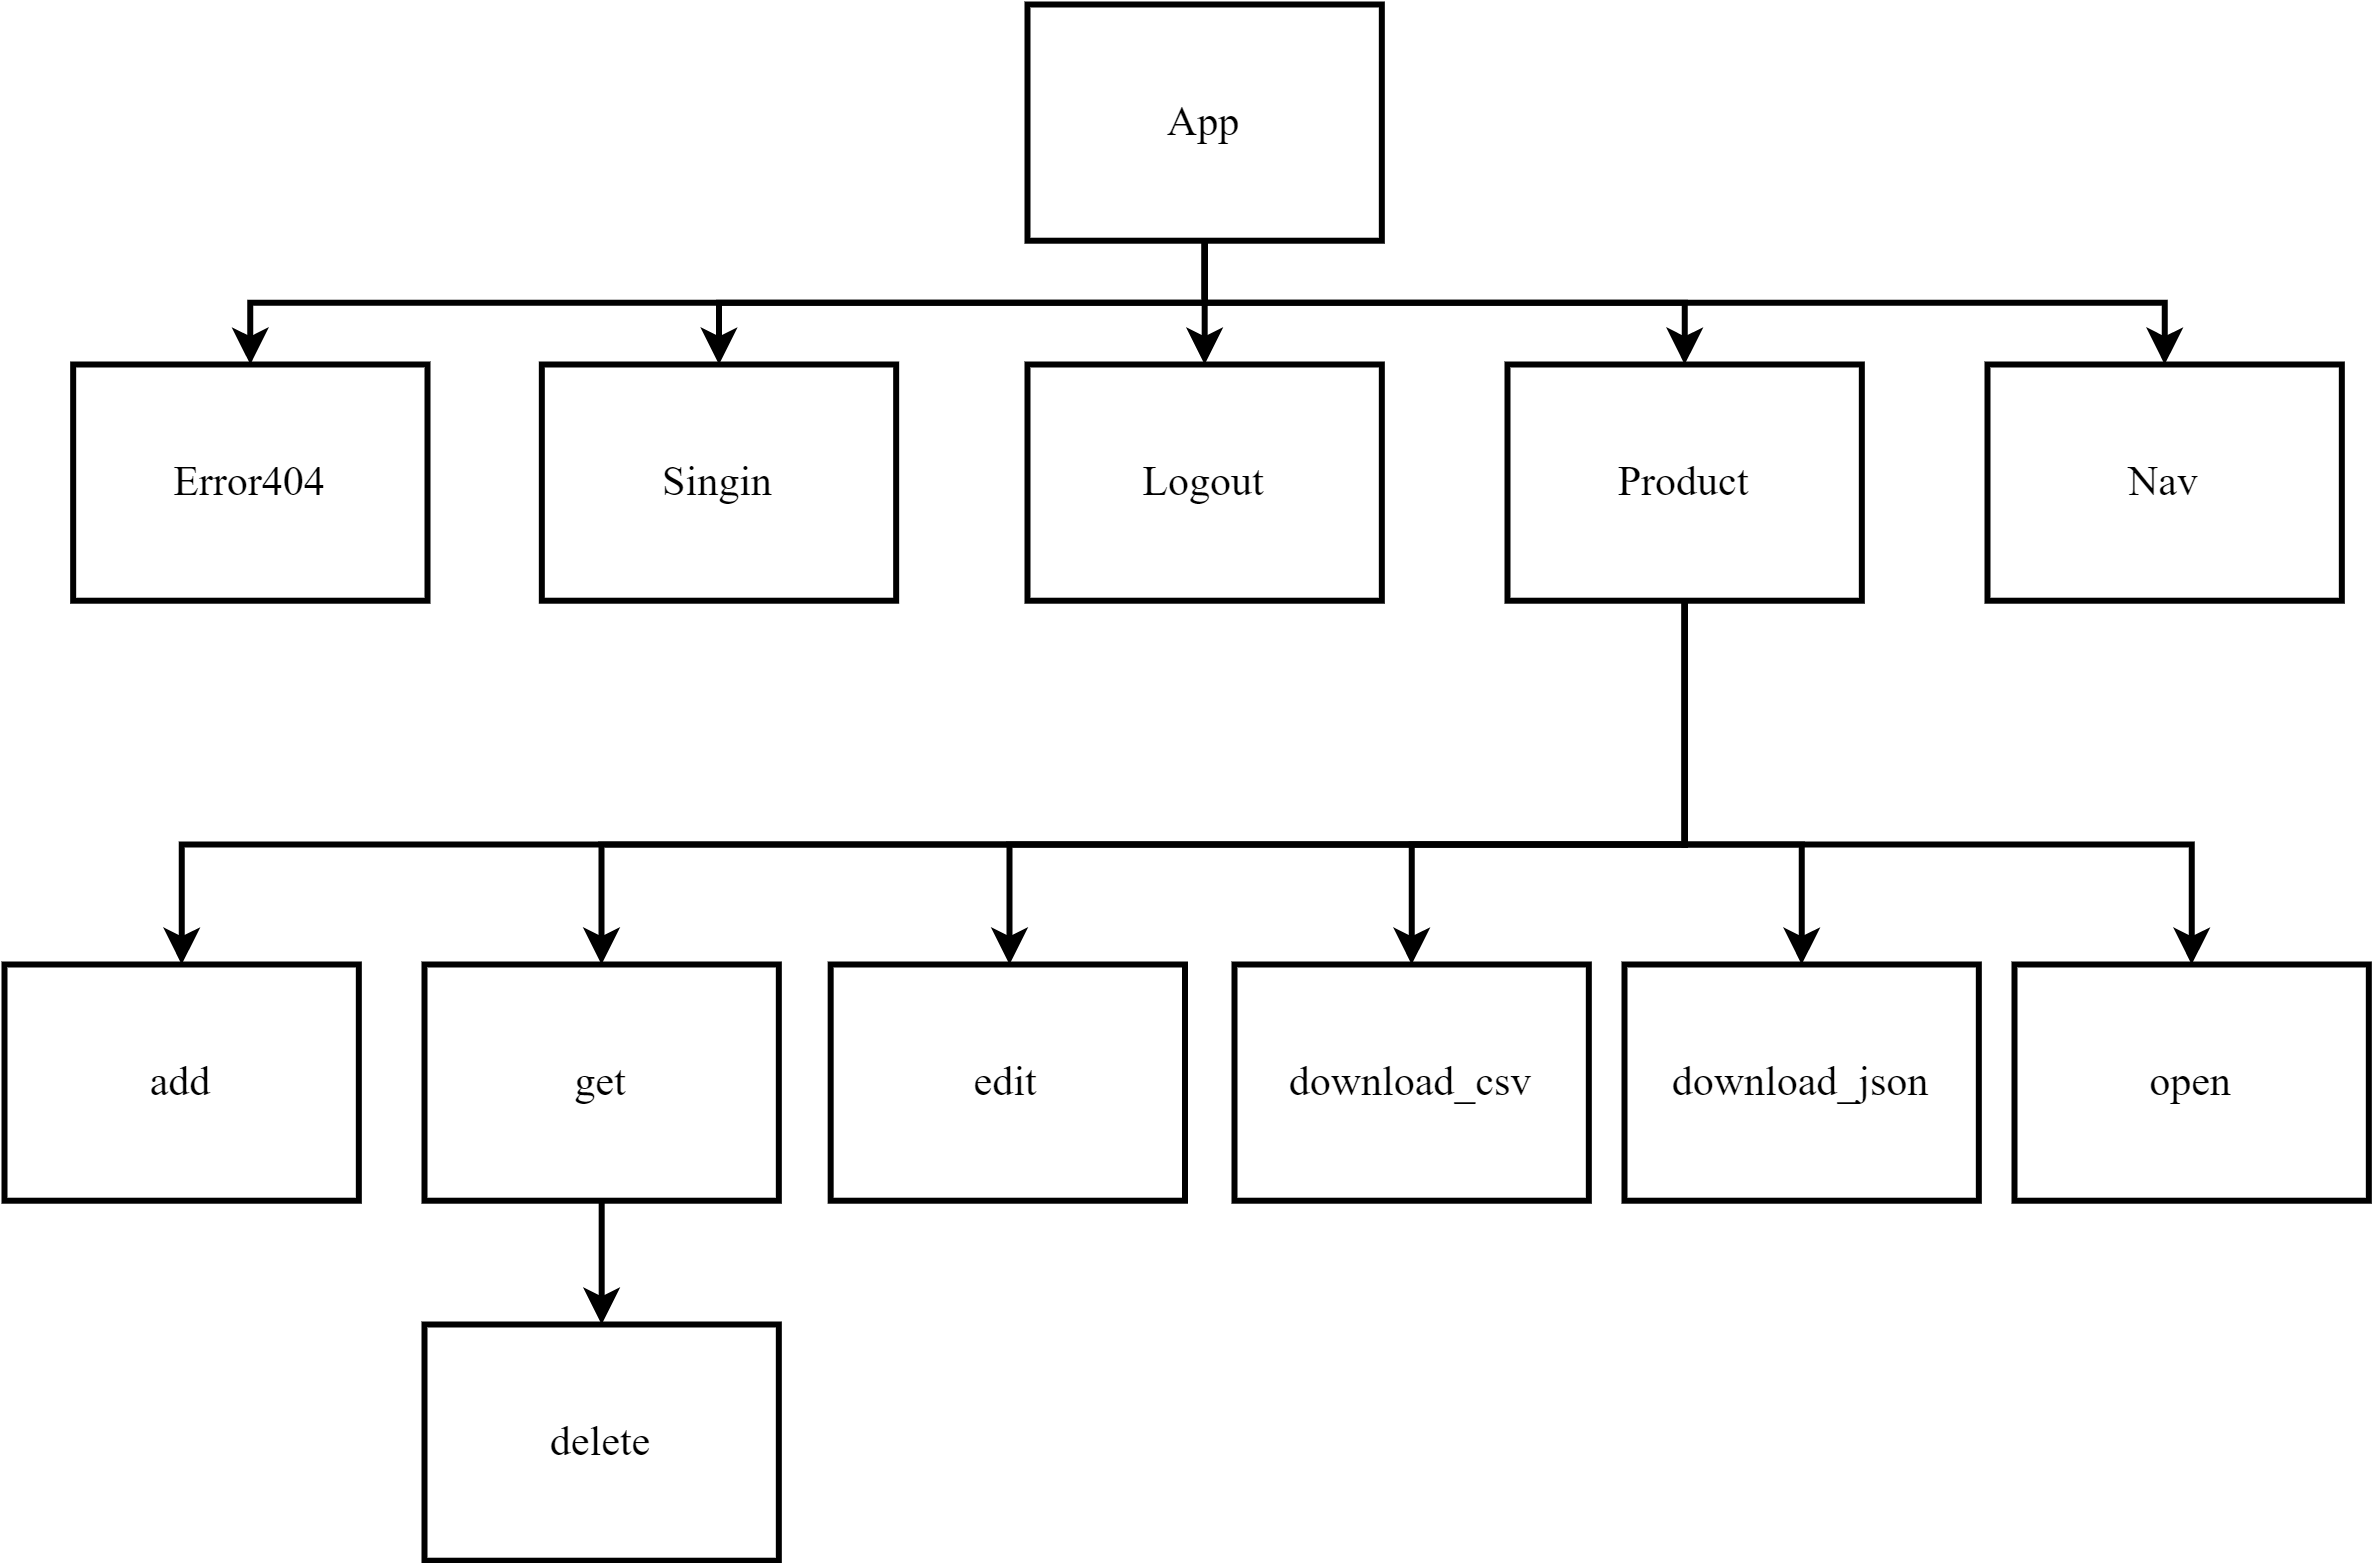
\includegraphics[width=16cm]
        {_assets/gpi_frontend_modules.png}
    \caption{Модули и подмодули для frontend}
    \label{fig:gpi_frontend_modules}
\end{figure}

\newpage

\subsubsection*{Иерархия модулей и подмодулей разрабатываемой программы для backend}

Информационная система включает в себя следующие модули на backend:

\begin{itemize}
    \item модуль авторизации;
    \item модуль добавления элементов в базу данных;
    \item модуль вывода элементов сортированных, инвертированных или по ID;
    \item модуль редактирования элемента по ID;
    \item модуль удаления элемента по ID.
\end{itemize}

Схема backend модулей изображена на
\textbf{рис. \ref{fig:gpi_backend_modules} (стр. \pageref{fig:gpi_backend_modules})}.

\begin{figure}[!htp]
    \centering
    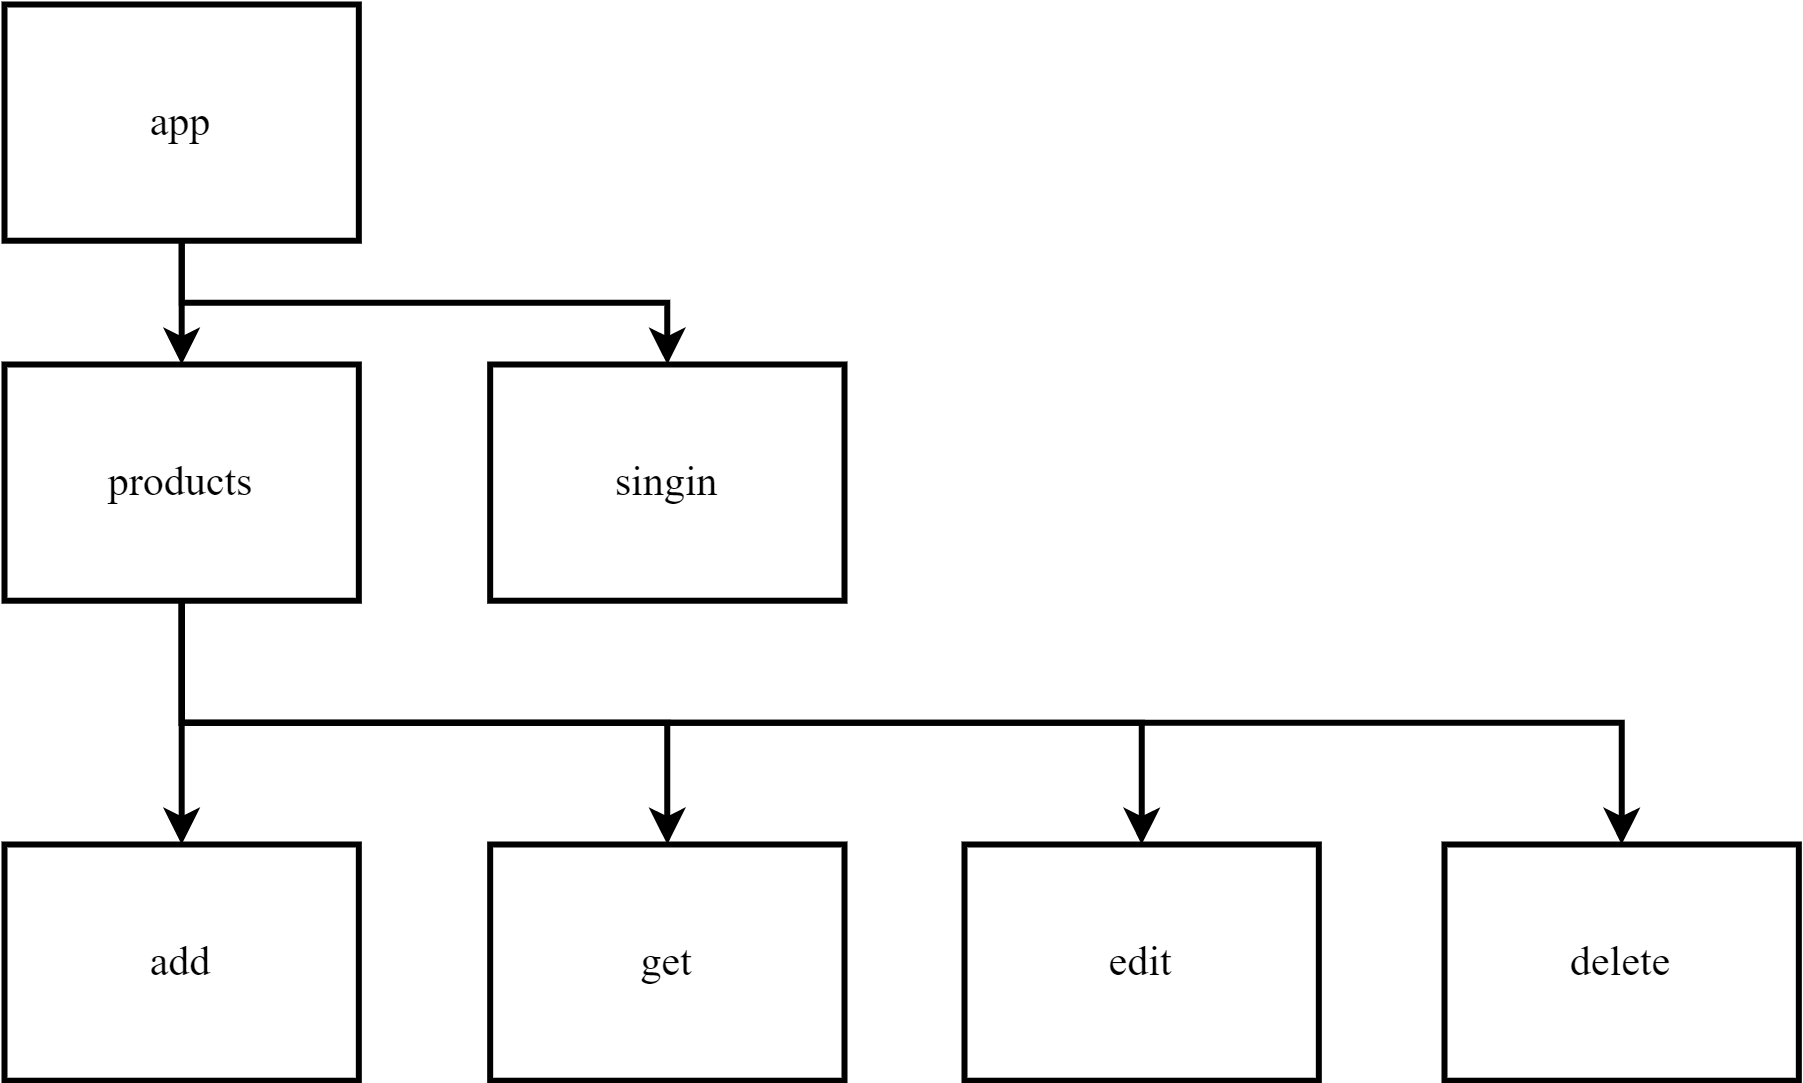
\includegraphics[width=16cm]
        {_assets/gpi_backend_modules.png}
    \caption{Модули и подмодули для backend}
    \label{fig:gpi_backend_modules}
\end{figure}

\newpage

\subsection{Проект. Схема данных}

Трёхуровневая архитектура - архитектурная модель программного комплекса,
предполагающая наличие в нём трёх компонентов: клиента, сервера приложений
(к которому подключено клиентское приложение) и сервера баз данных.

Если мы посмотрим на данную архитектуру с позиции сайта.
То первый уровень можно считать браузером (frontend), с помощью которого посетитель заходит на сайт,
второй уровень - это Express server (backend), а третий уровень - это база данных MySQL.

Схема архитуктуры ПО изображена на
\textbf{рис. \ref{fig:gpi_client_server} (стр. \pageref{fig:gpi_client_server})}.

\begin{figure}[!htp]
    \centering
    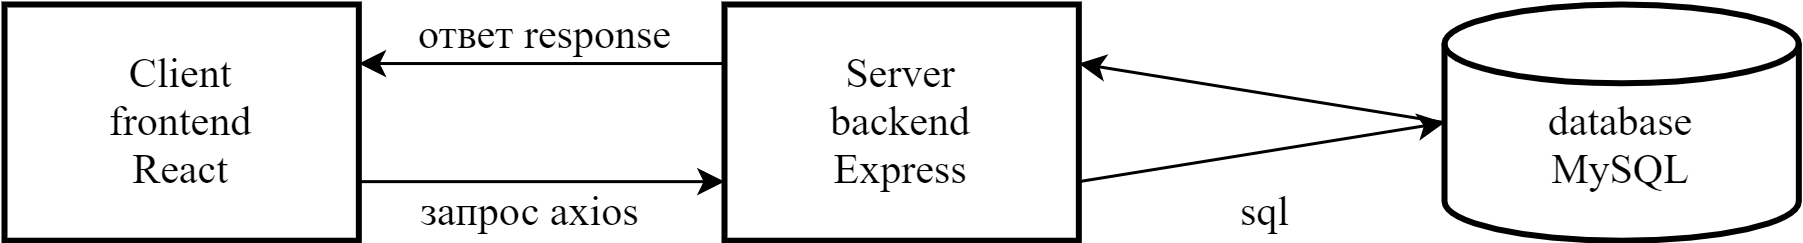
\includegraphics[width=16cm]
        {_assets/gpi_client_server.png}
    \caption{Схема архитектуры ПО}
    \label{fig:gpi_client_server}
\end{figure}

\newpage

\subsection{Проектирование UI (макеты)}

Интерфейс будет содержать шапку сайта, которая в себе содержит навигацию (основные страницы).
Макет на \textbf{рис. \ref{fig:gpi_ui_menu} (стр. \pageref{fig:gpi_ui_menu})}.

В теле сайта на странице добавления будет находится форма,
через которую можно добавить поля в базу данных.

В теле сайта на странице вывода будет таблица с элементами из базы данных.
Макет на \textbf{рис. \ref{fig:gpi_ui_get} (стр. \pageref{fig:gpi_ui_get})}.

В теле сайта на странице редактирования будет находится форма,
через которую можно изменить поля в базе данных.

В теле сайта на странице открытия файла будет кнопка загрузки файла.

В теле сайта на странице сохранения файла CSV будет кнопка загрузки файла.

В теле сайта на странице сохранения файла JSON будет кнопка загрузки файла.

\begin{figure}[!htp]
    \centering
    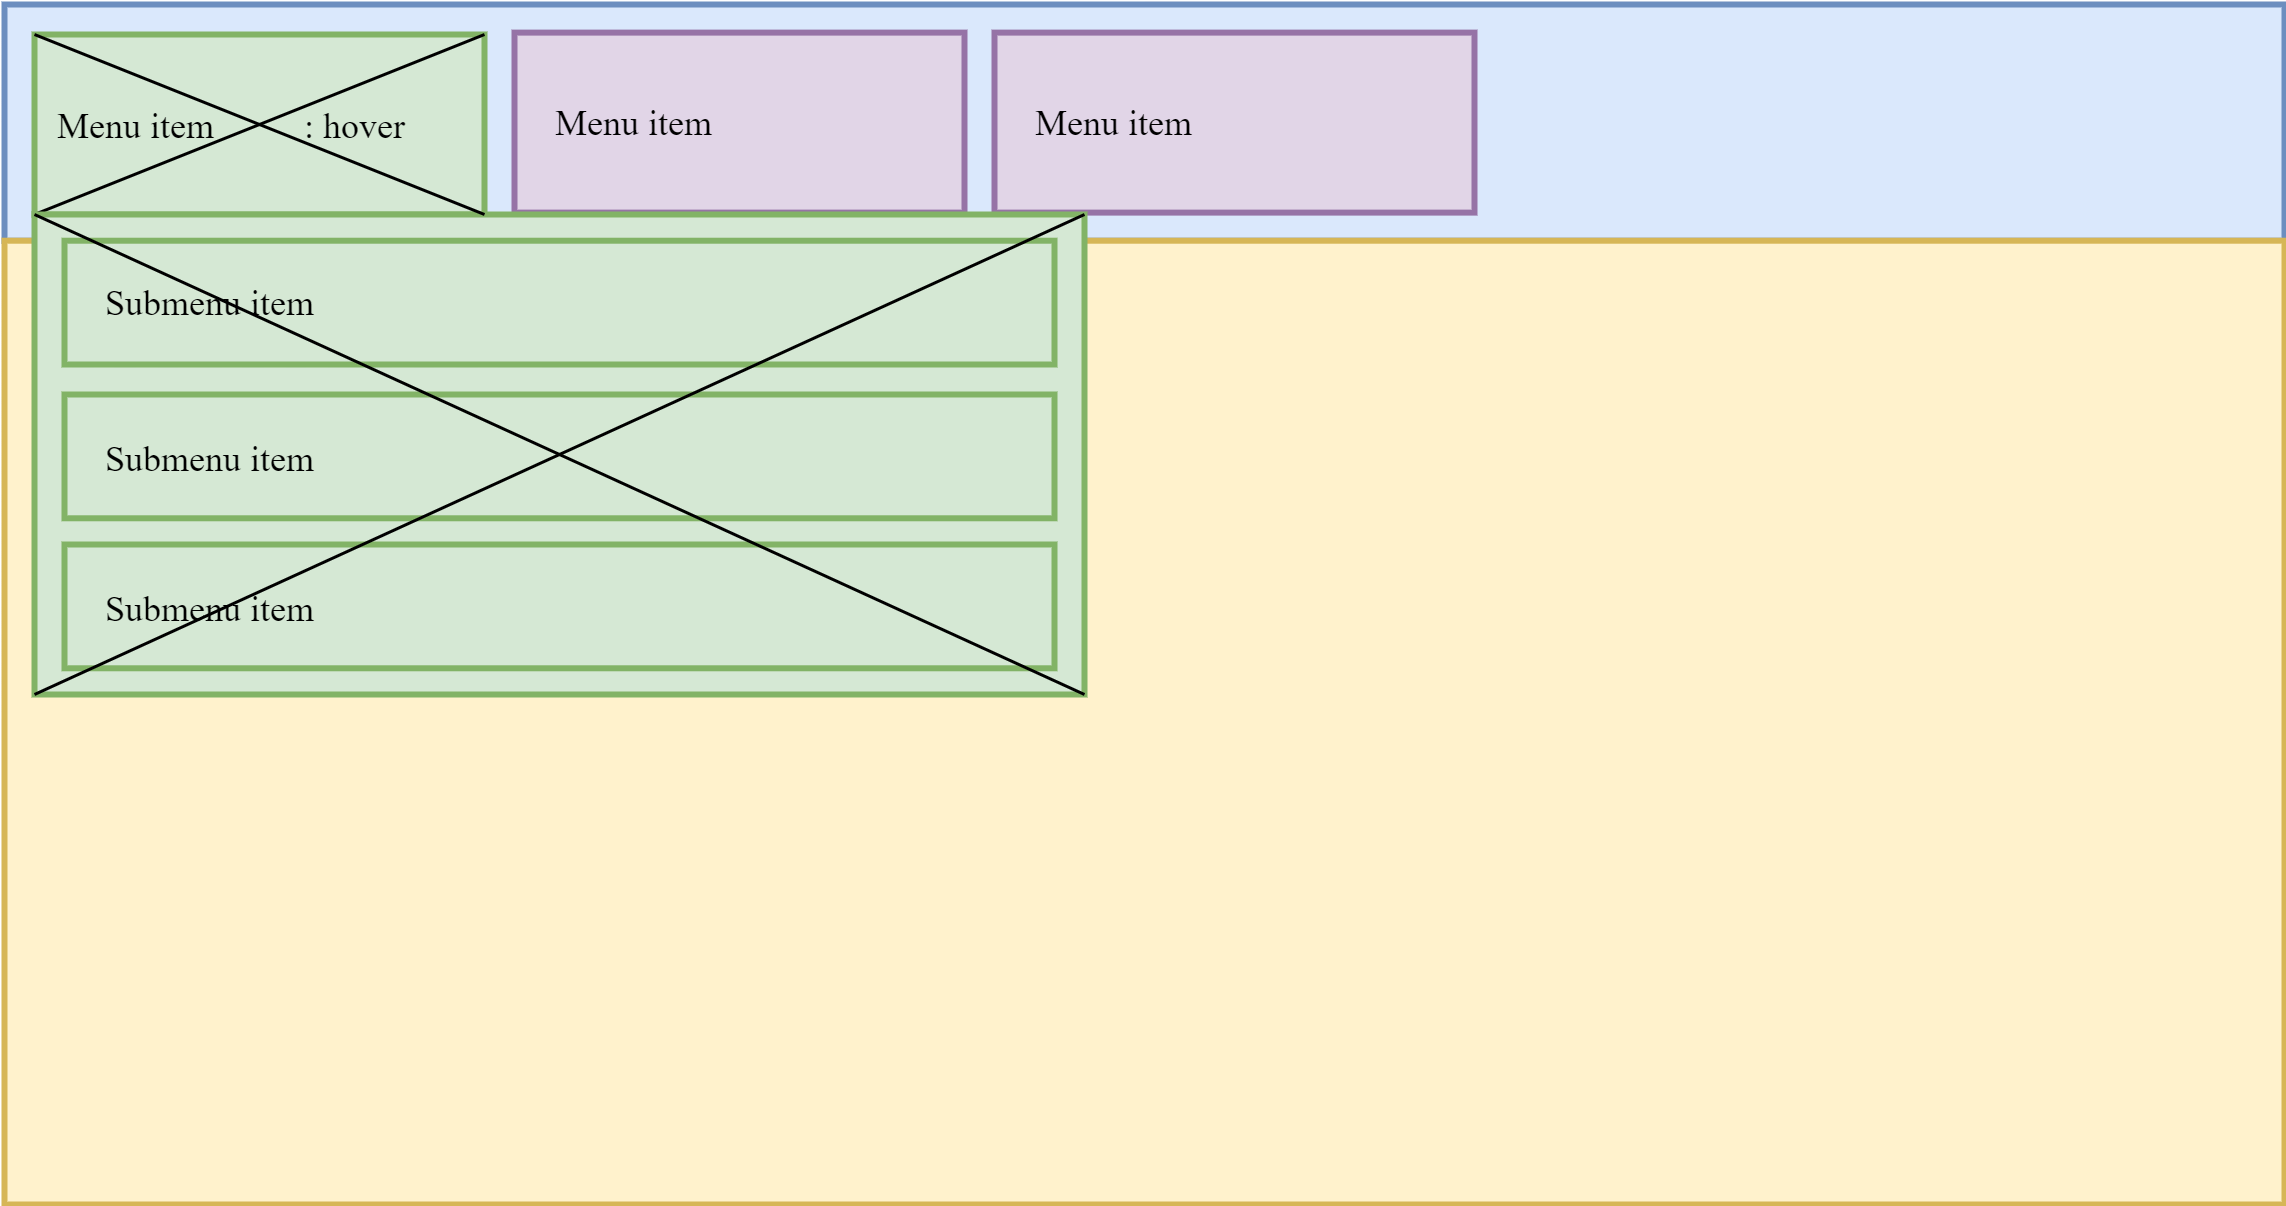
\includegraphics[width=12cm]
        {_assets/gpi_ui_menu.png}
    \caption{Макет мeню}
    \label{fig:gpi_ui_menu}
\end{figure}

\begin{figure}[!htp]
    \centering
    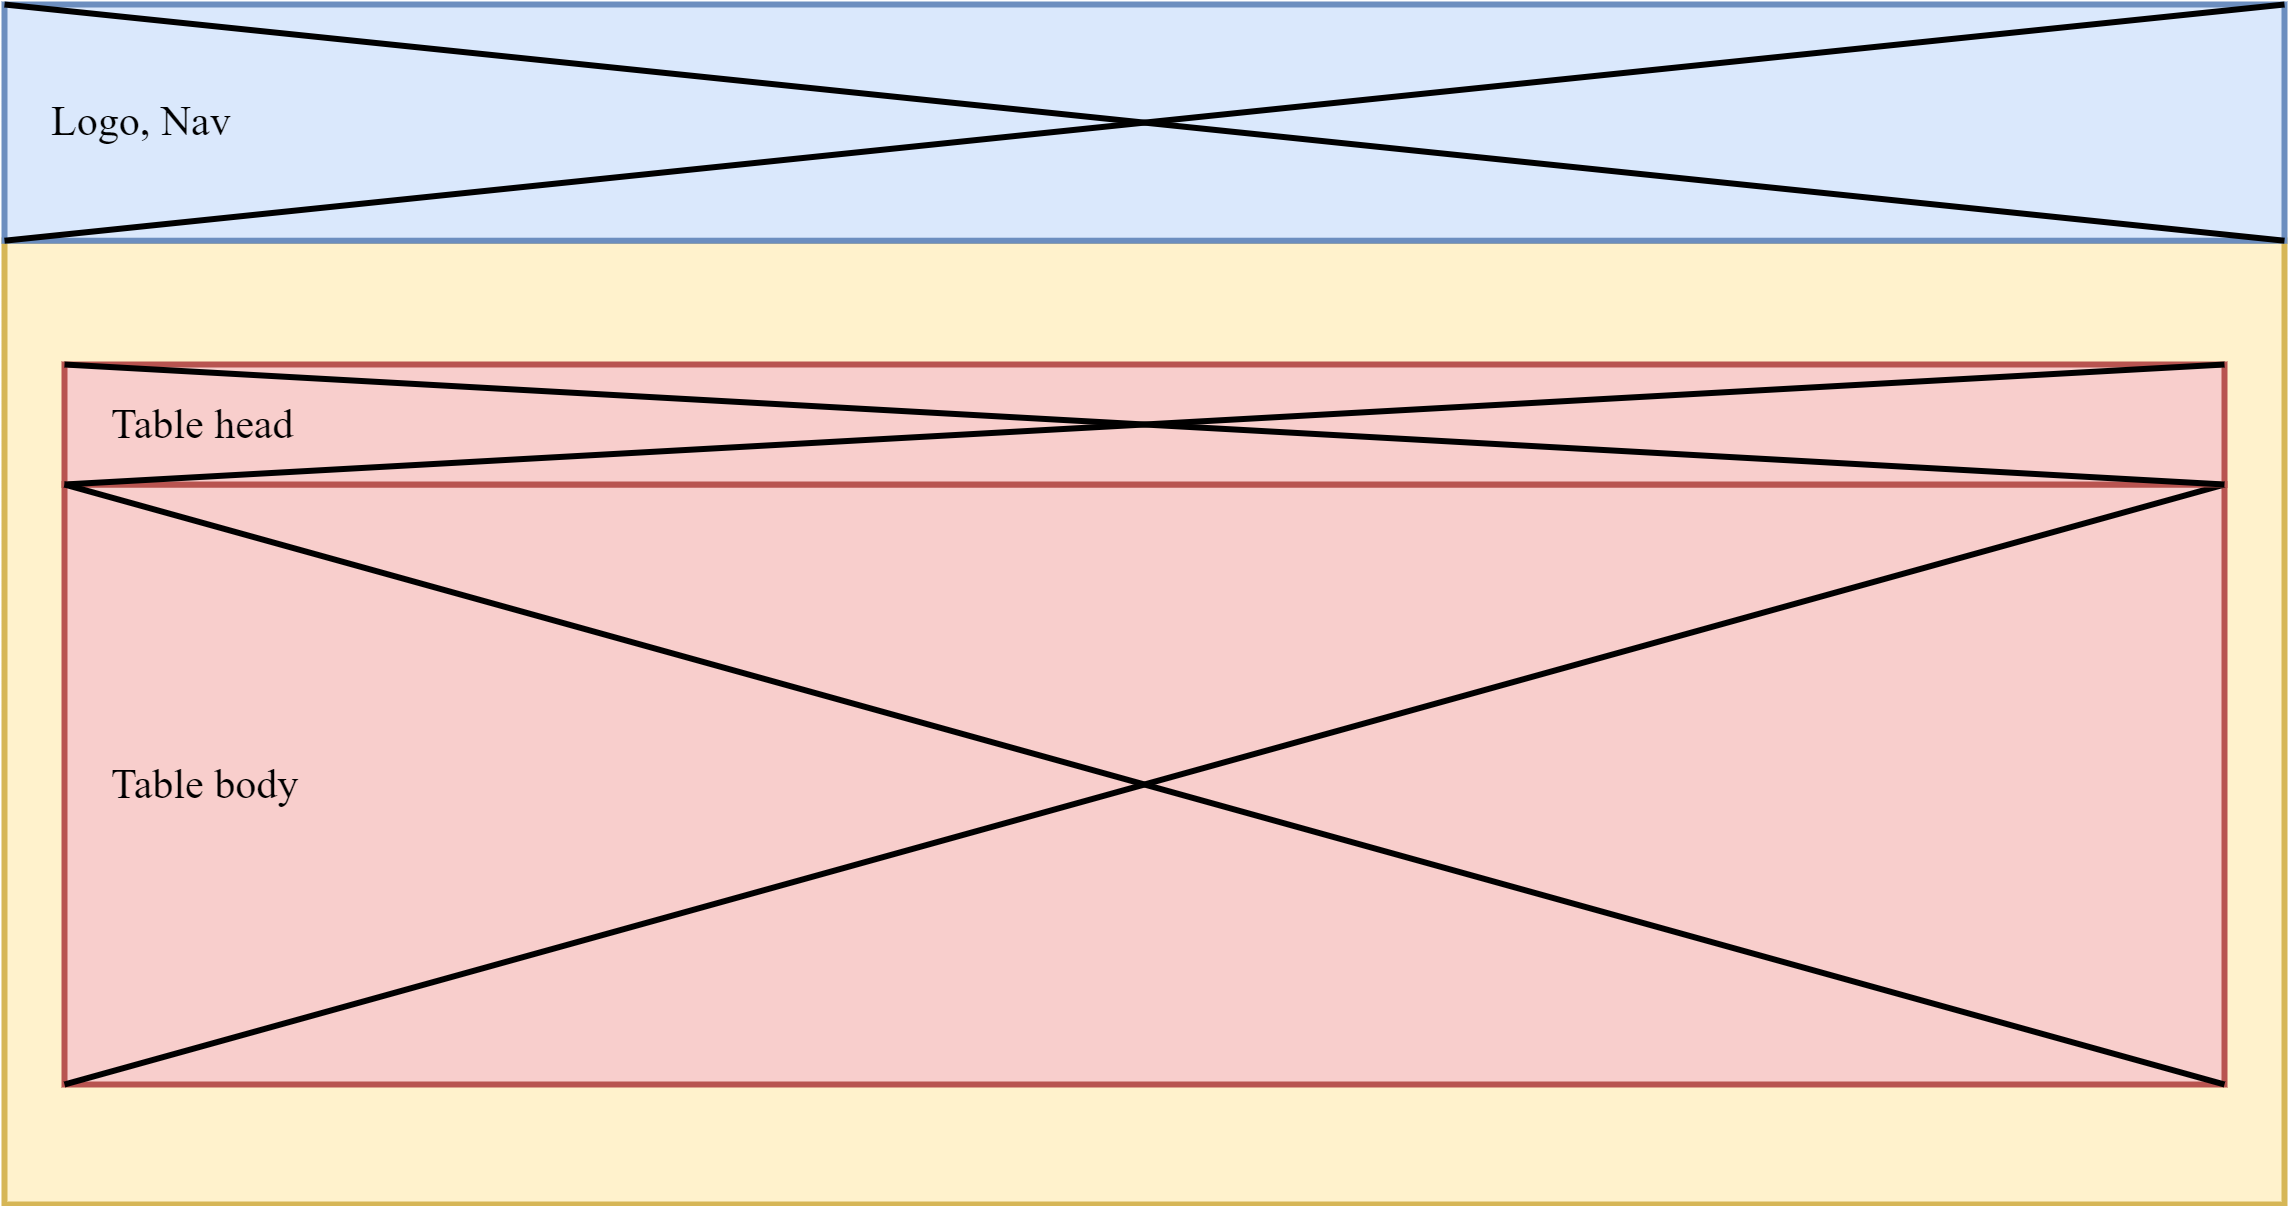
\includegraphics[width=12cm]
        {_assets/gpi_ui_get.png}
    \caption{Макет страницы}
    \label{fig:gpi_ui_get}
\end{figure}

\newpage
                      % 2. Проектирование системы
    \newpage

\section{Реализация системы}

\subsection{Докеризация}

Чтобы использовать MySQL нам нужно устанавливать LAMP (Linux, Apache, MySQL, PHP).
Это будет не удобно, если нужно будет разварачивать на нескольких компьютерах,
так как ручной ввод команд будет занимать много времени.
Чтобы автоматизировать ввод команд в курсовом проекте использовался Docker и docker-compose.

Вместо Docker и docker-compose можно было использовать решения, такие как Denwer и OpenServer,
но для этого нам нужно иметь эти программы на каждом компьютере. Имея один файл docker-compose
в проекте убивает проблему установки больших дистрибутивов, таких как OpenServer.

\subsubsection*{Установка Docker на Windows 10}

\begin{itemize}
    \item[1.] Заходим на Wikipedia и находим оффициальный сайт Docker. \\
    \url{https://ru.wikipedia.org/wiki/Docker} \\
    Находим ссылку <<Сайт docker.com>> - и переходим по ней. \\
    Скриншот на \textbf{рис.~\ref{fig:gpi_pz_docker_01} (стр. \pageref{fig:gpi_pz_docker_01})}.

    \item[2.] Открываем оффициальный сайт Docker. \\
    \url{https://www.docker.com/} \\
    Переходим на страницу загрузки, нажав на кнопку <<Get Started>>. \\
    \url{https://www.docker.com/get-started} \\
    Скриншот на \textbf{рис.~\ref{fig:gpi_pz_docker_02} (стр. \pageref{fig:gpi_pz_docker_02})}.

    \item[3.] Выбираем установщик для Windows. \\
    Скриншот на \textbf{рис.~\ref{fig:gpi_pz_docker_03} (стр. \pageref{fig:gpi_pz_docker_03})}.

    \item[4.] Запускаем установщик Windows. \\
    Скриншот на \textbf{рис.~\ref{fig:gpi_pz_docker_04} (стр. \pageref{fig:gpi_pz_docker_04})}.

    \item[5.] После установки Docker, установщик просит перезагрузить компьютер.
    Перезагружаем компьютер нажав на кнопку <<Close and restart>>. \\
    Скриншот на \textbf{рис.~\ref{fig:gpi_pz_docker_05} (стр. \pageref{fig:gpi_pz_docker_05})}.

    \item[6.] После перезагрузки компюьтера Docker автоматически запустился и просит принять лицензию.
    Соглашаемся с лицензией поставив галочку.
    Продолжаем запуск нажав на кнопку <<Accept>>.
    Скриншот на \textbf{рис.~\ref{fig:gpi_pz_docker_06} (стр. \pageref{fig:gpi_pz_docker_06})}.

    \item[7.] При запуске Docker возникает ошибка.
    Эта ошибка возникает из-за того, что у нас установлен WSL версии 1. \\
    Ошибка просит посетить сайт: \url{https://aka.ms/wsl2kernel}. \\
    Скриншот на \textbf{рис.~\ref{fig:gpi_pz_docker_07} (стр. \pageref{fig:gpi_pz_docker_07})}.

    \item[8.] По переходу по ссылке \url{https://aka.ms/wsl2kernel} происходит перенаправление
    на страницу с инструкцией об установке обновления WSL2.
    На это странице находим ссылку на загрузку установщика. \\
    Скриншот на \textbf{рис.~\ref{fig:gpi_pz_docker_08} (стр. \pageref{fig:gpi_pz_docker_08})}.

    \item[9.] Запускаем установщик. Жмём кнопку <<Next>>. \\
    Скриншот на \textbf{рис.~\ref{fig:gpi_pz_docker_09} (стр. \pageref{fig:gpi_pz_docker_09})}.
    
    \item[10.] Завершаем установку. Жмём кнопку <<Finish>>. \\
    Скриншот на \textbf{рис.~\ref{fig:gpi_pz_docker_10} (стр. \pageref{fig:gpi_pz_docker_10})}.

    \item[11.] Возврашаемся к инструкции на сайте. Эта инструкция говорит нам поменять WSL1 на WSL2,
    прописав команду в Power Shell. Копируем команду нажав на кнопку <<Copy>>. \\
    Скриншот на \textbf{рис.~\ref{fig:gpi_pz_docker_11} (стр. \pageref{fig:gpi_pz_docker_11})}.

    \item[12.] Чтобы открыть Power Shell ищем его в поиске.
    Чтобы открыть поиск зажимает клавиши <<Win>> + <<Q>>.
    В поиске прописываем <<powershell>>. Запускаем Power Shell нажав кнопку <<Open>>. \\
    Скриншот на \textbf{рис.~\ref{fig:gpi_pz_docker_12} (стр. \pageref{fig:gpi_pz_docker_12})}.

    \item[13.] Открывается Power Shell. Вставляем команду. \\
    Скриншот на \textbf{рис.~\ref{fig:gpi_pz_docker_13} (стр. \pageref{fig:gpi_pz_docker_13})}.

    \item[14.] Перезагружаем компьютер - и теперь Docker запускается без ошибки.
    Но для того, чтобы мы могли воспользоваться командами <<docker>> и <<docker-compose>>
    нам нужен какой-нибудь дистрибутив Linux. \\
    Скриншот на \textbf{рис.~\ref{fig:gpi_pz_docker_14} (стр. \pageref{fig:gpi_pz_docker_14})}.

    \item[15.] Если вернуться к инструкции, то инструкция также рекомендует нам установть
    какой-нибудь дистрибутив Linux. \\
    Скриншот на \textbf{рис.~\ref{fig:gpi_pz_docker_15} (стр. \pageref{fig:gpi_pz_docker_15})}.

    \item[16.] Нам нужен магазин приложений. Найдем его через поиск.
    Чтобы открыть поиск зажимает клавиши <<Win>> + <<Q>>.
    В поиске пишем <<Store>>.
    Открываем, нажав клавишу <<Open>>. \\
    Скриншот на \textbf{рис.~\ref{fig:gpi_pz_docker_16} (стр. \pageref{fig:gpi_pz_docker_16})}.

    \item[17.] В магизине приложении в поиске вводим <<Ubuntu>>.
    Переходим на стриницу приложения Ubuntu нажав на нужный вариант из предложенных. \\
    Скриншот на \textbf{рис.~\ref{fig:gpi_pz_docker_17} (стр. \pageref{fig:gpi_pz_docker_17})}.

    \item[18.] На странице загрузки жмём кнопку <<Get>> для того, чтобы установить приложение на компьютер. \\
    Скриншот на \textbf{рис.~\ref{fig:gpi_pz_docker_18} (стр. \pageref{fig:gpi_pz_docker_18})}.

    \item[19.] Открываем терминал Ubuntu, например, через поиск. Жмём <<Win>> + <<R>>.
    В поиске вводим <<Ubuntu>>. Жмём <<Open>>.
    При первом запуске терминала Ubuntu дистрибутив будет устанавлився.
    При установке просят придумать имя пользователя на английском. Вводим имя пользователя.
    Просят ввести пароль.
    Когда мы будет вводим вводить пароль, то символы не будут отображаться - это сделано в целях безопасности.
    Далее системы будет готова к использованию. \\ 
    Скриншот на \textbf{рис.~\ref{fig:gpi_pz_docker_19} (стр. \pageref{fig:gpi_pz_docker_19})}.
    
    \item[20.] Как уже скачали выбранный дистрибутив (в нашем случае Ubuntu),
    то в приложении <<Docker Desktop>> нужно включить наш дистрибутив.
    \begin{itemize}
        \item[1.] Запускаем <<Docker Desktop>>.
        \item[2.] Переходим в настройки нажав на шестиренку.
        \item[3.] Переходим в раздел <<Resources>>.
        \item[4.] Переходим в подпункт <<WSL INTEGRATION>>.
        \item[5.] Ставим ползунок к <<Ubuntu>>.
    \end{itemize}
    Скриншот на \textbf{рис.~\ref{fig:gpi_pz_docker_20} (стр. \pageref{fig:gpi_pz_docker_20})}.

    \item[21.] Запускаем терминал Ubuntu через поиск. Открываем поиск нажав <<Win>> + <<R>>. \\
    В поиске вводим <<Ubuntu>>. Жмём кнопку <<Open>>. \\
    Скриншот на \textbf{рис.~\ref{fig:gpi_pz_docker_21} (стр. \pageref{fig:gpi_pz_docker_21})}.

    \item[22.] В терминале Ubuntu вводим команду <<docker -v>> - и у нас выводится его версия <<Docker version 20.10.11, build dea9396>>,
    то есть у нас установлен Docker. \\
    В терминале Ubuntu вводим команду <<docker-compose -v>> - и у нас выводится его версия <<Docker Compose version v2.2.1>>,
    то есть у нас установлен docker-compose. \\
    Скриншот на \textbf{рис.~\ref{fig:gpi_pz_docker_22} (стр. \pageref{fig:gpi_pz_docker_22})}.

\end{itemize}

\begin{figure}[!p]
    \centering
    \begin{minipage}{0.47\textwidth}
        \centering
        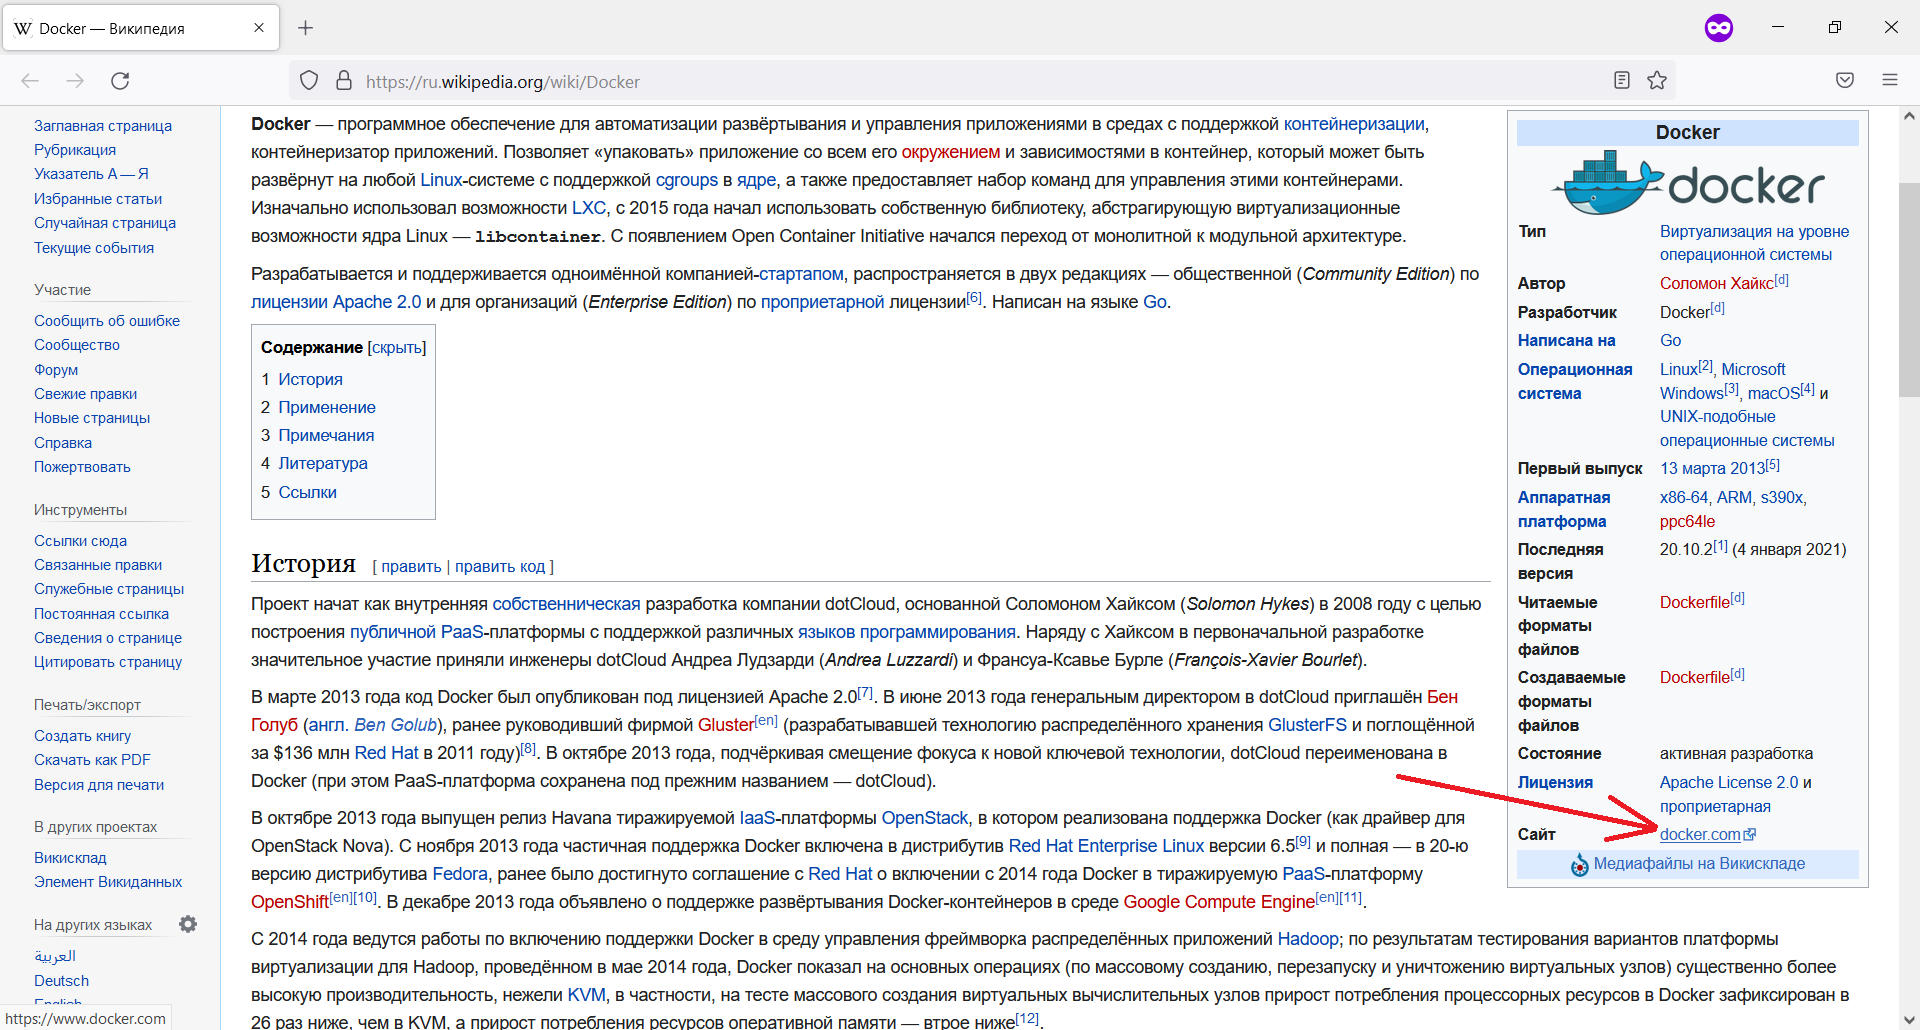
\includegraphics[width=\linewidth]
            {_assets/gpi_pz_docker_01.png}
        \caption{Находим сайт на Wikipedia}
        \label{fig:gpi_pz_docker_01}
    \end{minipage}
    \begin{minipage}{0.47\textwidth}
        \centering
        
\includegraphics[width=\linewidth]
            {_assets/gpi_pz_docker_02.png}
        \caption{Открываем сайт}
        \label{fig:gpi_pz_docker_02}
    \end{minipage}
\end{figure}

\begin{figure}[!p]
    \centering
    \begin{minipage}{0.47\textwidth}
        \centering
        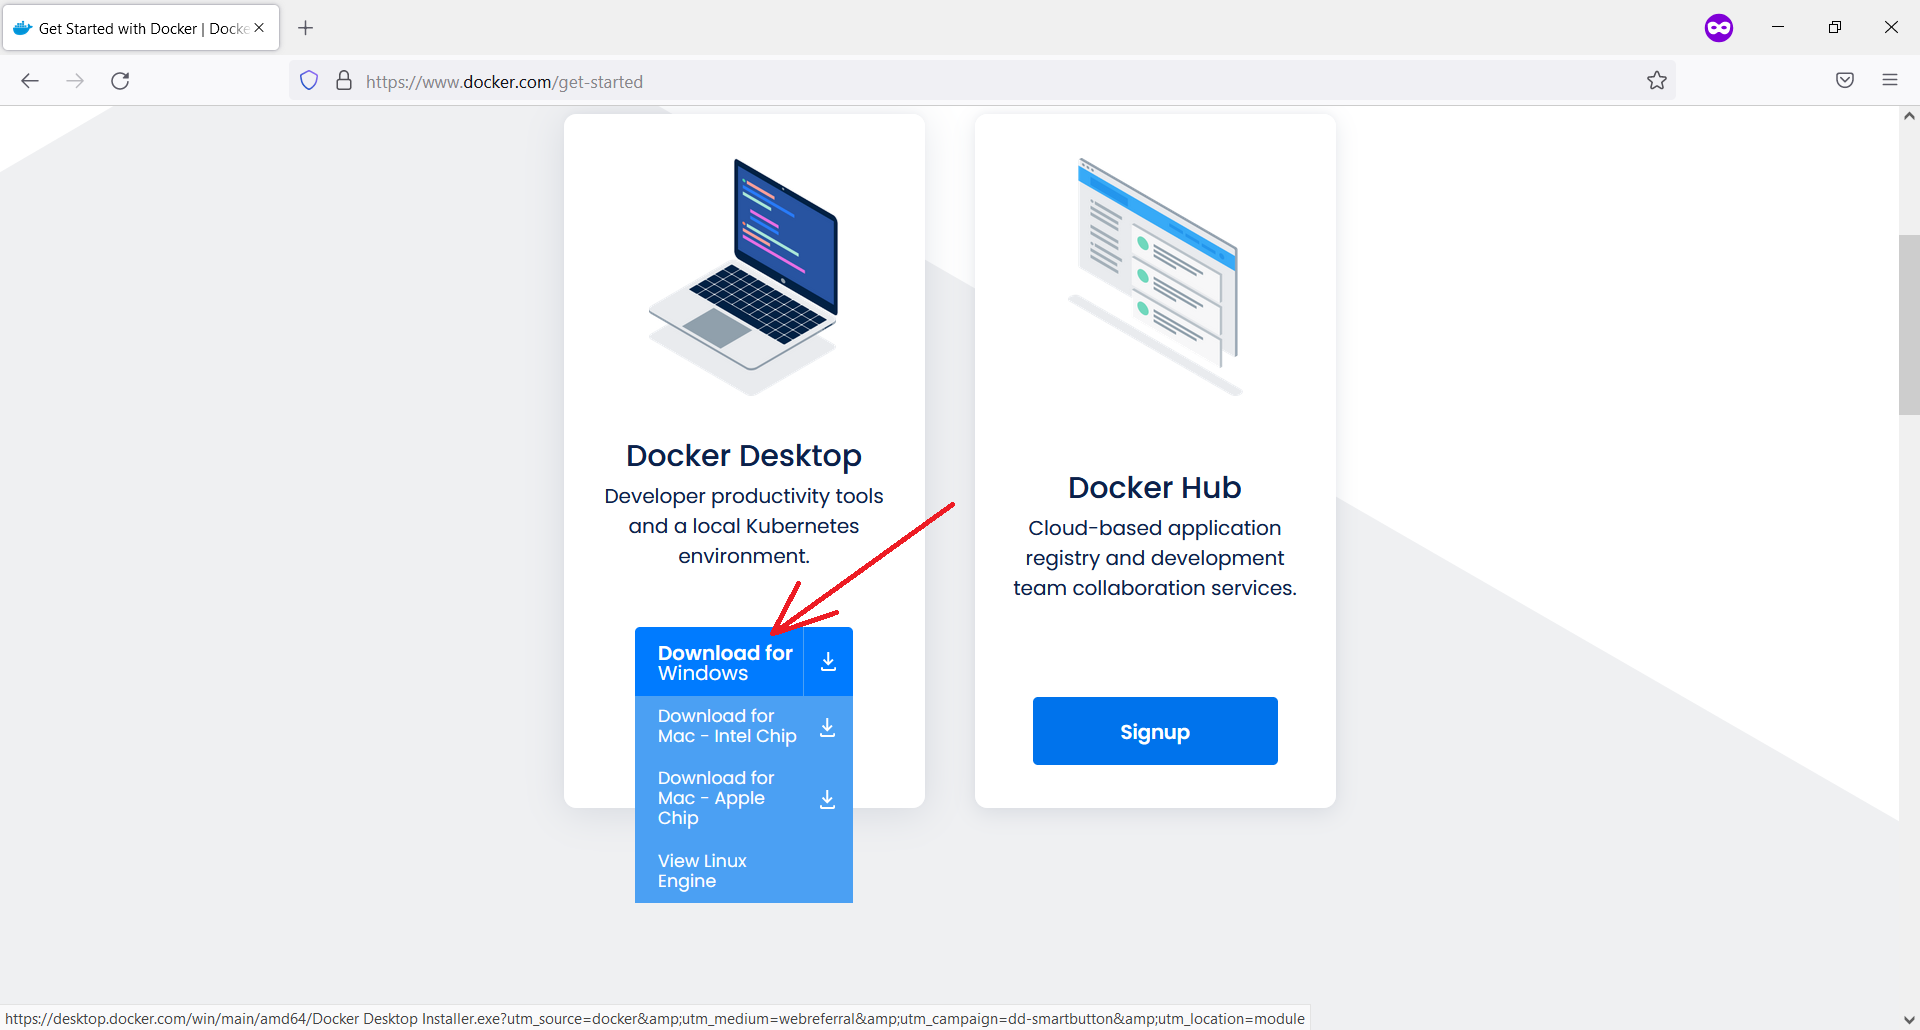
\includegraphics[width=\linewidth]
            {_assets/gpi_pz_docker_03.png}
        \caption{Выбираем установщик Windows}
        \label{fig:gpi_pz_docker_03}
    \end{minipage}
    \begin{minipage}{0.47\textwidth}
        \centering
        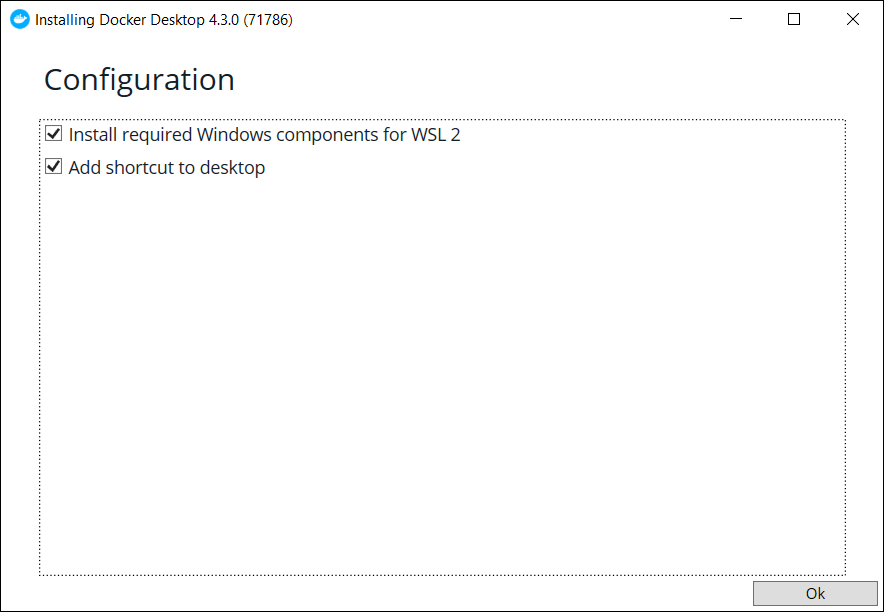
\includegraphics[width=\linewidth]
            {_assets/gpi_pz_docker_04.png}
        \caption{Запускаем файл и устанавливаем Docker}
        \label{fig:gpi_pz_docker_04}
    \end{minipage}
\end{figure}

\begin{figure}[!p]
    \centering
    \begin{minipage}{0.47\textwidth}
        \centering
        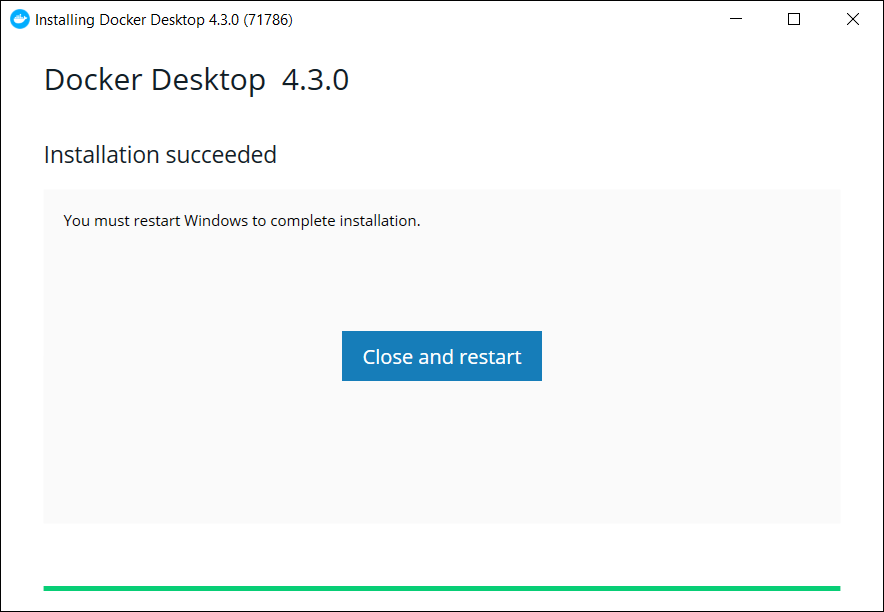
\includegraphics[width=\linewidth]
            {_assets/gpi_pz_docker_05.png}
        \caption{Перезагружаем компьютер}
        \label{fig:gpi_pz_docker_05}
    \end{minipage}
    \begin{minipage}{0.47\textwidth}
        \centering
        
\includegraphics[width=\linewidth]
            {_assets/gpi_pz_docker_06.png}
        \caption{Принимаем лицензию}
        \label{fig:gpi_pz_docker_06}
    \end{minipage}
\end{figure}

\begin{figure}[!p]
    \centering
    \begin{minipage}{0.47\textwidth}
        \centering
        
\includegraphics[width=\linewidth]
            {_assets/gpi_pz_docker_07.png}
        \caption{Ошибка (нет WSL2). Переходим на сайт}
        \label{fig:gpi_pz_docker_07}
    \end{minipage}
    \begin{minipage}{0.47\textwidth}
        \centering
        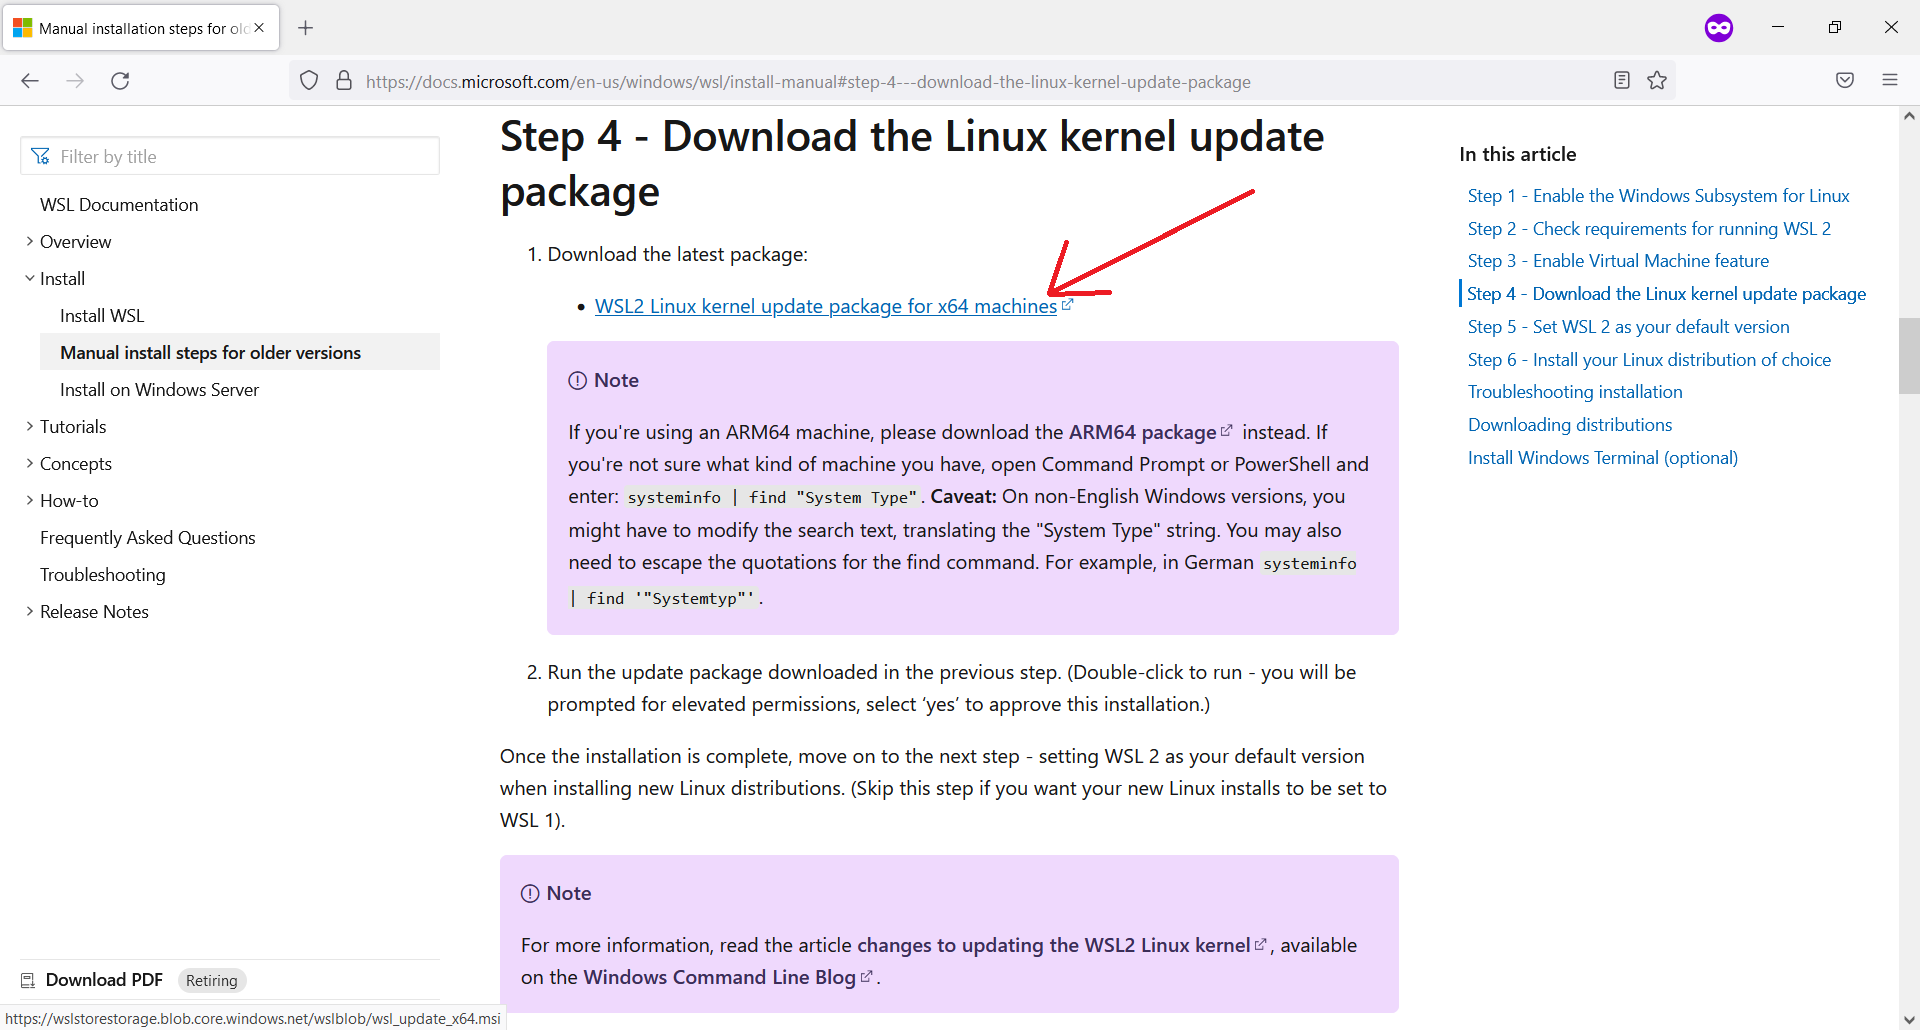
\includegraphics[width=\linewidth]
            {_assets/gpi_pz_docker_08.png}
        \caption{Качаем WSL2 с сайта}
        \label{fig:gpi_pz_docker_08}
    \end{minipage}
\end{figure}

\begin{figure}[!p]
    \centering
    \begin{minipage}{0.47\textwidth}
        \centering
        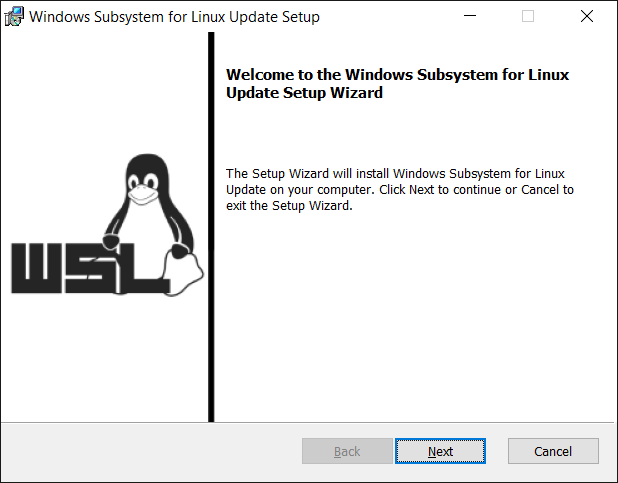
\includegraphics[width=\linewidth]
            {_assets/gpi_pz_docker_09.png}
        \caption{Устанавливаем обновление WSL2}
        \label{fig:gpi_pz_docker_09}
    \end{minipage}
    \begin{minipage}{0.47\textwidth}
        \centering
        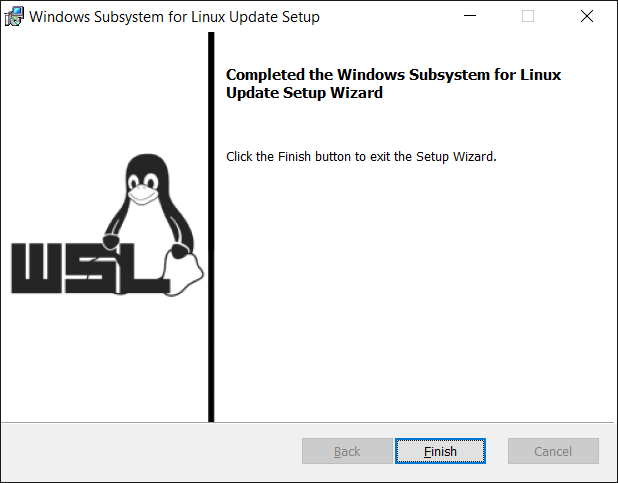
\includegraphics[width=\linewidth]
            {_assets/gpi_pz_docker_10.png}
        \caption{Устанавливаем обновление WSL2}
        \label{fig:gpi_pz_docker_10}
    \end{minipage}
\end{figure}

\begin{figure}[!p]
    \centering
    \begin{minipage}{0.47\textwidth}
        \centering
        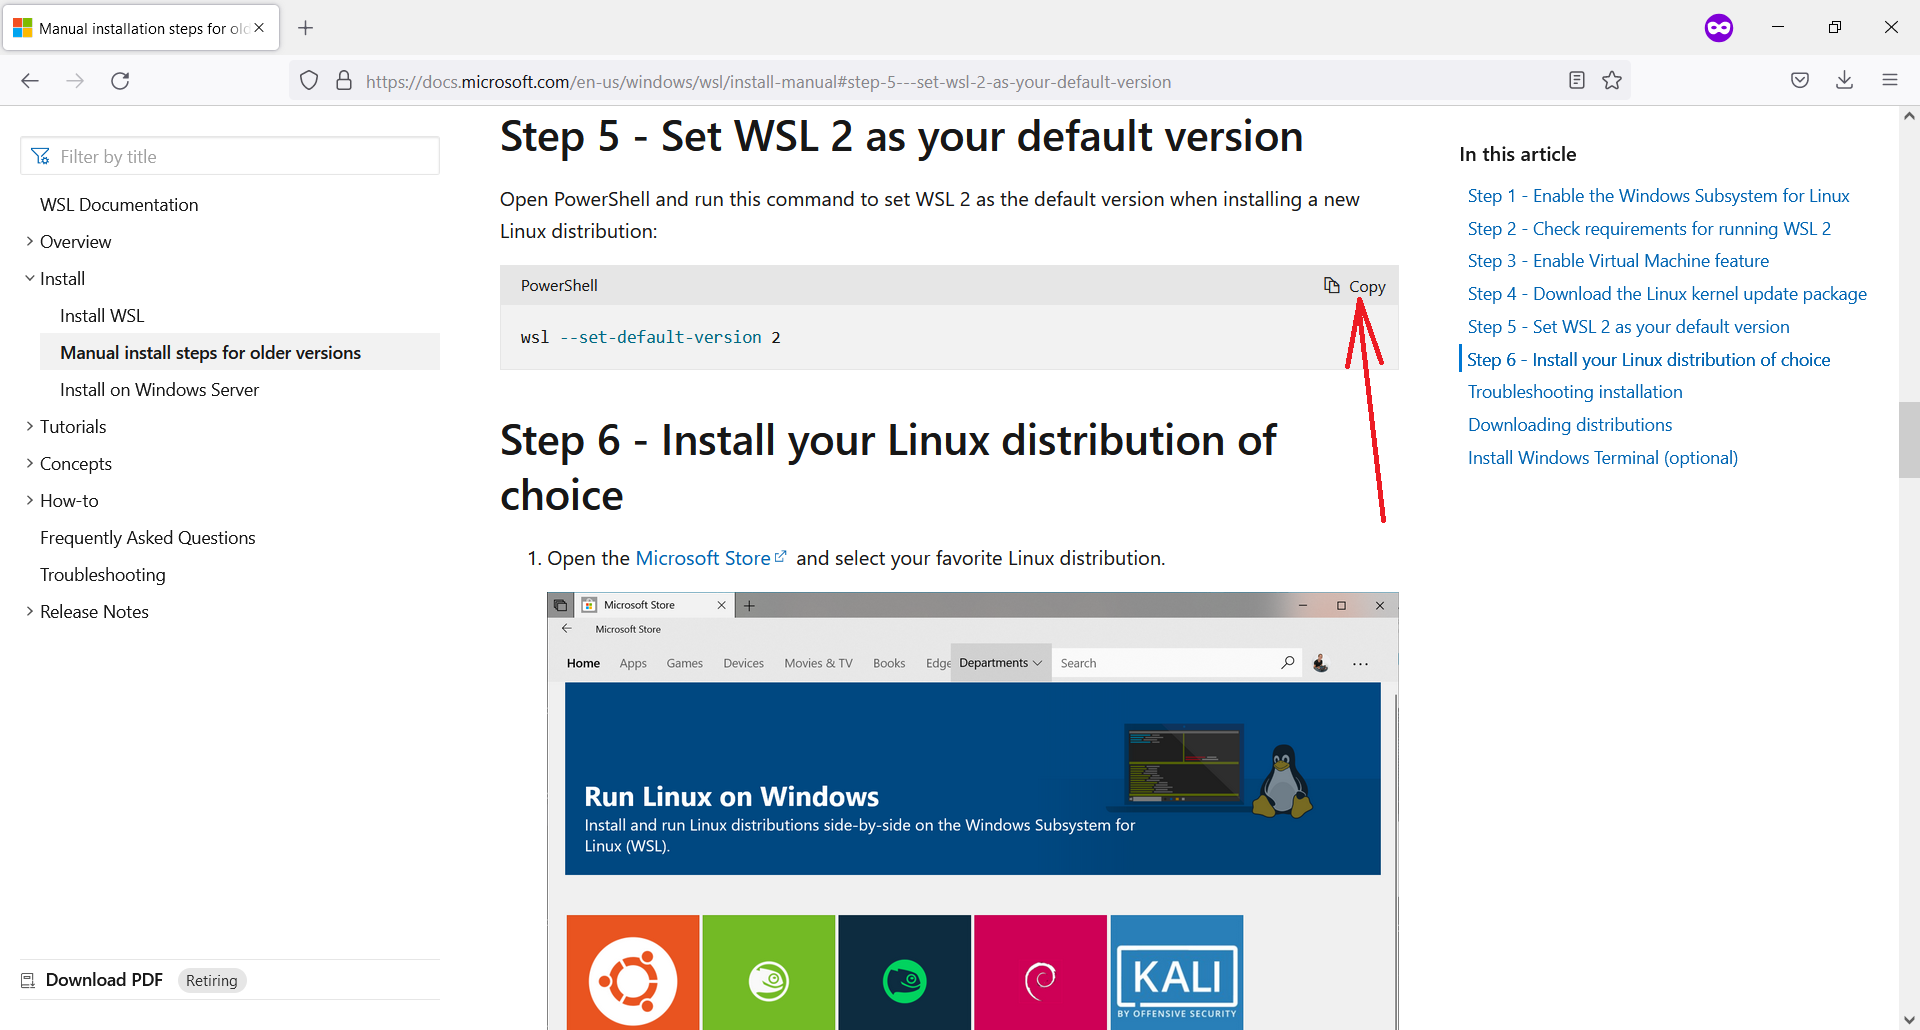
\includegraphics[width=\linewidth]
            {_assets/gpi_pz_docker_11.png}
        \caption{Копируем команду Power Shell, которая поменяет WSL1 на WSL2}
        \label{fig:gpi_pz_docker_11}
    \end{minipage}
    \begin{minipage}{0.47\textwidth}
        \centering
        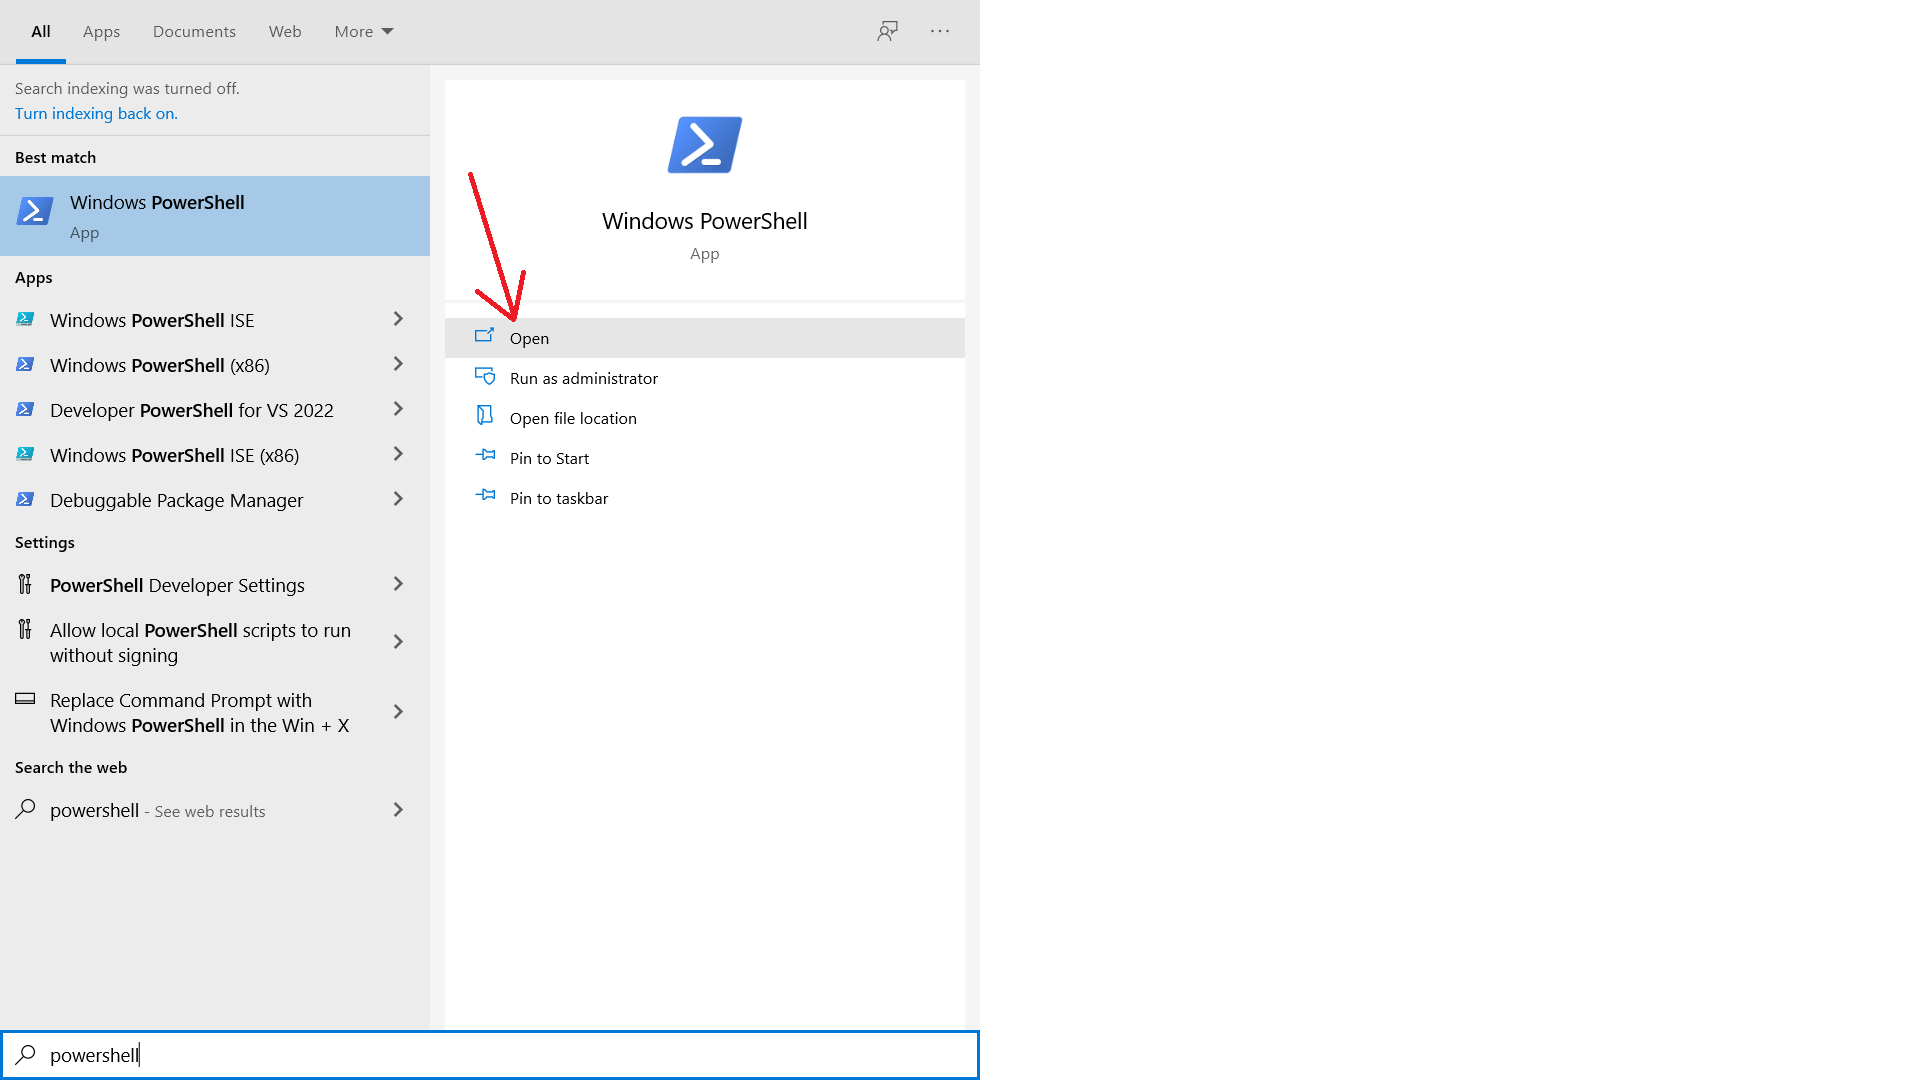
\includegraphics[width=\linewidth]
            {_assets/gpi_pz_docker_12.png}
        \caption{Запускаем поиск, нажав <<Win>> + <<Q>>. Вводим <<powershell>>}
        \label{fig:gpi_pz_docker_12}
    \end{minipage}
\end{figure}

\begin{figure}[!p]
    \centering
    \begin{minipage}{0.47\textwidth}
        \centering
        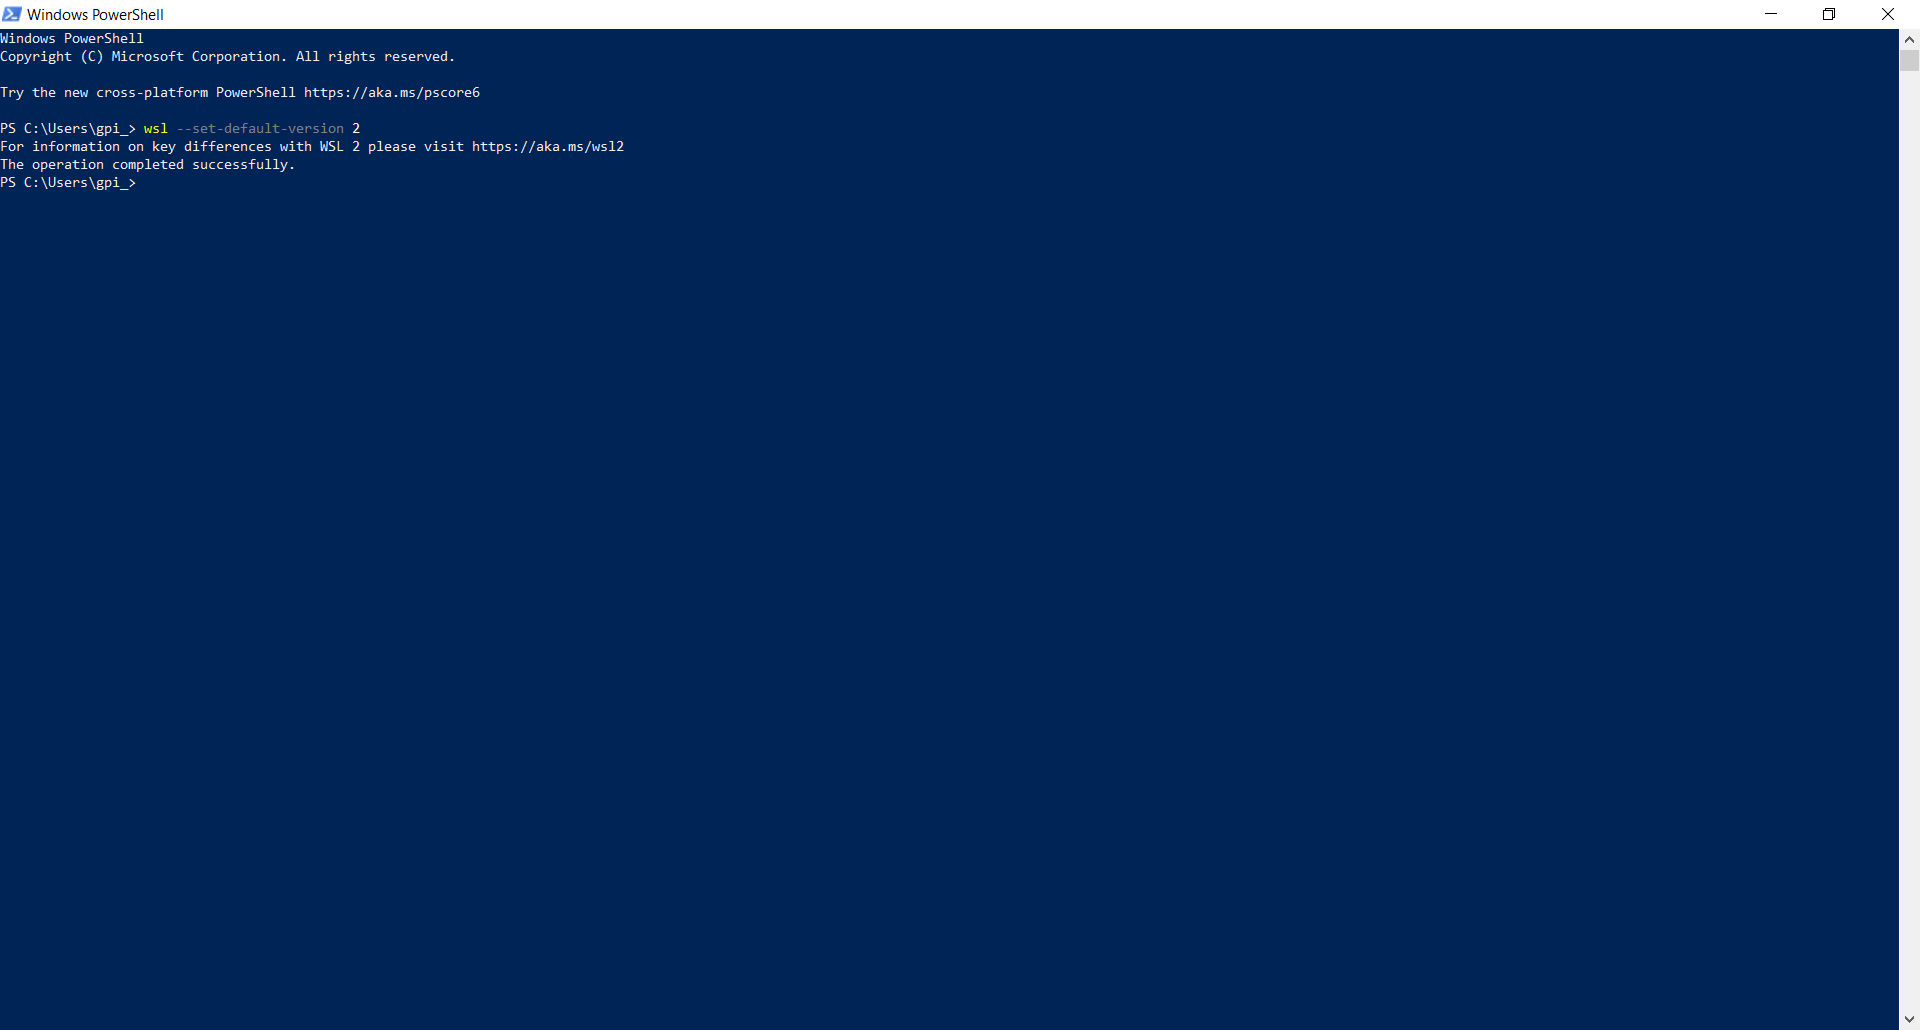
\includegraphics[width=\linewidth]
            {_assets/gpi_pz_docker_13.png}
        \caption{В Power Shell вставляем скопированную команду. \\ Нажимаем <<Enter>> для выполнения}
        \label{fig:gpi_pz_docker_13}
    \end{minipage}
    \begin{minipage}{0.47\textwidth}
        \centering
        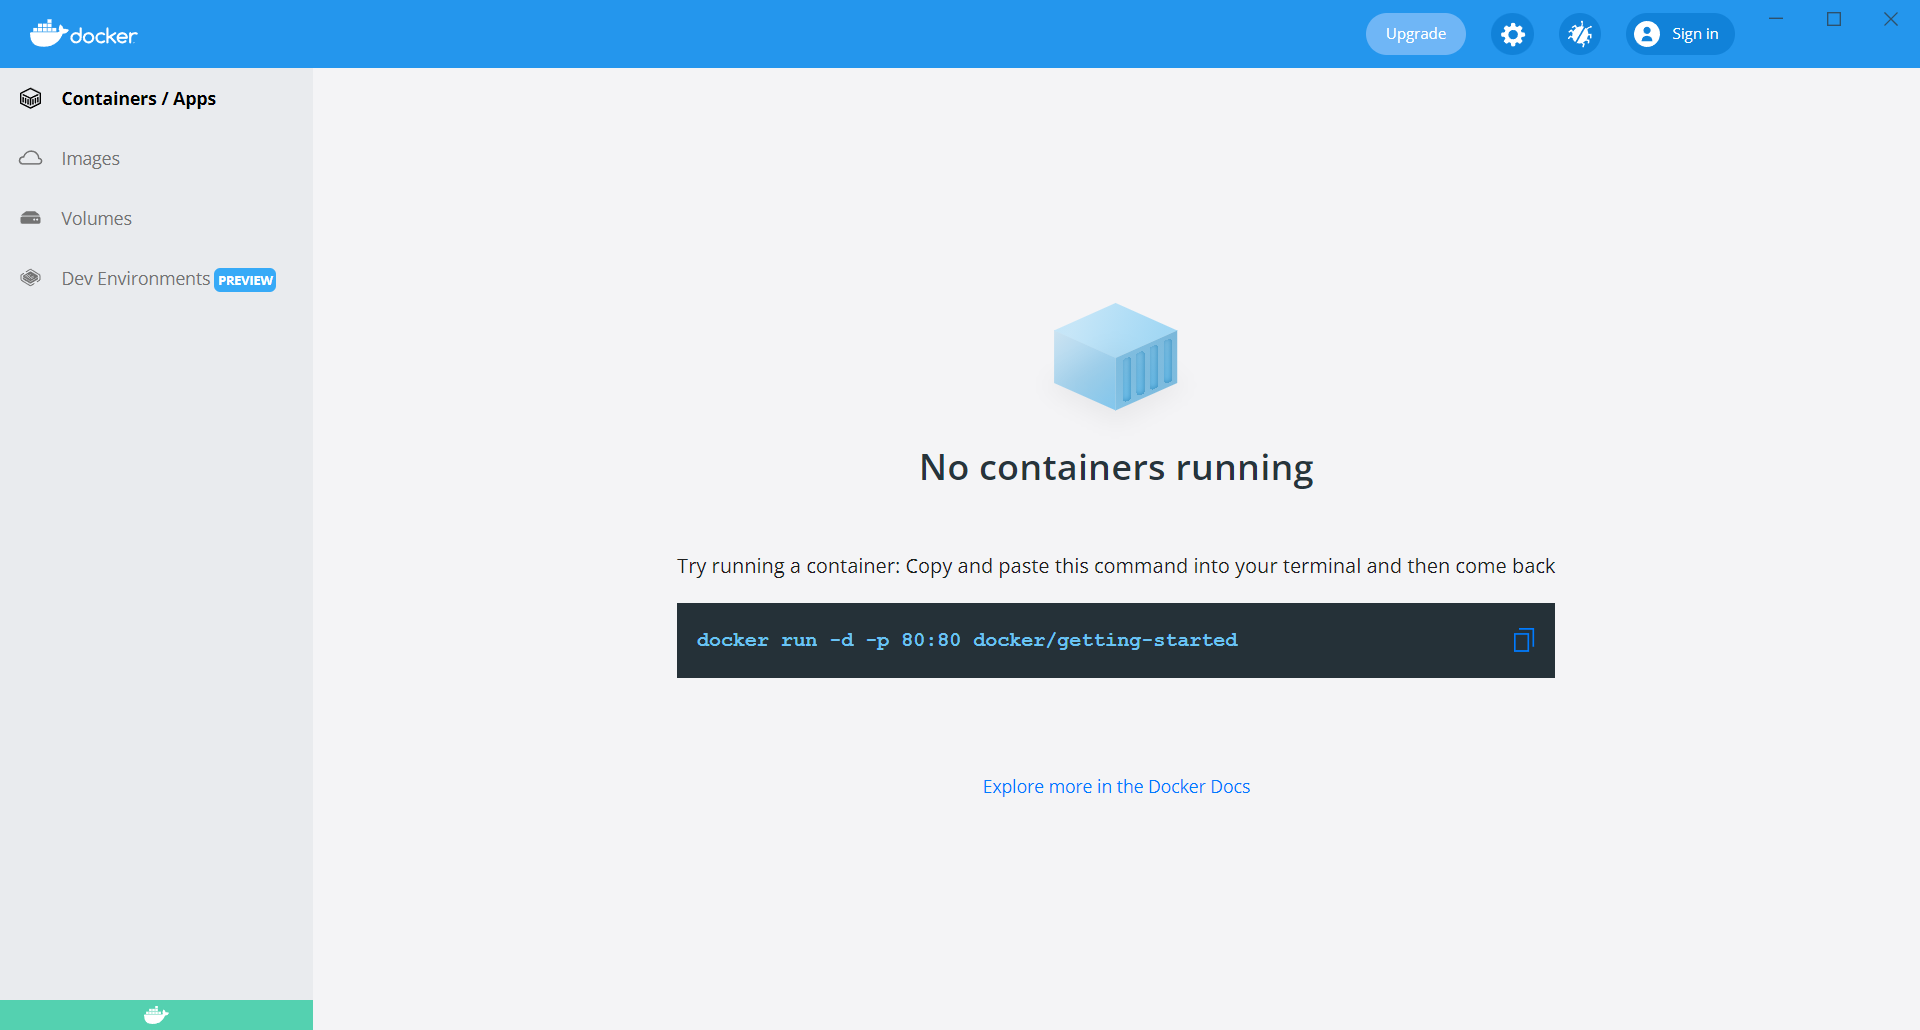
\includegraphics[width=\linewidth]
            {_assets/gpi_pz_docker_14.png}
        \caption{<<Docker Desktop>> запускается без ошибки \\ (но у нас пока нет дистрибутива)}
        \label{fig:gpi_pz_docker_14}
    \end{minipage}
\end{figure}

\begin{figure}[!p]
    \centering
    \begin{minipage}{0.47\textwidth}
        \centering
        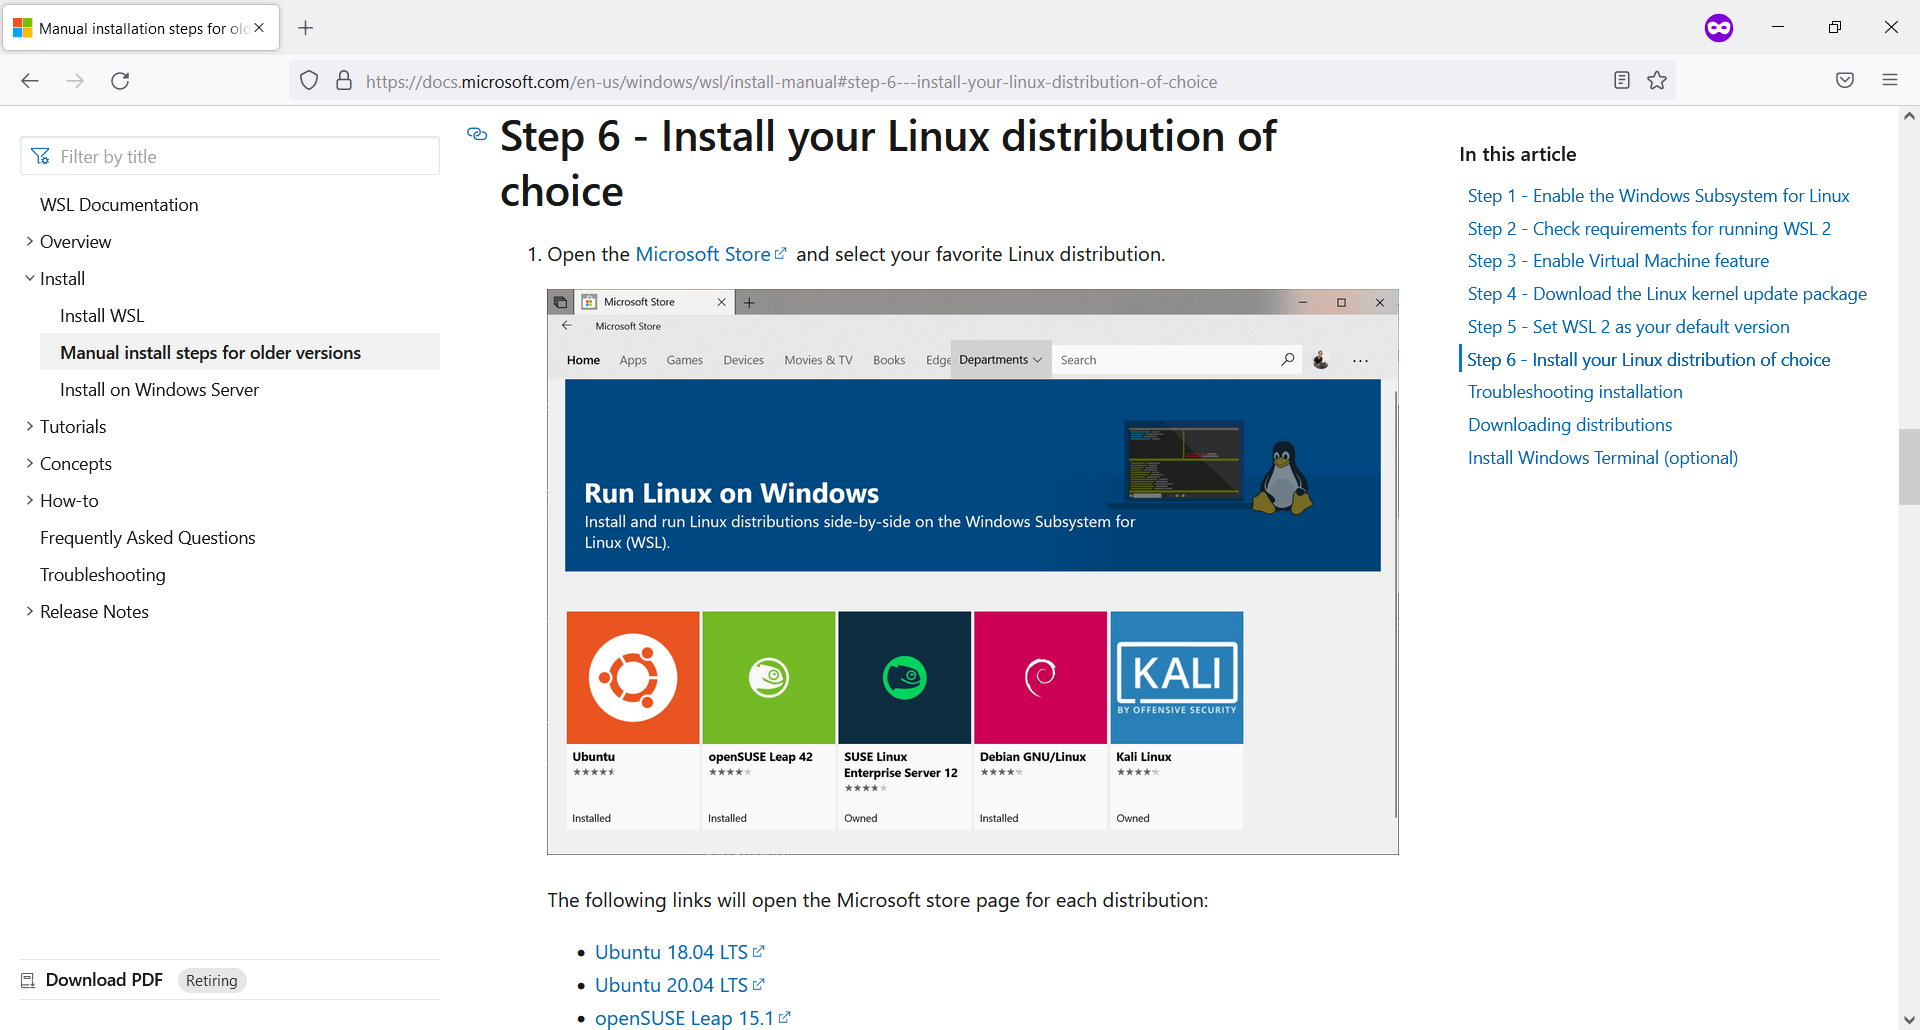
\includegraphics[width=\linewidth]
            {_assets/gpi_pz_docker_15.png}
        \caption{Инструкция говорит скачать дистрибутив Linux}
        \label{fig:gpi_pz_docker_15}
    \end{minipage}
    \begin{minipage}{0.47\textwidth}
        \centering
        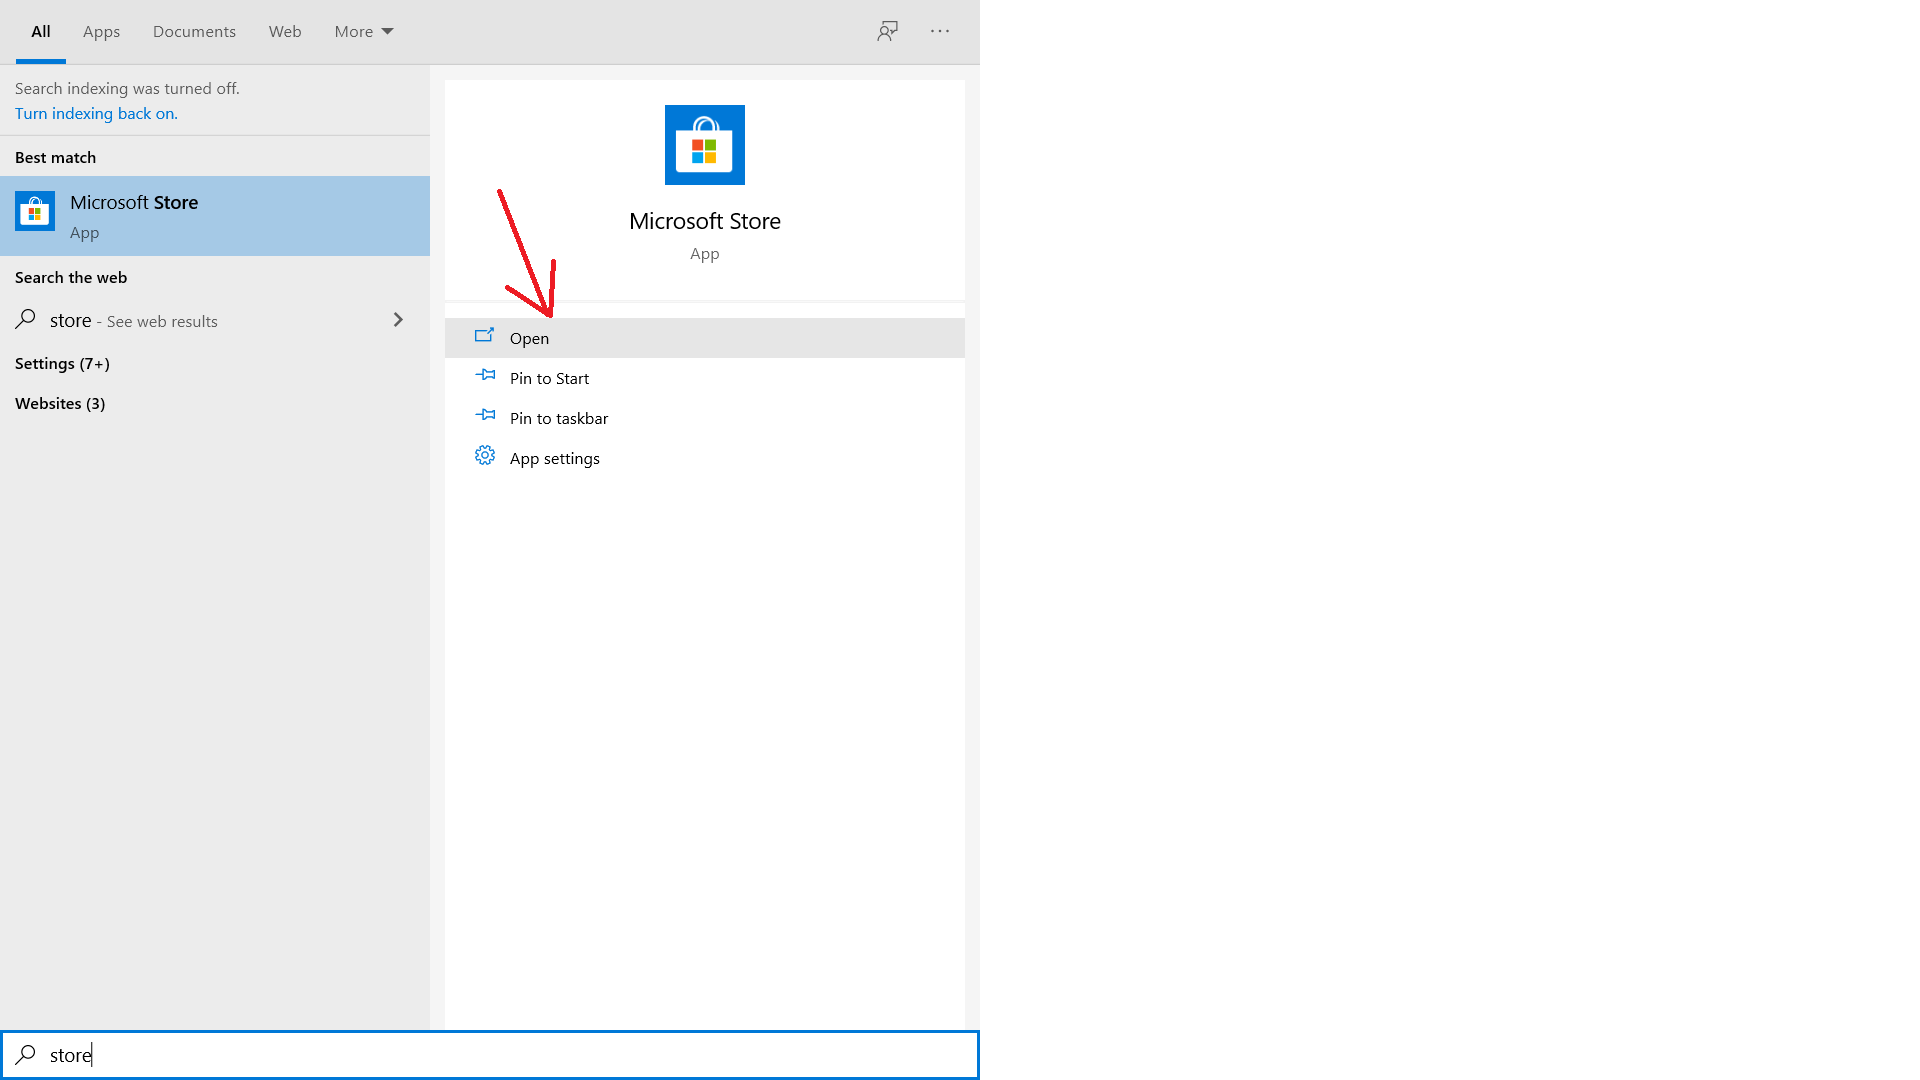
\includegraphics[width=\linewidth]
            {_assets/gpi_pz_docker_16.png}
        \caption{Запускаем поиск, нажав Win + Q, - и вводим <<Store>>}
        \label{fig:gpi_pz_docker_16}
    \end{minipage}
\end{figure}

\begin{figure}[!p]
    \centering
    \begin{minipage}{0.47\textwidth}
        \centering
        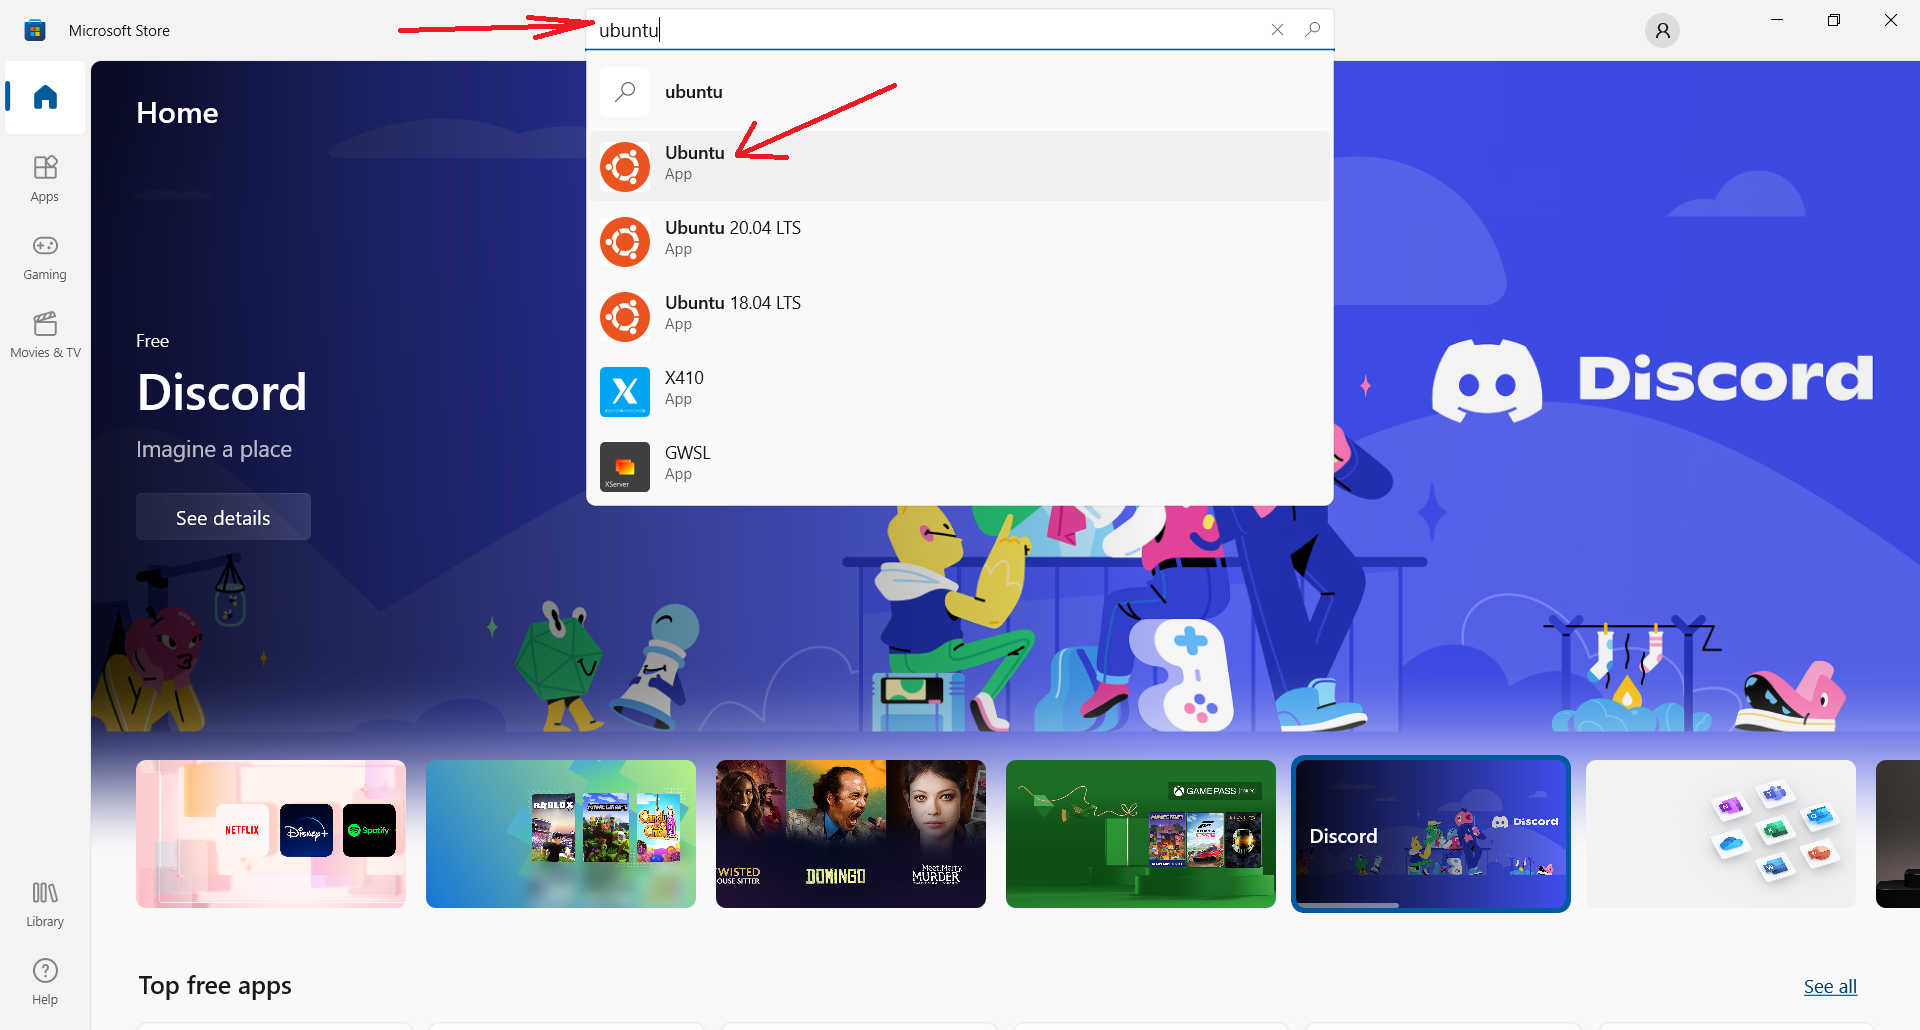
\includegraphics[width=\linewidth]
            {_assets/gpi_pz_docker_17.png}
        \caption{Открываем поиск, вводим <<Ubuntu>> и выбираем подходящий вариант}
        \label{fig:gpi_pz_docker_17}
    \end{minipage}
    \begin{minipage}{0.47\textwidth}
        \centering
        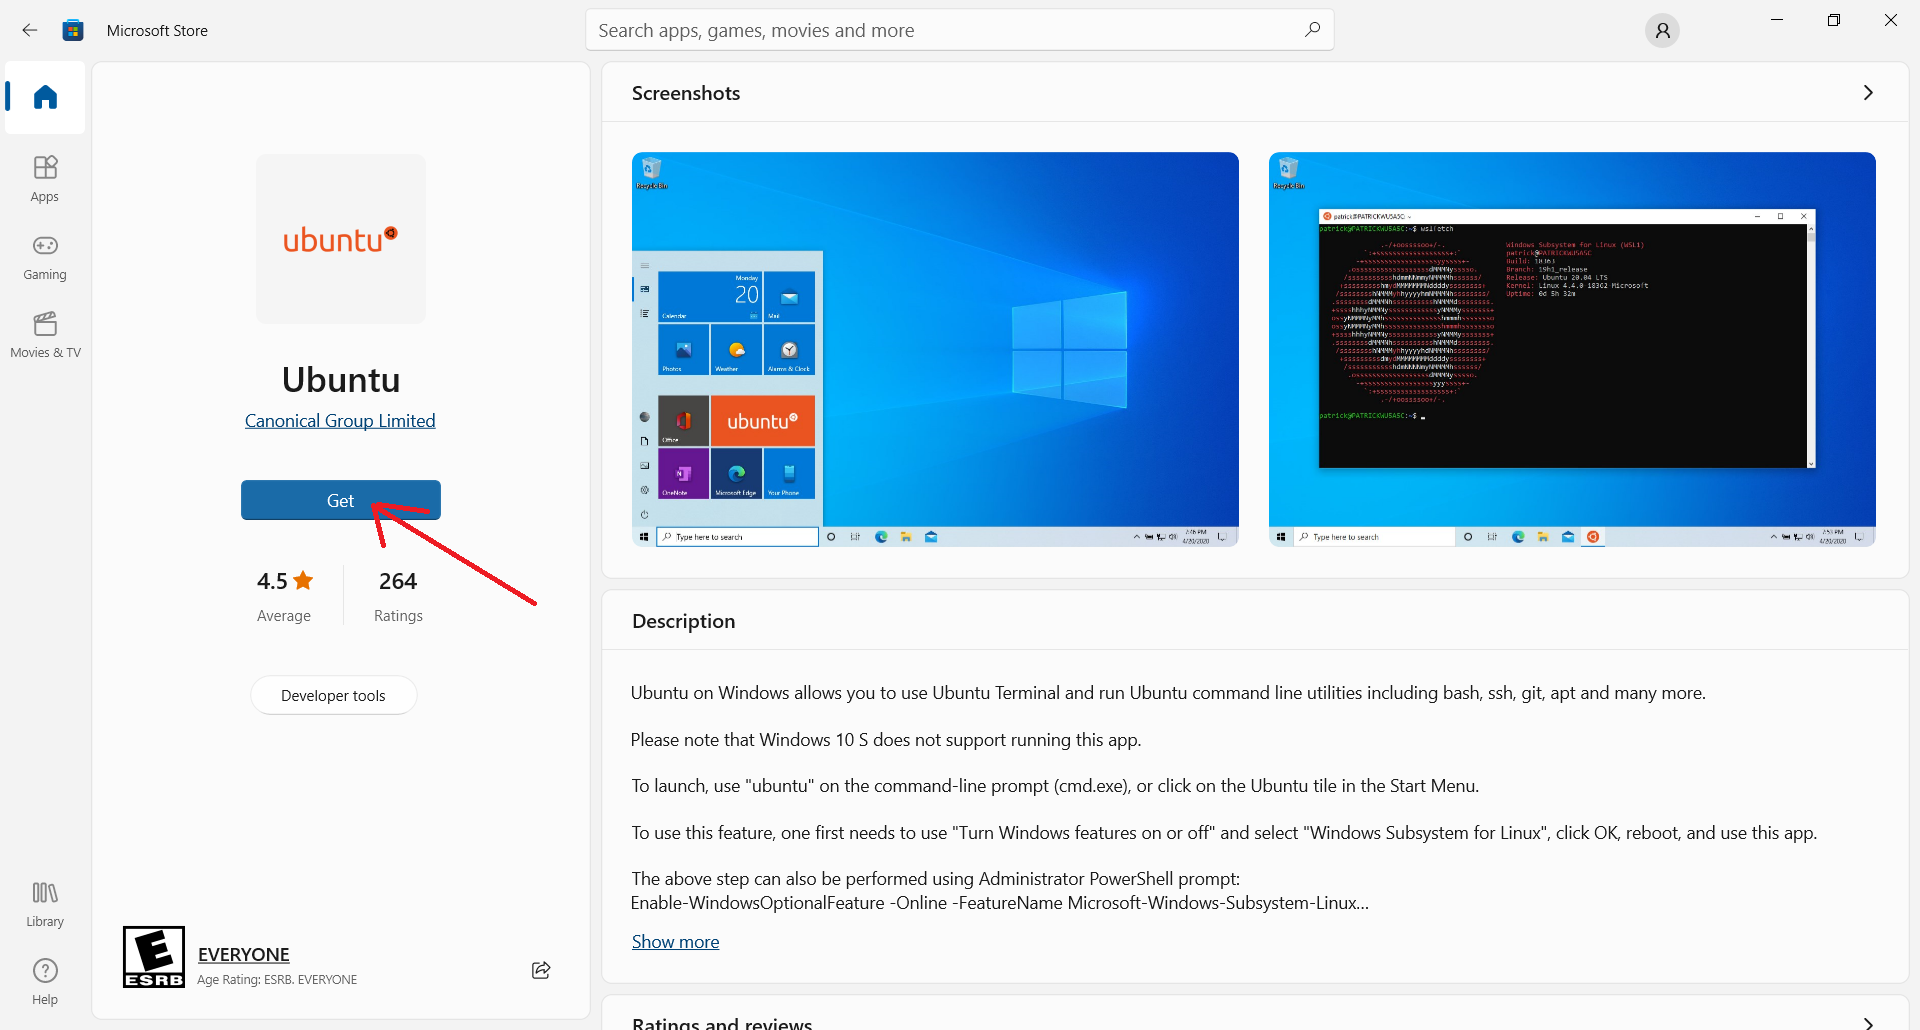
\includegraphics[width=\linewidth]
            {_assets/gpi_pz_docker_18.png}
        \caption{Устанавливаем приложение, нажав на кнопку <<Get>>}
        \label{fig:gpi_pz_docker_18}
    \end{minipage}
\end{figure}

\begin{figure}[!p]
    \centering
    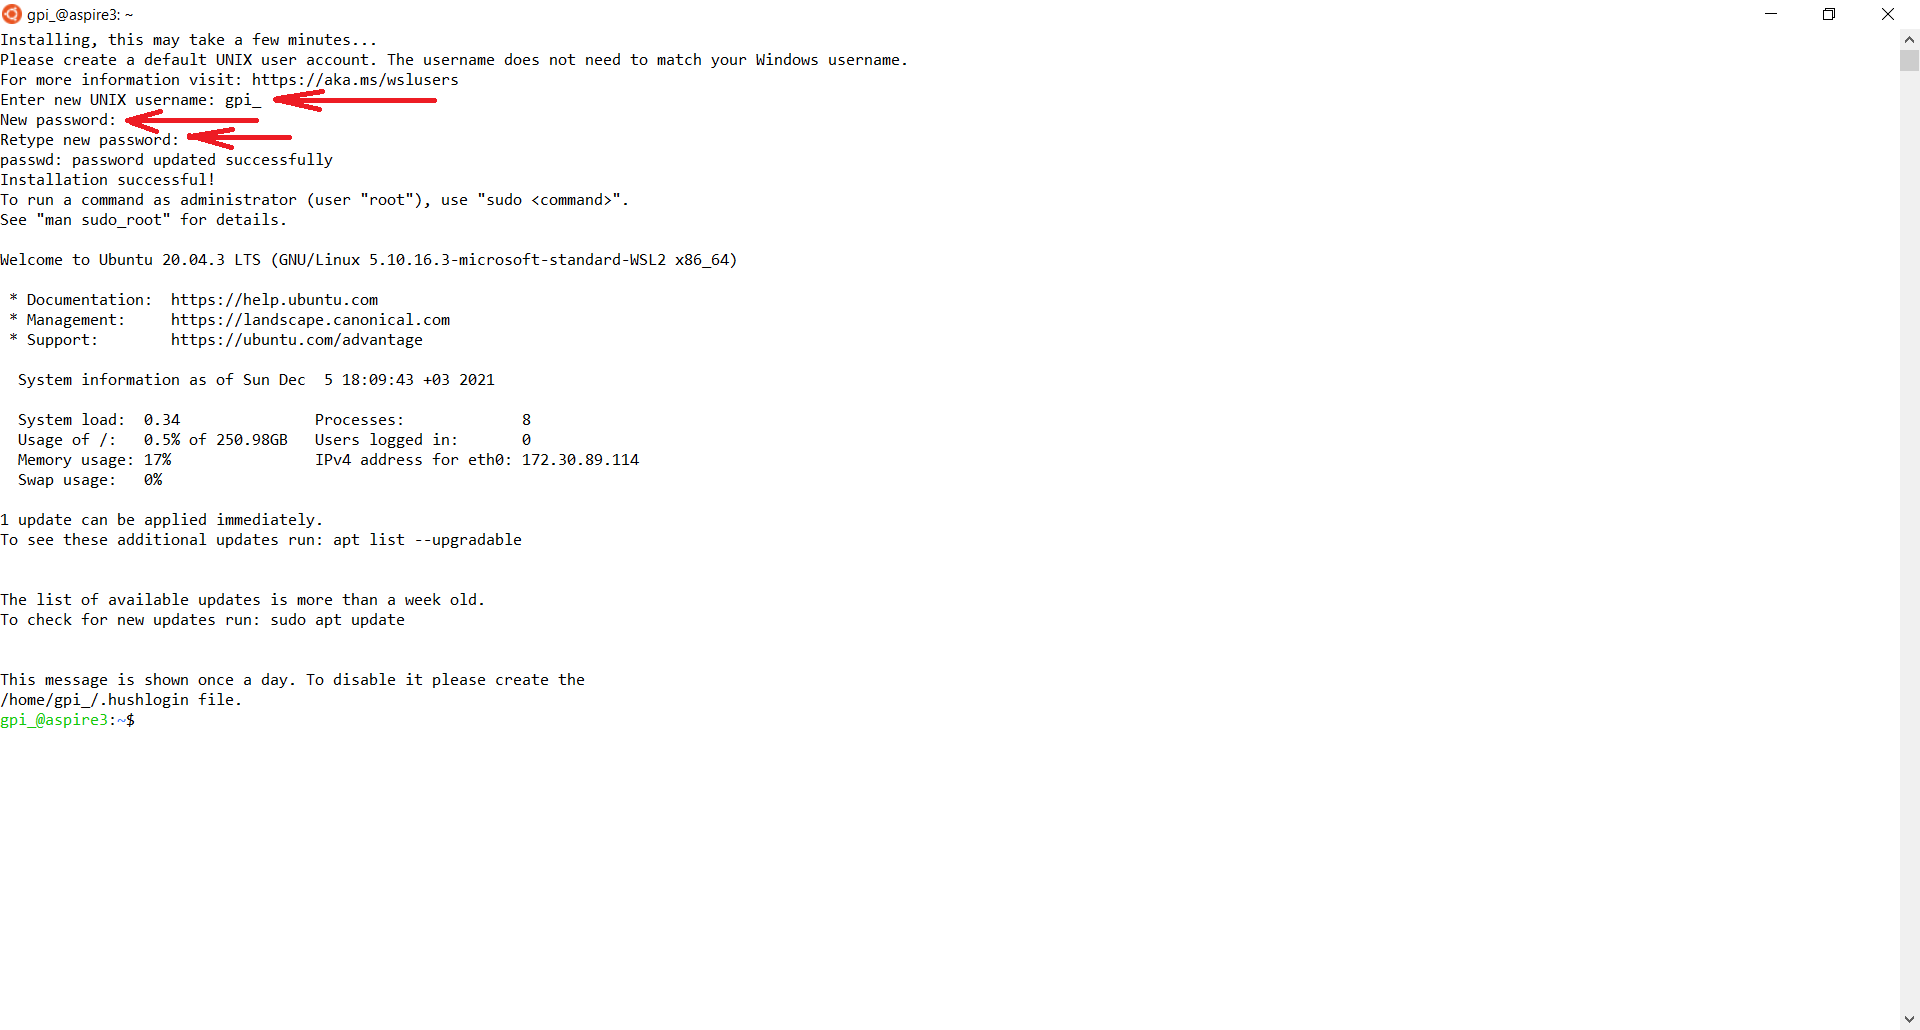
\includegraphics[width=12cm]
        {_assets/gpi_pz_docker_19.png}
    \caption{При первом запуске устанавливаем имя пользователя и пароль для дистрибутива}
    \label{fig:gpi_pz_docker_19}
\end{figure}

\begin{figure}[!p]
    \centering
    \begin{minipage}{0.47\textwidth}
        \centering
        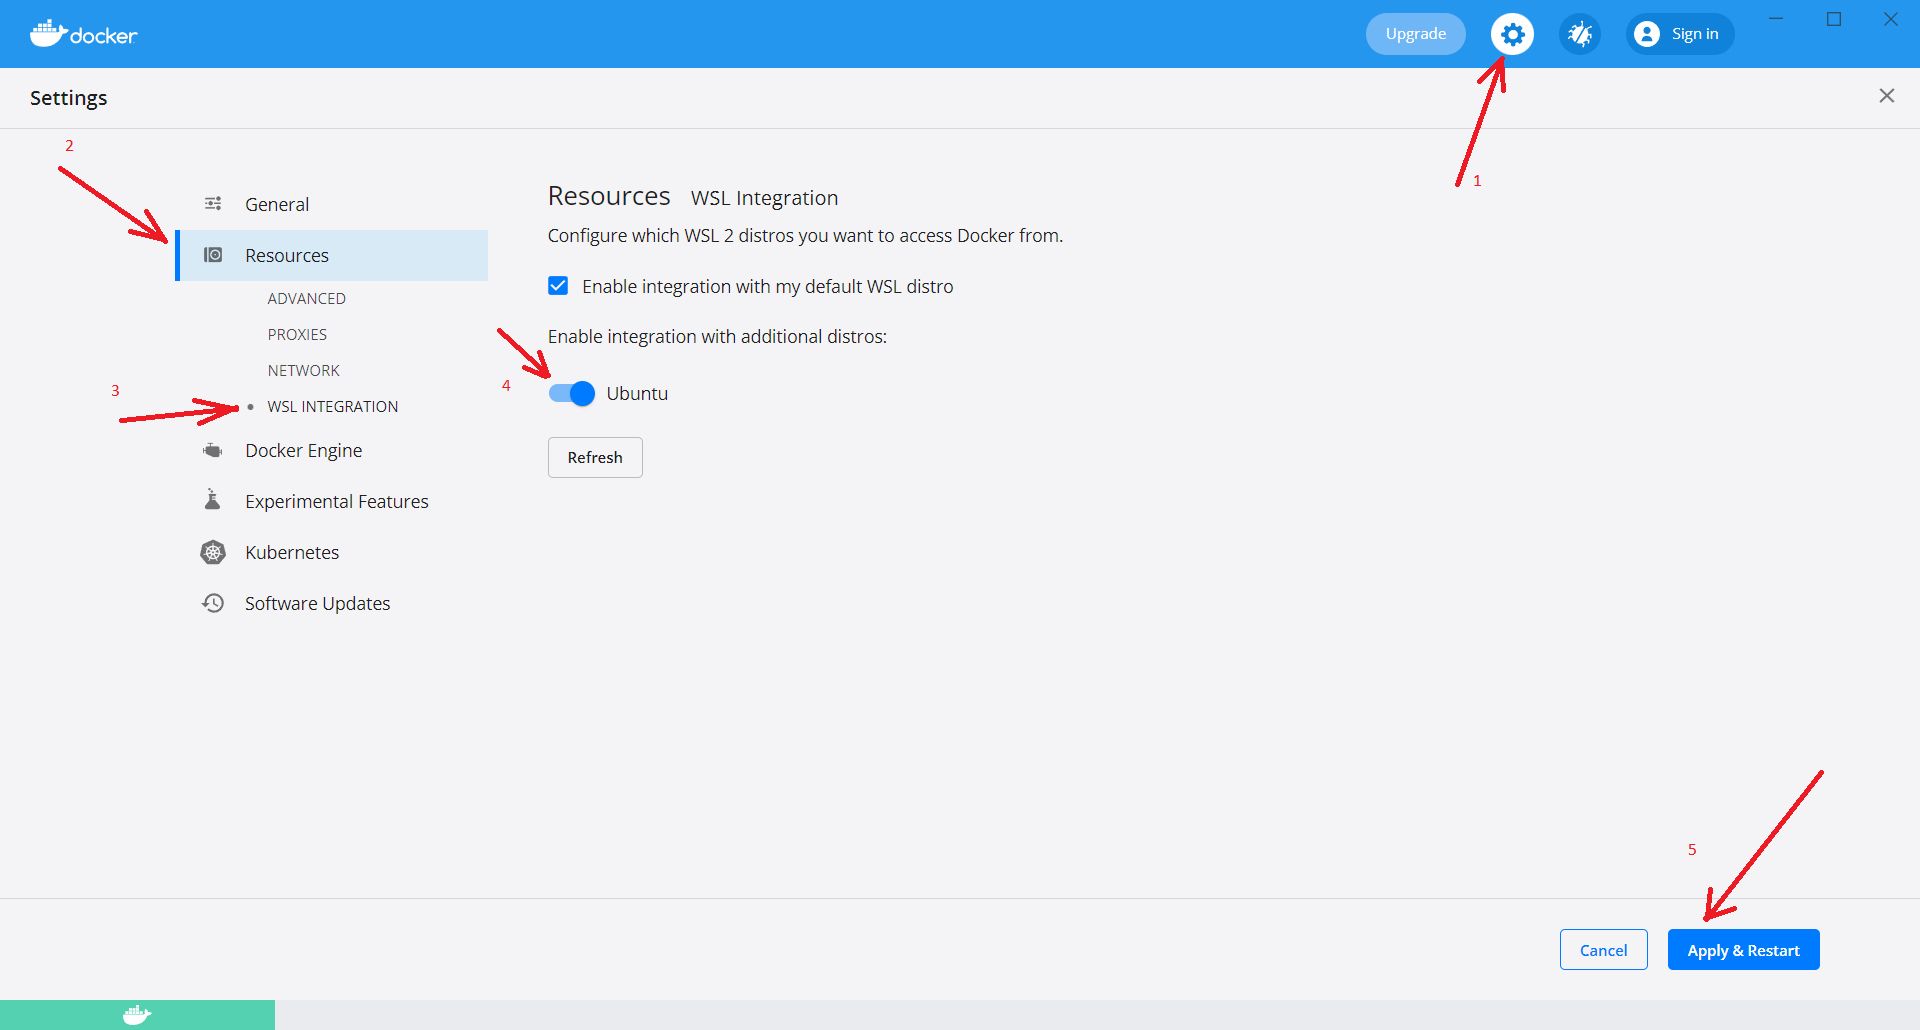
\includegraphics[width=\linewidth]
            {_assets/gpi_pz_docker_20.png}
        \caption{Включаем в приложении работу в дистрибутиве <<Ubuntu>>}
        \label{fig:gpi_pz_docker_20}
    \end{minipage}
    \begin{minipage}{0.47\textwidth}
        \centering
        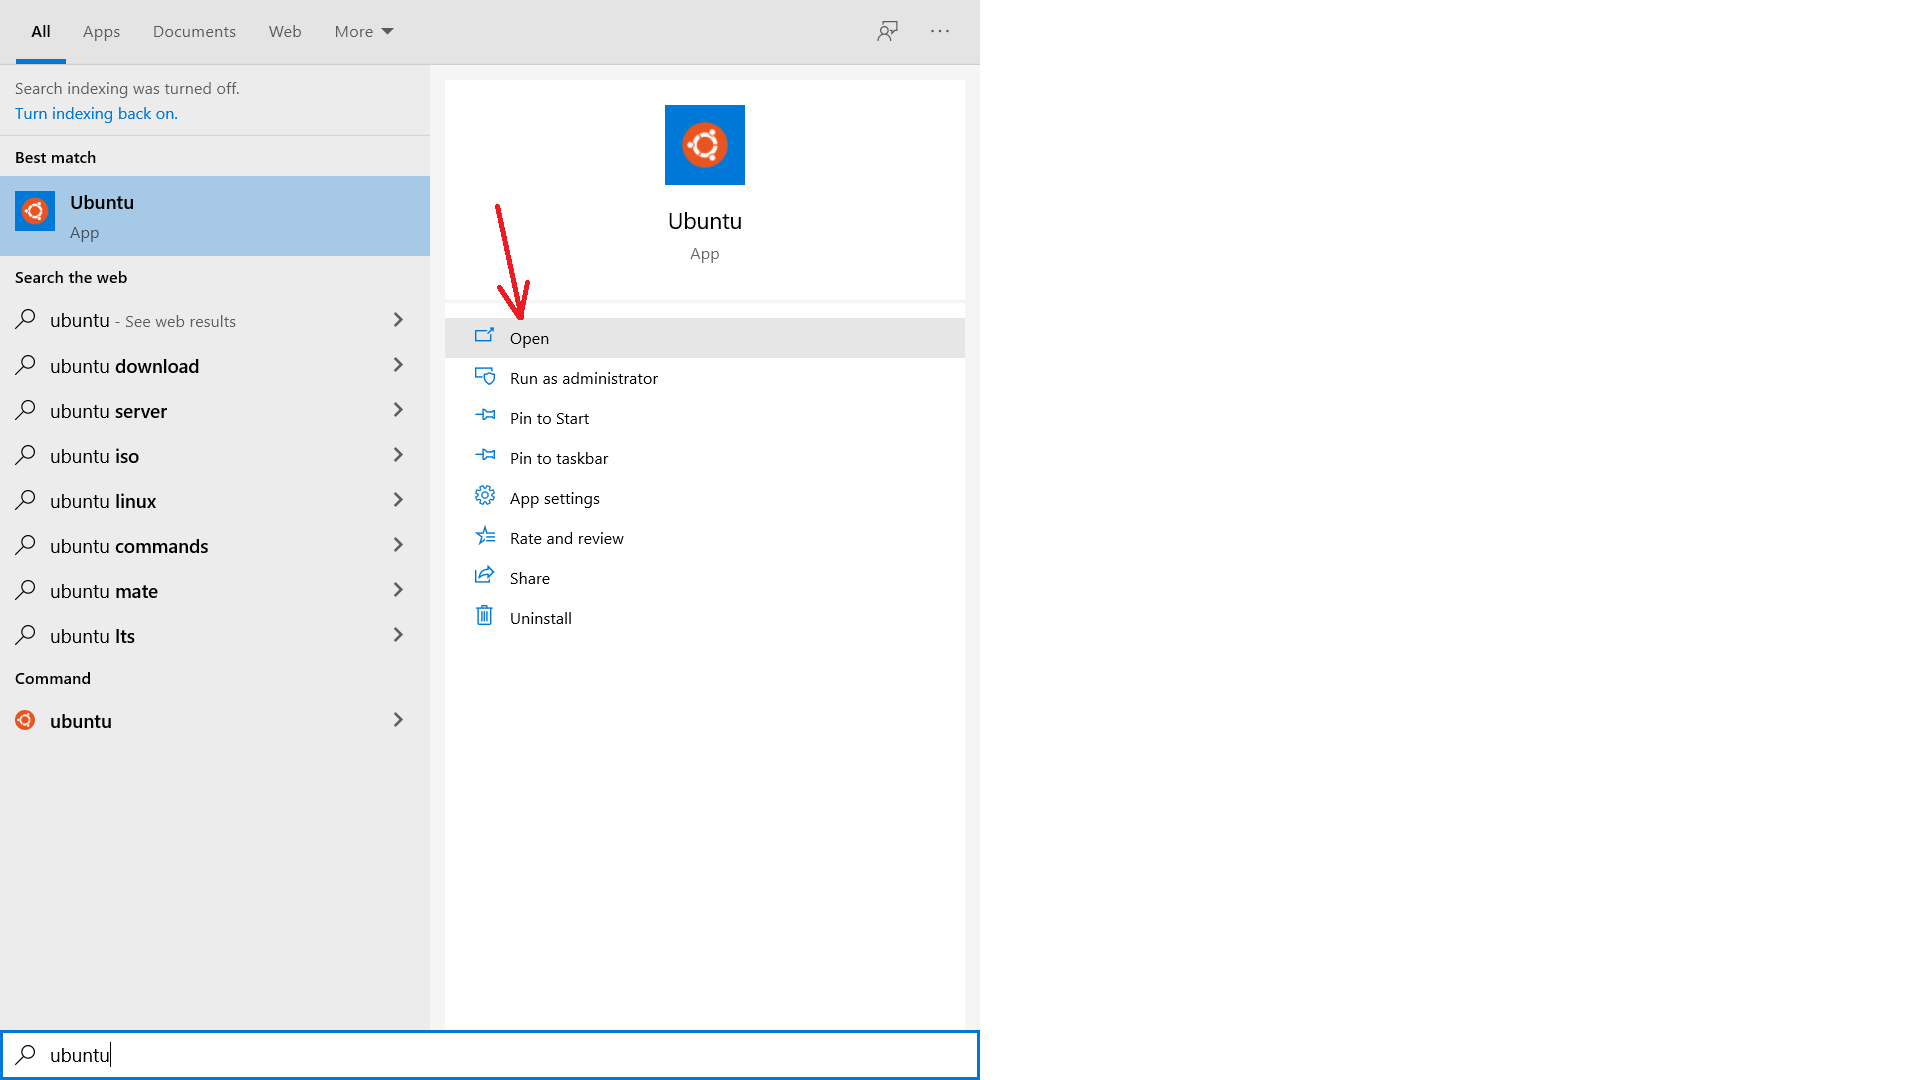
\includegraphics[width=\linewidth]
            {_assets/gpi_pz_docker_21.png}
        \caption{Зажимаем <<Win>> + <<Q>> и в поиске вводим <<Ubuntu>>}
        \label{fig:gpi_pz_docker_21}
    \end{minipage}
\end{figure}

\begin{figure}[!p]
    \centering
    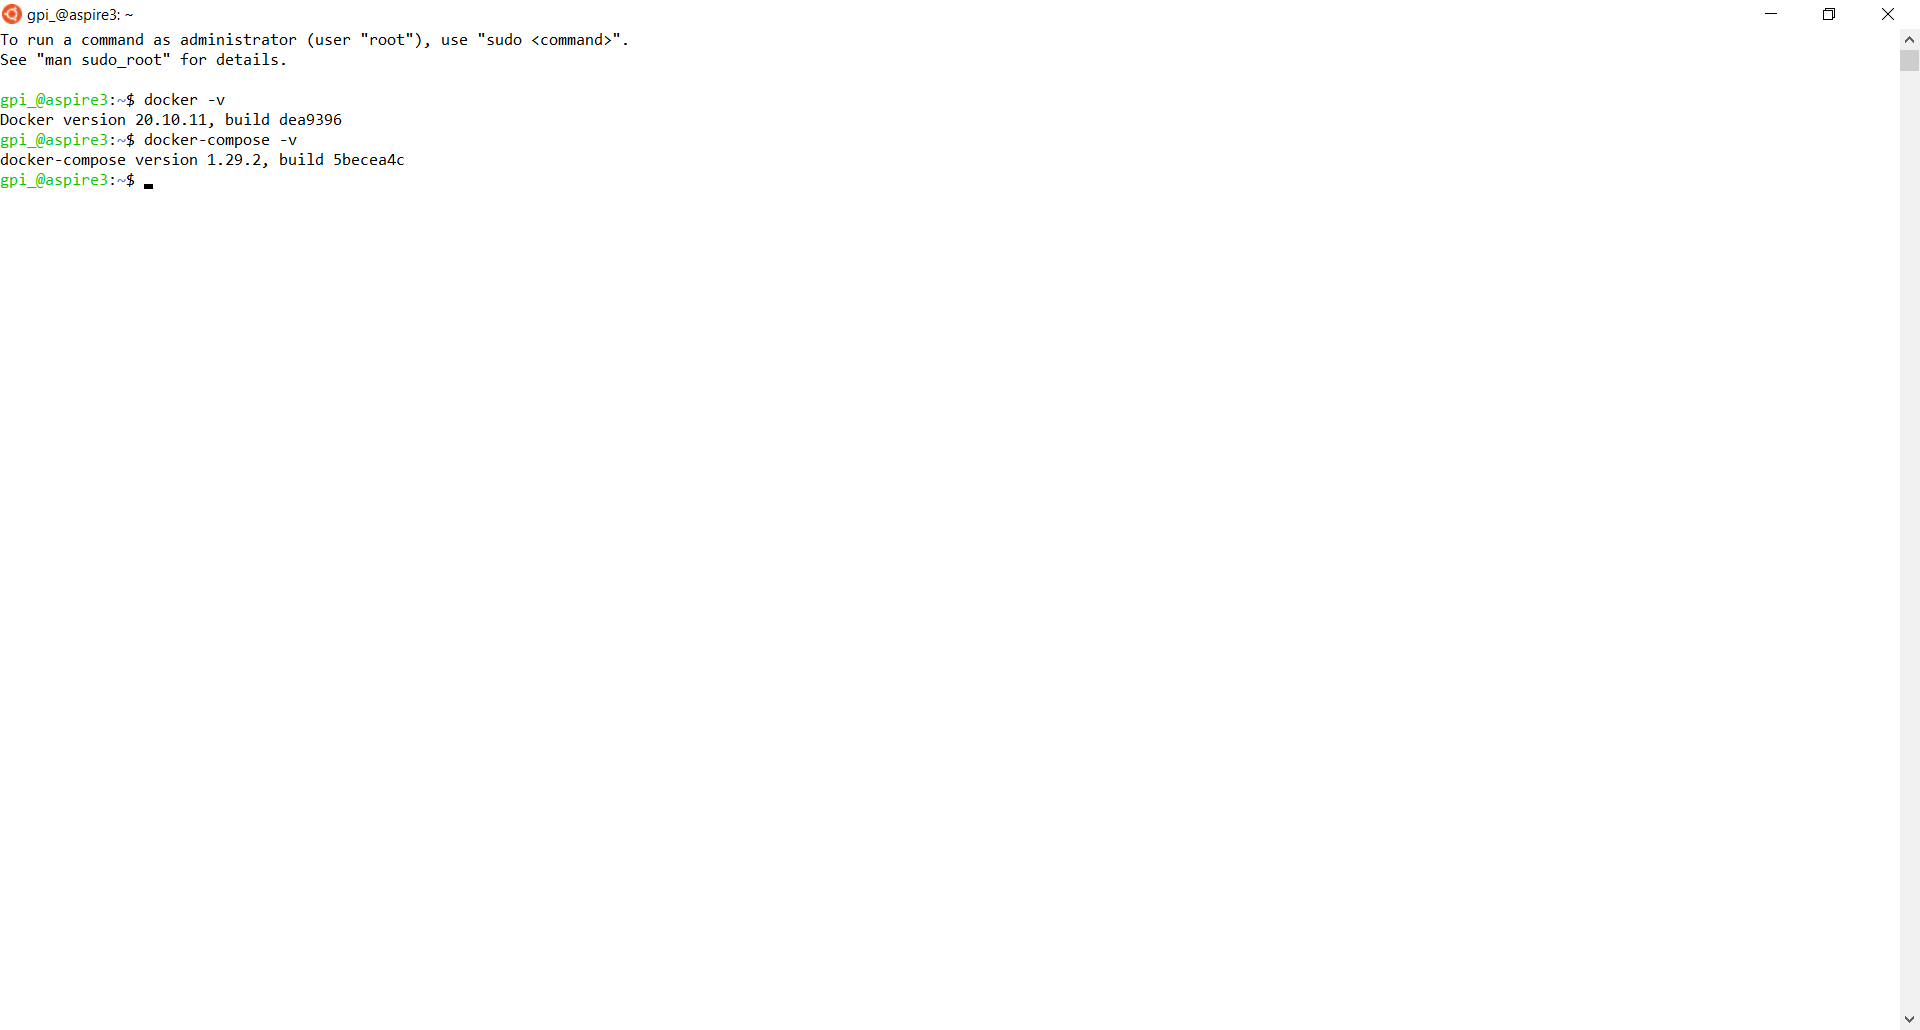
\includegraphics[width=12cm]
        {_assets/gpi_pz_docker_22.png}
    \caption{Убеждаемся в установке Docker, проверив версию Docker и docker-compose}
    \label{fig:gpi_pz_docker_22}
\end{figure}

\newpage

% = = = = = = = = = = = = = = = =

\subsection{Скрипты для запуска (Makefile)}

В ходе написания курсовой работы были разработаны следующие проекты:

\begin{itemize}
    \item Backend для API на Express.
    \item Frontend для панели администратора на React.
    \item Frontend для интернет-магазина на React.
    \item LAMP для MySQL.
\end{itemize}

Для того чтобы запускать каждый проект нужено входить в каждую папку (папку проекта)
и запускать свой скрипт. Было принято решение записать все команды в один файл - Makefile,
который находится в корне репозитория.

\lstinputlisting[
    name=\textbf{Листинг: Makefile},
    language=make,
    numbers=none,
]
    {../Makefile}

\newpage
         % 3. Реализация системы
    \newpage

\section{Тестирование системы}

% Тестирование веб-приложений – это комплекс услуг,
% который может включать в себя различные виды тестирования ПО.

% Основная цель любого тестирования,
% в том числе и тестирования веб-приложений, - обнаружить все ошибки в программном обеспечении
% и разработать рекомендации по их предотвращению в будущем.

% \subsection{Тестирование верстки}
% \subsection{Функциональное тестирование}
% \subsection{Usability тестирование (User Experience)}
% \subsection{Тестирование совместимости (конфигурационное тестирование)}
% \subsection{Тестирование производительности}
% \subsection{Тестирование безопасности}
% \subsection{Регрессионное тестирование}

\subsection{Описание входных и выходных данных}

В базе данных MySQL храняться следующие таблицы

\begin{itemize}
    \item \textbf{admins} - таблица для хранения логинов администратора и их захэшированные пароли.
    Скриншот на \textbf{рис.~\ref{fig:gpi_pz_mysql_admins} (стр.~\pageref{fig:gpi_pz_mysql_admins})}.
    \item \textbf{products} - таблица для зранения данных о продукте.
    Скриншот на \textbf{рис.~\ref{fig:gpi_pz_mysql_products} (стр.~\pageref{fig:gpi_pz_mysql_products})}.
\end{itemize}

\begin{figure}[!h]
    \centering
    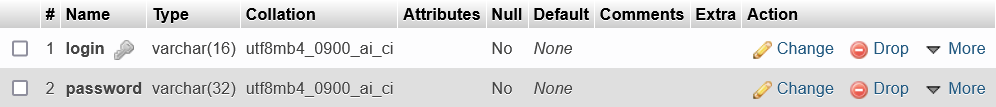
\includegraphics[width=16cm]
        {_assets/gpi_pz_mysql_admins.png}
    \caption{MySQL таблица admins}
    \label{fig:gpi_pz_mysql_admins}
\end{figure}

\begin{figure}[!h]
    \centering
    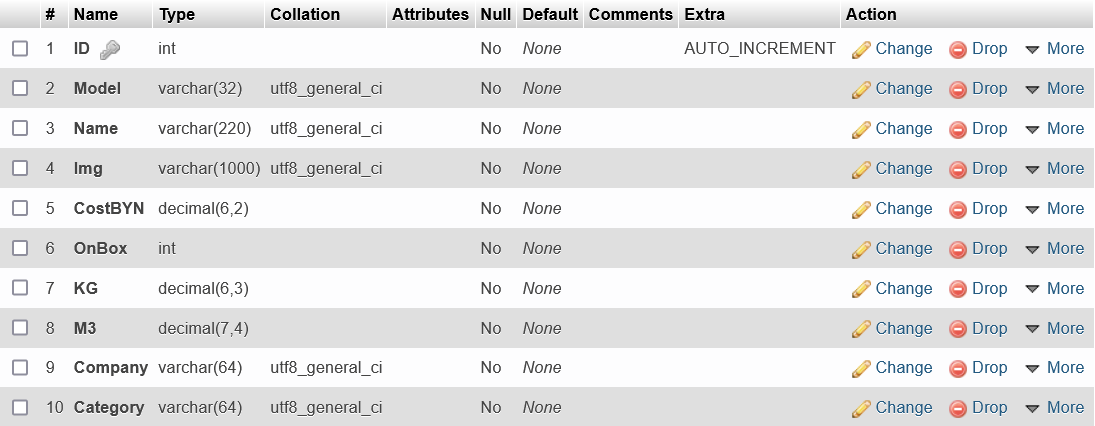
\includegraphics[width=16cm]
        {_assets/gpi_pz_mysql_products.png}
    \caption{MySQL таблица products}
    \label{fig:gpi_pz_mysql_products}
\end{figure}

\newpage

\subsection{Тестирование приложения}

Среда тестирования: 

\begin{itemize}
    \item \textbf{ПК} Acer Aspire 3:
    \begin{itemize}
    \item processor - AMD Ryzen 3 3250U with  Radeon Graphics 2.60 GHz;
    \item installed memory (RAM) - 4.00 (3.44 GB usable);
    \item system type - 64-bit Operating System, x64-based processor.
    \end{itemize}
    \item \textbf{Браузер} Mozilla Firefox 91.4.0esr (64-bit).
    \item \textbf{БД} - MySQL 8.0.27.
    \item \textbf{Виртуальная машина} - Docker 20.10.11, docker-compose 2.2.1.
    \item \textbf{Сборщик проекта} - Make 4.3.
    \item \textbf{Сервер} - Express 4.17.1.
\end{itemize}

% = = = = = = = = = = = = = = = = = = = = = = = = = = = = = = = =

\subparagraph{Тестируемая задача:} <<Авторизация в панели администратора с неверным вводом данных: логина или пароля>>

\textit{Ожидаемый результат}: администратор не авторизуется - сервер отправит результат о не подходящем логине или пароле,
браузер сообщит об ошибке.

\textit{Полученный результат}: администратор не аторизовался, браузер сообщил об ошибке.

\textit{Выводы по тесту}: \\
Скриншот сообщения о несуществовании логина на
\textbf{рис.~\ref{fig:gpi_pz_auth_error_login} (стр.~\pageref{fig:gpi_pz_auth_error_login})}.\\
Скриншот сообщения о неправильном пароле на
\textbf{рис.~\ref{fig:gpi_pz_auth_error_password} (стр.~\pageref{fig:gpi_pz_auth_error_password})}.

\begin{figure}[!h]
    \centering
    \begin{minipage}{0.47\textwidth}
        \centering
        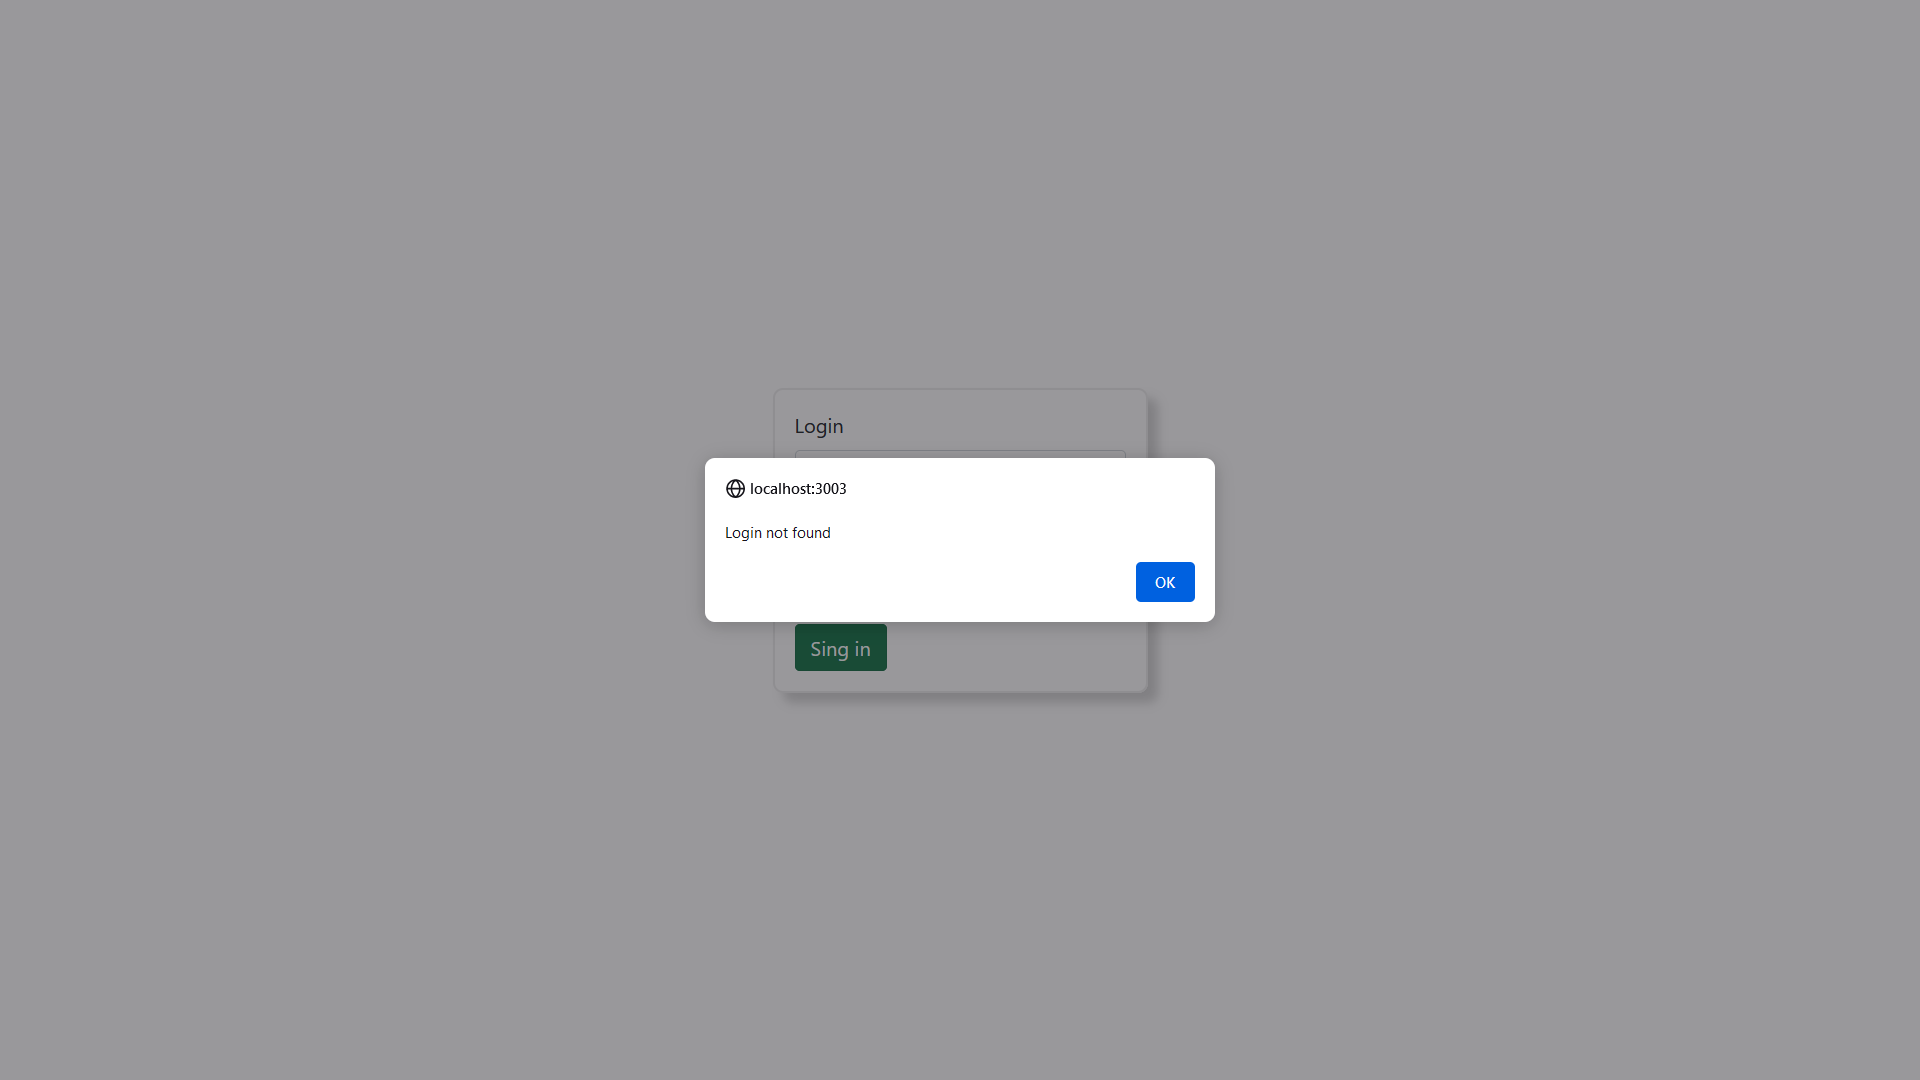
\includegraphics[width=\linewidth]
            {_assets/gpi_pz_auth_error_login.png}
        \caption{Сообщение об несуществовании логина}
        \label{fig:gpi_pz_auth_error_login}
    \end{minipage}
    \begin{minipage}{0.47\textwidth}
        \centering
        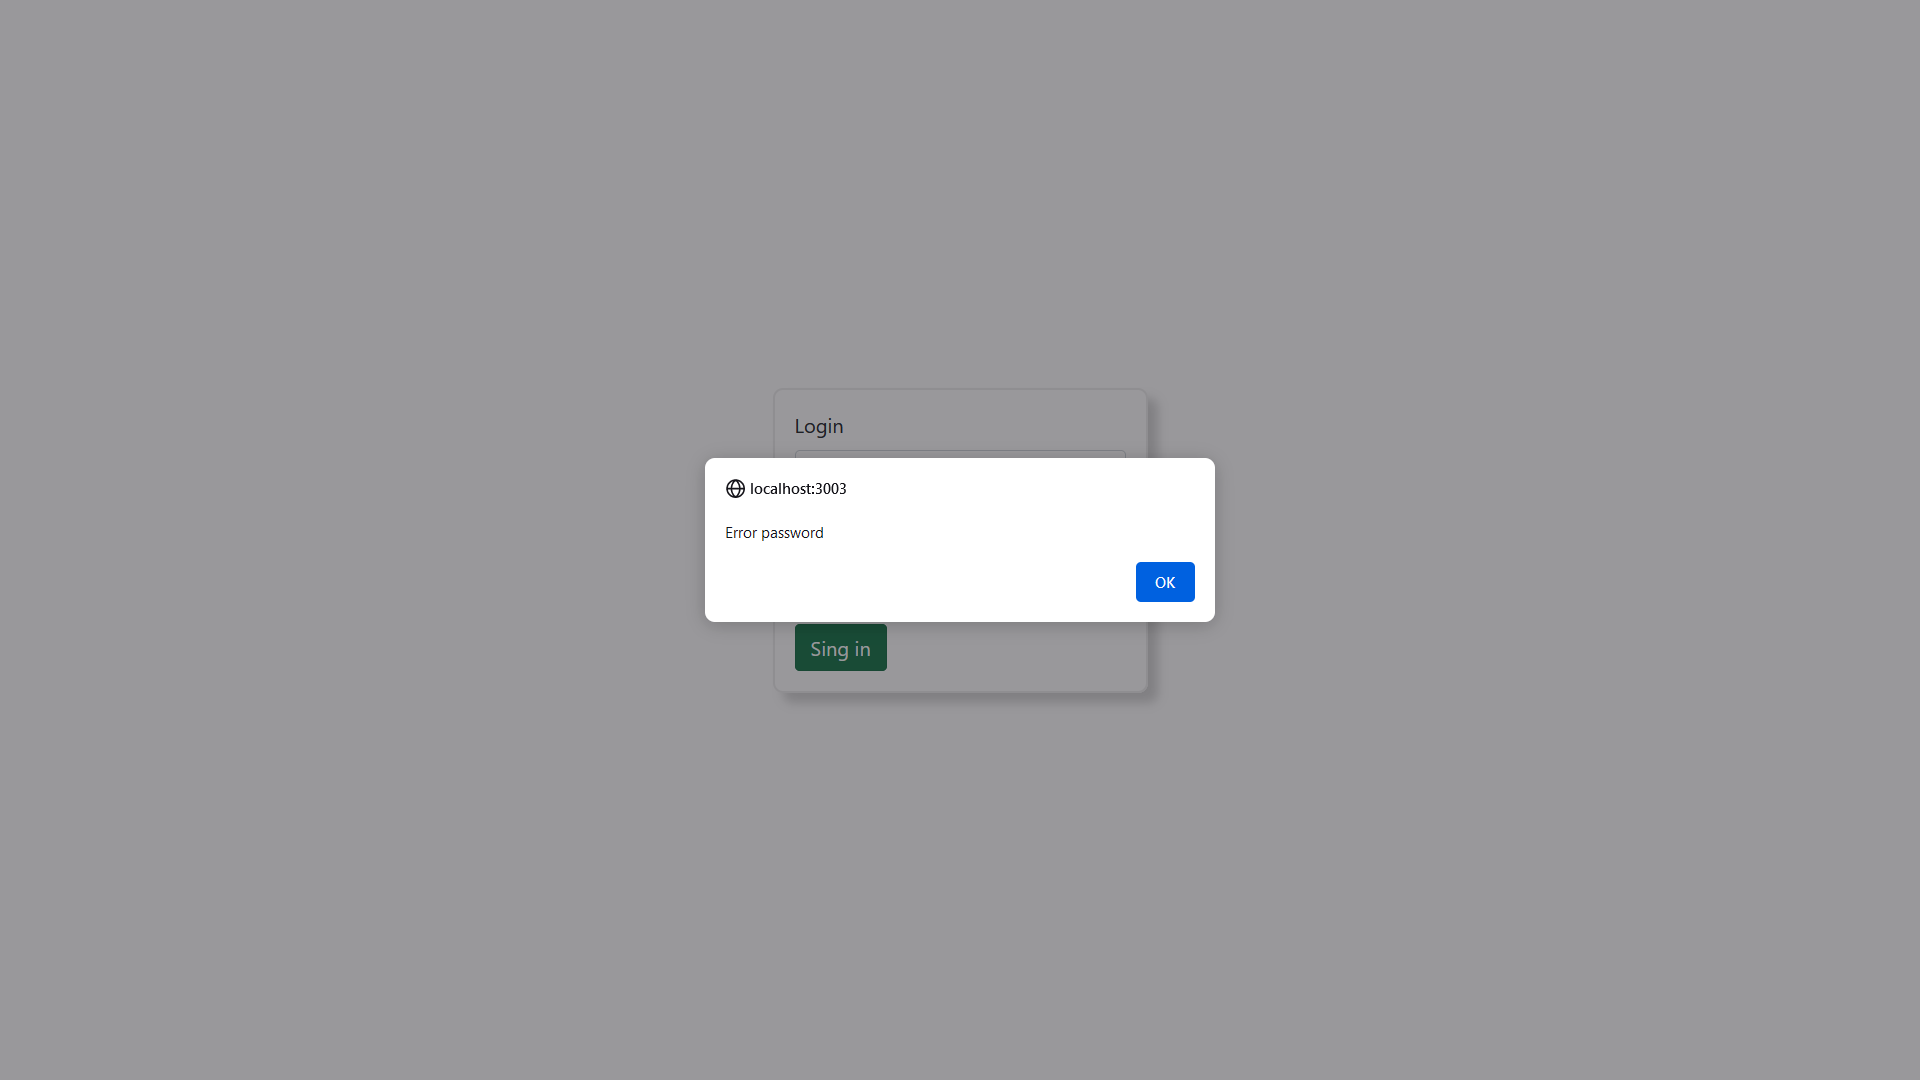
\includegraphics[width=\linewidth]
            {_assets/gpi_pz_auth_error_password.png}
        \caption{Сообщение об неверном пароле}
        \label{fig:gpi_pz_auth_error_password}
    \end{minipage}
\end{figure}

% = = = = = = = = = = = = = = = = = = = = = = = = = = = = = = = =

\subparagraph{Тестируемая задача:} <<Авторизация в панели администратора с верным вводом данных: логин существет и хэш пароля подходит>>

\textit{Ожидаемый результат}: администратор авторизуется - сервер отправит результат об успехе,
браузер перенаправится в админ панель.

\textit{Полученный результат}: администратор авторизовался, браузер перенаправил в админ панель.

\textit{Выводы по тесту}:
Скриншот страницы, на которую перенаправился администратор после успешной авторизации, на
\textbf{рис.~\ref{fig:gpi_pz_adminpanel} (стр.~\pageref{fig:gpi_pz_adminpanel})}.

\begin{figure}[!htb]
    \centering
    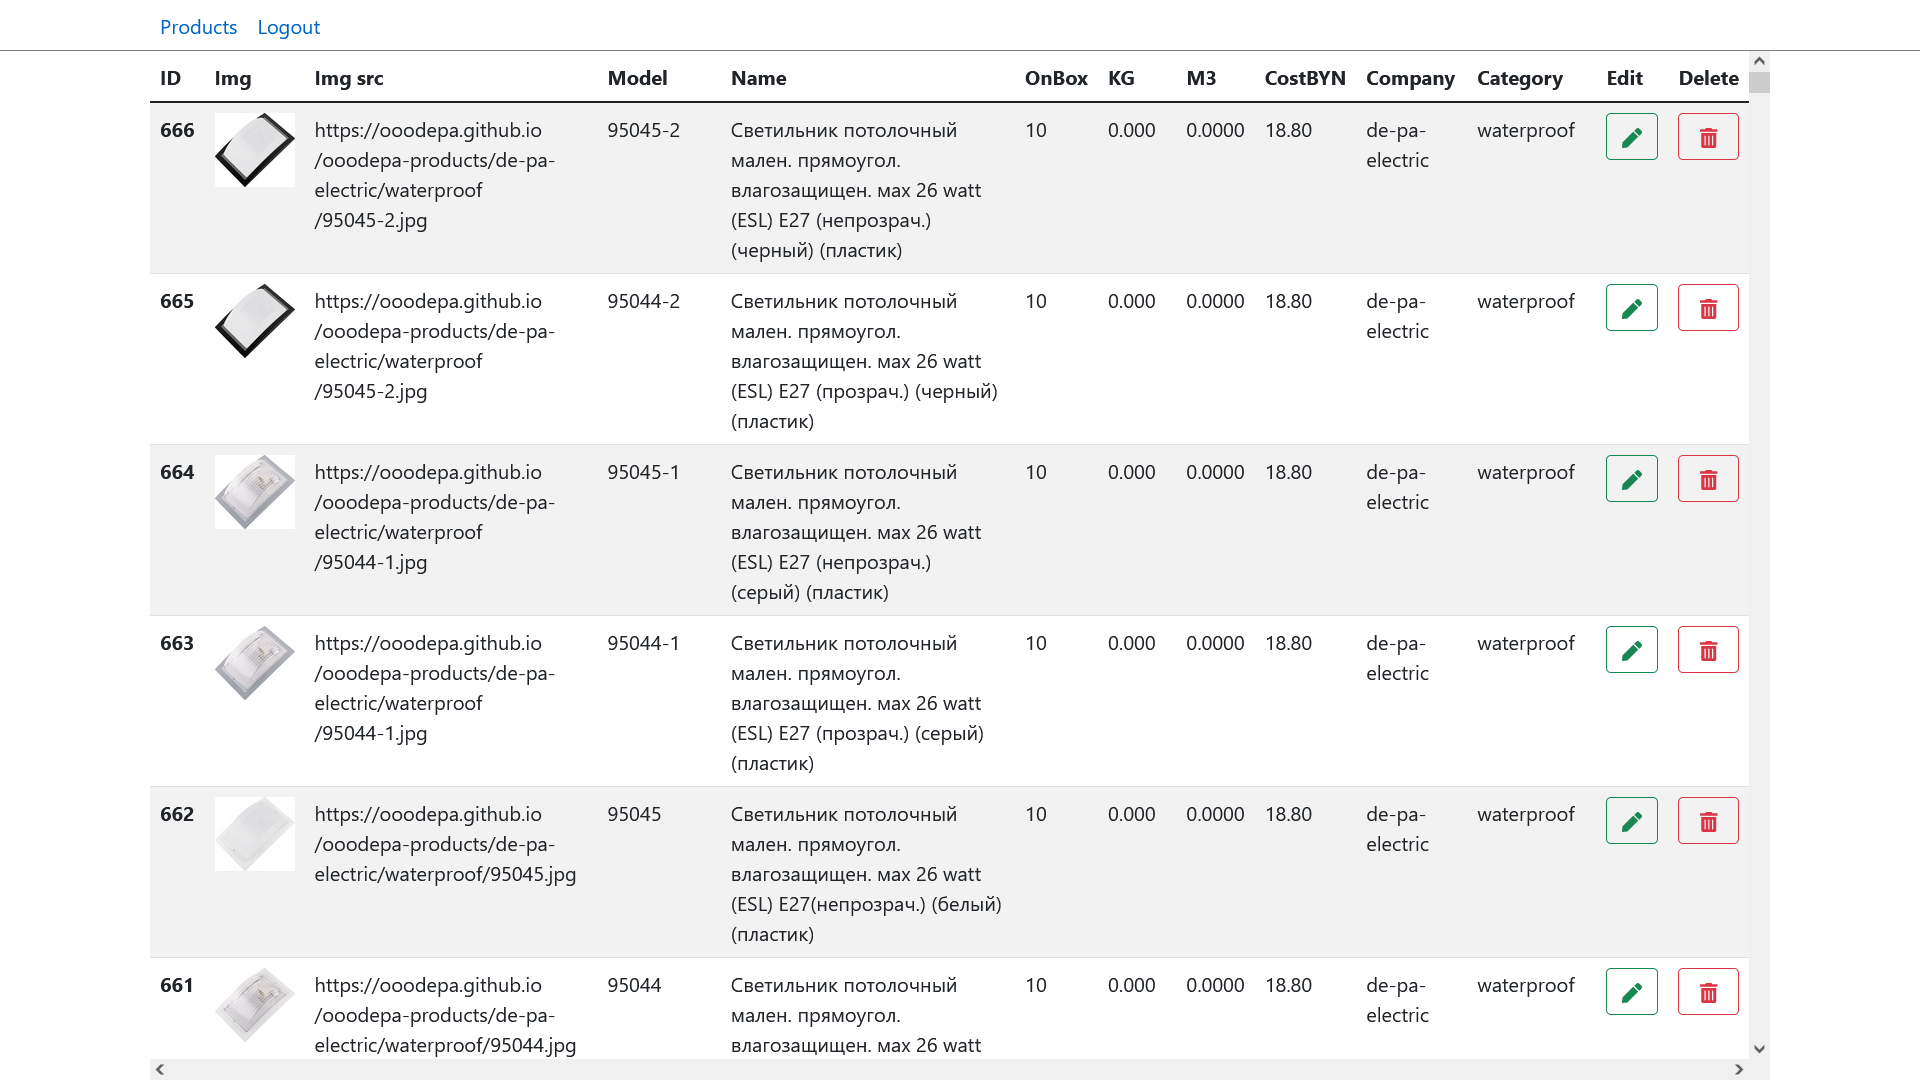
\includegraphics[width=12cm]
        {_assets/gpi_pz_not_empty_table.png}
    \caption{Таблица продуктов после открытия файла}
    \label{fig:gpi_pz_adminpanel}
\end{figure}

% = = = = = = = = = = = = = = = = = = = = = = = = = = = = = = = =

\subparagraph{Тестируемая задача:} <<Открытие текстового файла не JSON формата>>

\textit{Ожидаемый результат}: файл загрузится в браузер, браузер сообщит об ошибке формата файла.

\textit{Полученный результат}: файл загрузился в браузер, браузер сообщил об ошибке формата файла.

\textit{Выводы по тесту}:
Скриншот таблицы после открытия файла на
\textbf{рис.~\ref{fig:gpi_pz_error_open_file} (стр.~\pageref{fig:gpi_pz_error_open_file})}.

\begin{figure}[!htb]
    \centering
    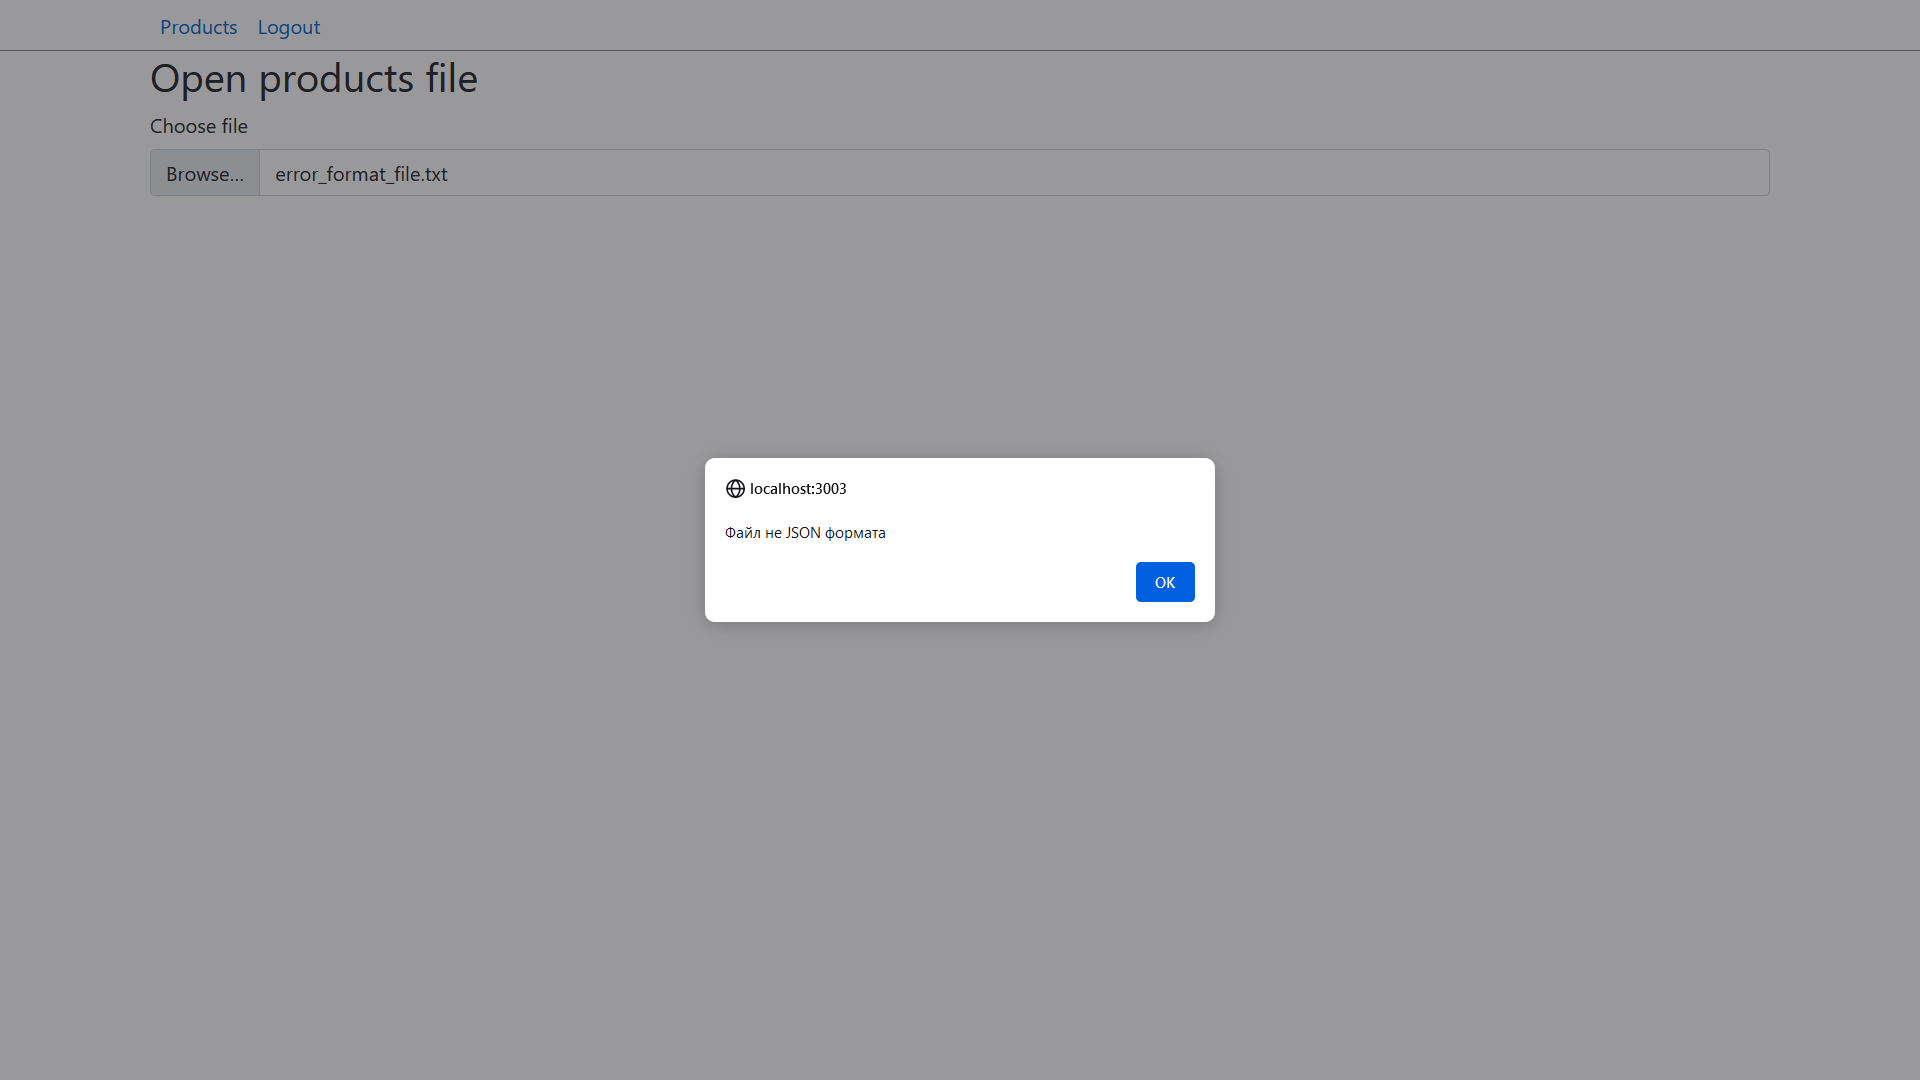
\includegraphics[width=10cm]
        {_assets/gpi_pz_error_open_file.png}
    \caption{Сообщение об не верном текстовом файле (не JSON)}
    \label{fig:gpi_pz_error_open_file}
\end{figure}

% = = = = = = = = = = = = = = = = = = = = = = = = = = = = = = = =

\newpage

\subparagraph{Тестируемая задача:} <<Открытие текстового файла в виде массива структур (JSON)>>

\textit{Ожидаемый результат}: файл загрузится в браузер, браузер перенаправит файл на сервер,
сервер добавит данные в таблицу MySQL и данные можно увидеть в таблице.

\textit{Полученный результат}: файл загрузился в браузер, браузер сообщил об добавленных данных.
На странице таблицы можно увидеть добавленные данные.

\textit{Выводы по тесту}:\\
Скриншот таблицы продуктов до открытия файла на
\textbf{рис.~\ref{fig:gpi_pz_empty_table} (стр.~\pageref{fig:gpi_pz_empty_table})}.\\
Скриншот сообщения о добавлении продуктовиз тектового файла на
\textbf{рис.~\ref{fig:gpi_pz_open_products_json} (стр.~\pageref{fig:gpi_pz_open_products_json})}.\\
Скриншот таблицы продуктов после открытия файла на
\textbf{рис.~\ref{fig:gpi_pz_not_empty_table} (стр.~\pageref{fig:gpi_pz_not_empty_table})}.

\begin{figure}[!h]
    \centering
    \begin{minipage}{0.47\textwidth}
        \centering
        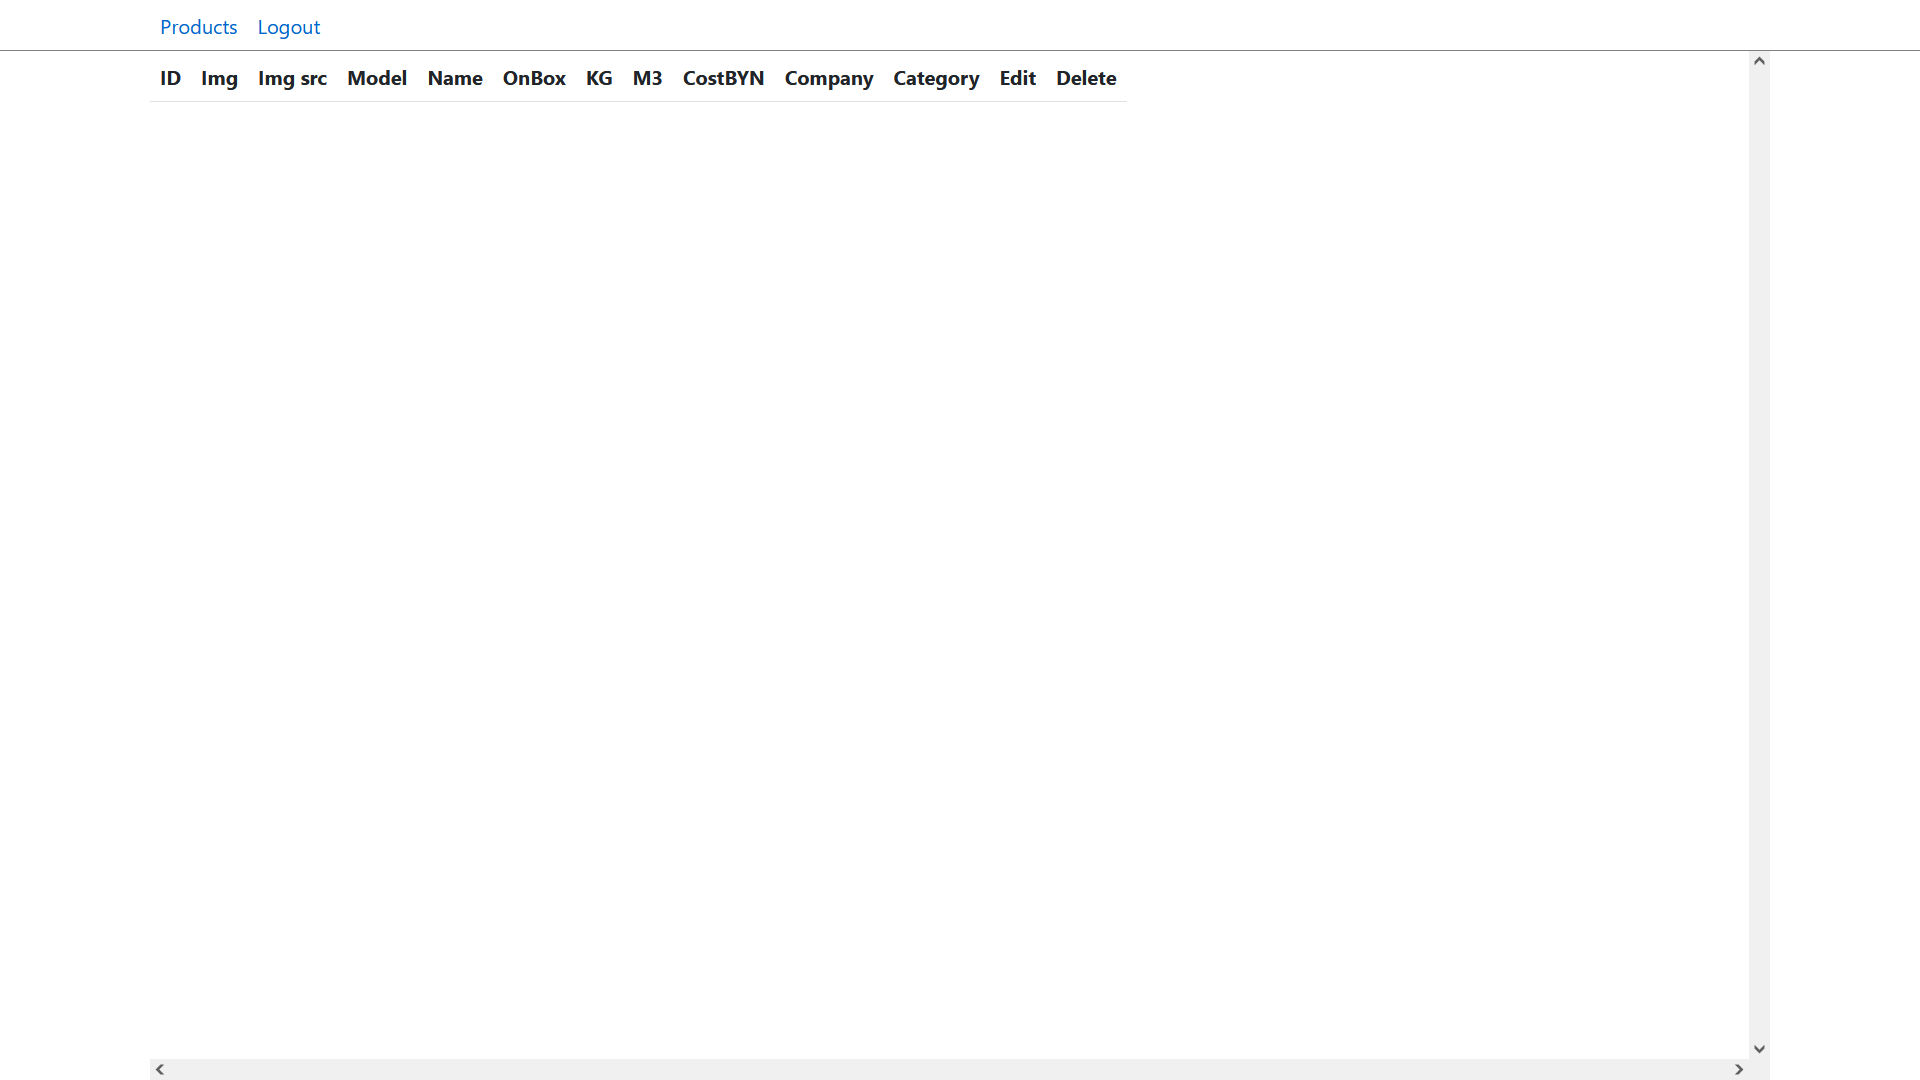
\includegraphics[width=\linewidth]
            {_assets/gpi_pz_empty_table.png}
        \caption{Таблица товаров до открытия файла}
        \label{fig:gpi_pz_empty_table}
    \end{minipage}
    \begin{minipage}{0.47\textwidth}
        \centering
        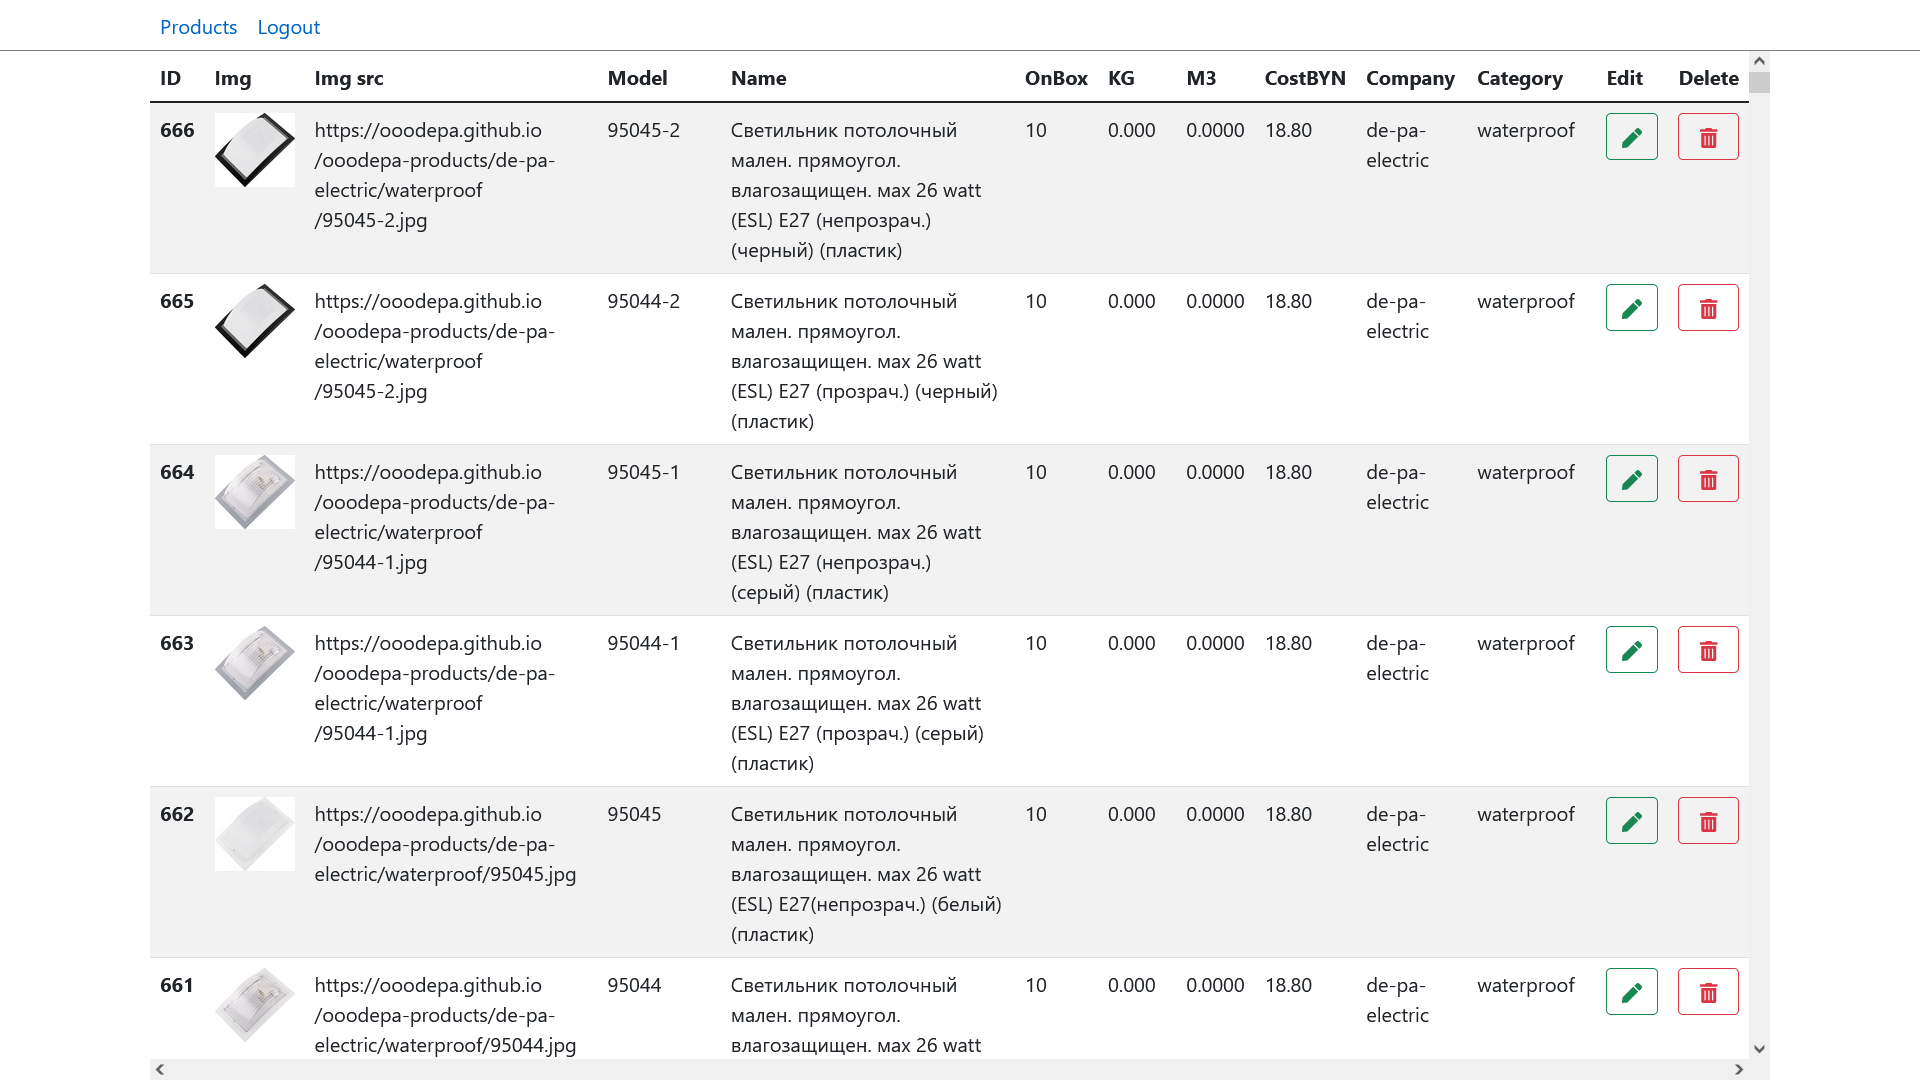
\includegraphics[width=\linewidth]
            {_assets/gpi_pz_not_empty_table.png}
        \caption{Таблица продуктов после открытия файла}
        \label{fig:gpi_pz_not_empty_table}
    \end{minipage}
\end{figure}

\begin{figure}[!htbp]
    \centering
    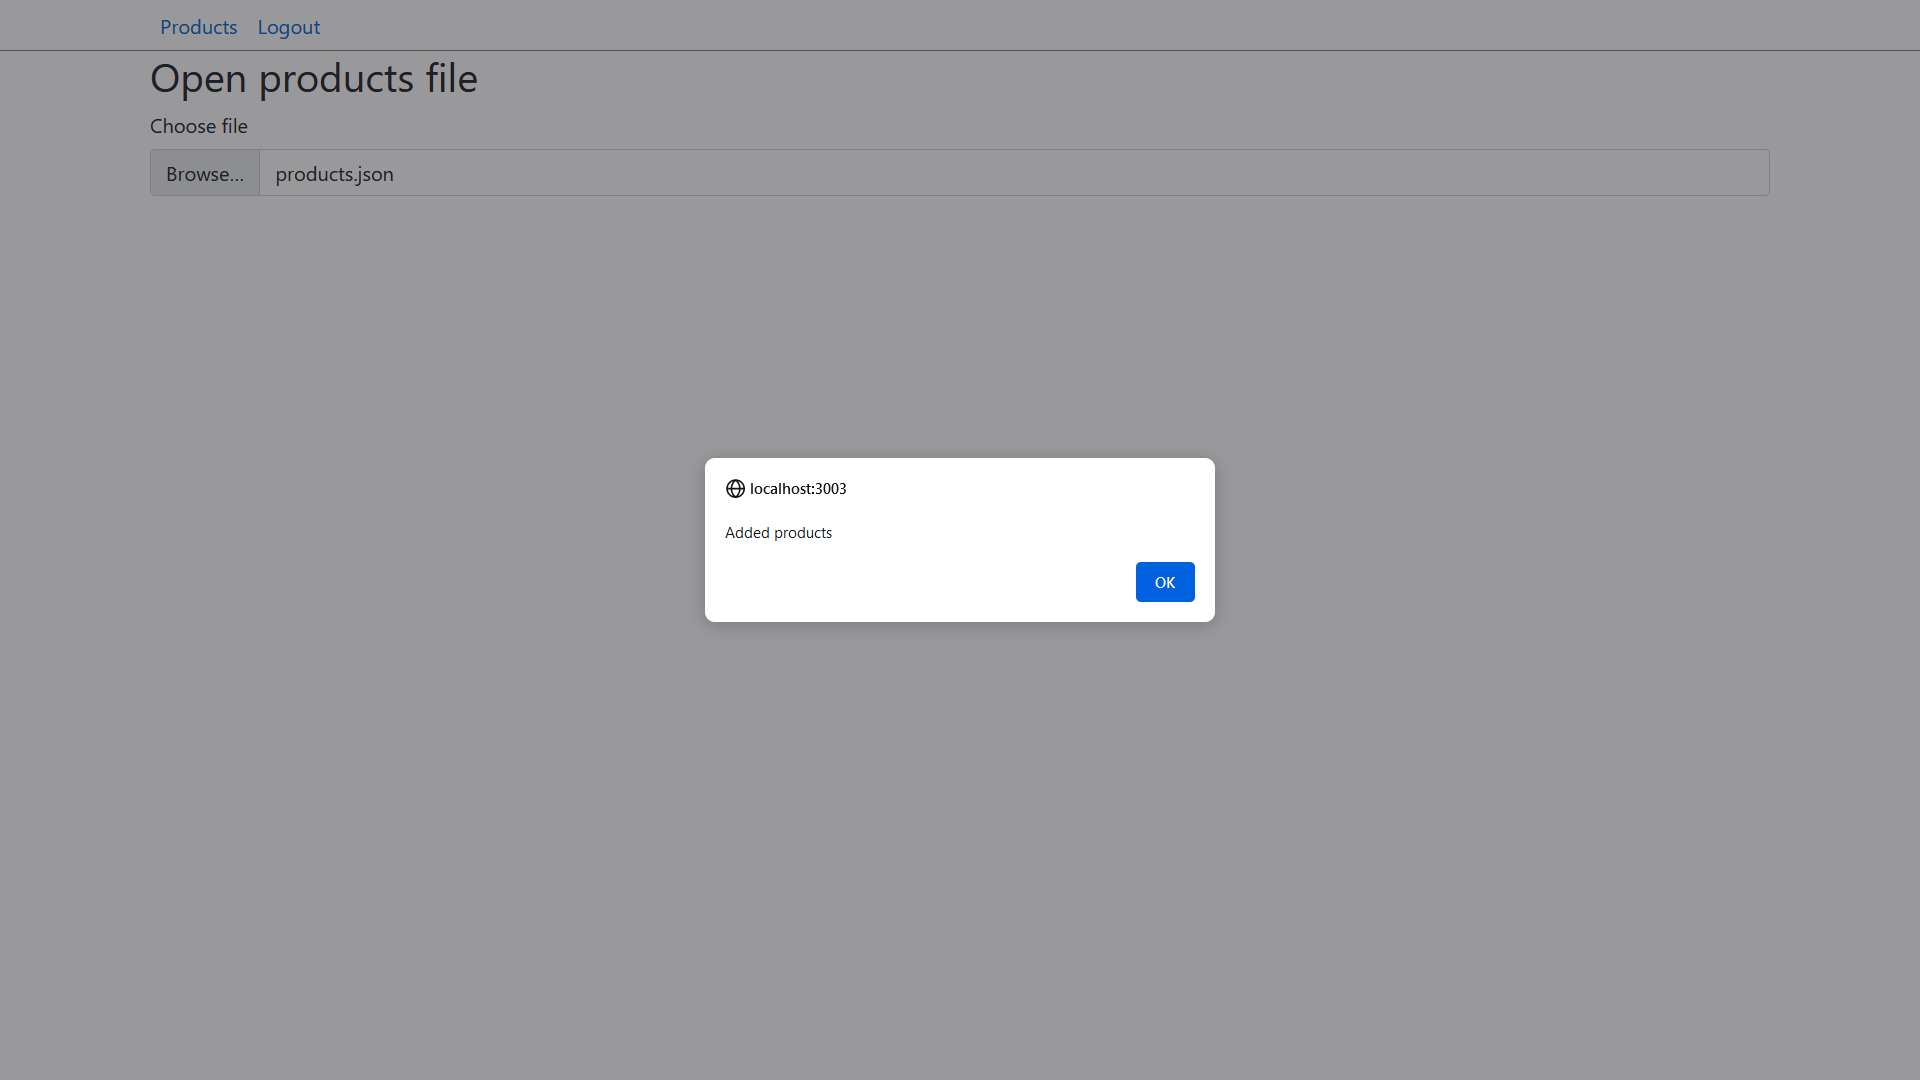
\includegraphics[width=12cm]
        {_assets/gpi_pz_open_products_json.png}
    \caption{Сообщение об добавлении продуктов из текстового файла (JSON)}
    \label{fig:gpi_pz_open_products_json}
\end{figure}

% = = = = = = = = = = = = = = = = = = = = = = = = = = = = = = = =

\newpage

\subparagraph{Тестируемая задача:} <<Просмотр таблицы продуктов>>

\textit{Ожидаемый результат}: выведится таблица продуктов.

\textit{Полученный результат}: вывелась таблица продуктов.

\textit{Выводы по тесту}:
Скриншот таблицы продуктов на
\textbf{рис.~\ref{fig:gpi_pz_products_table} (стр.~\pageref{fig:gpi_pz_products_table})}.

\begin{figure}[!htbp]
    \centering
    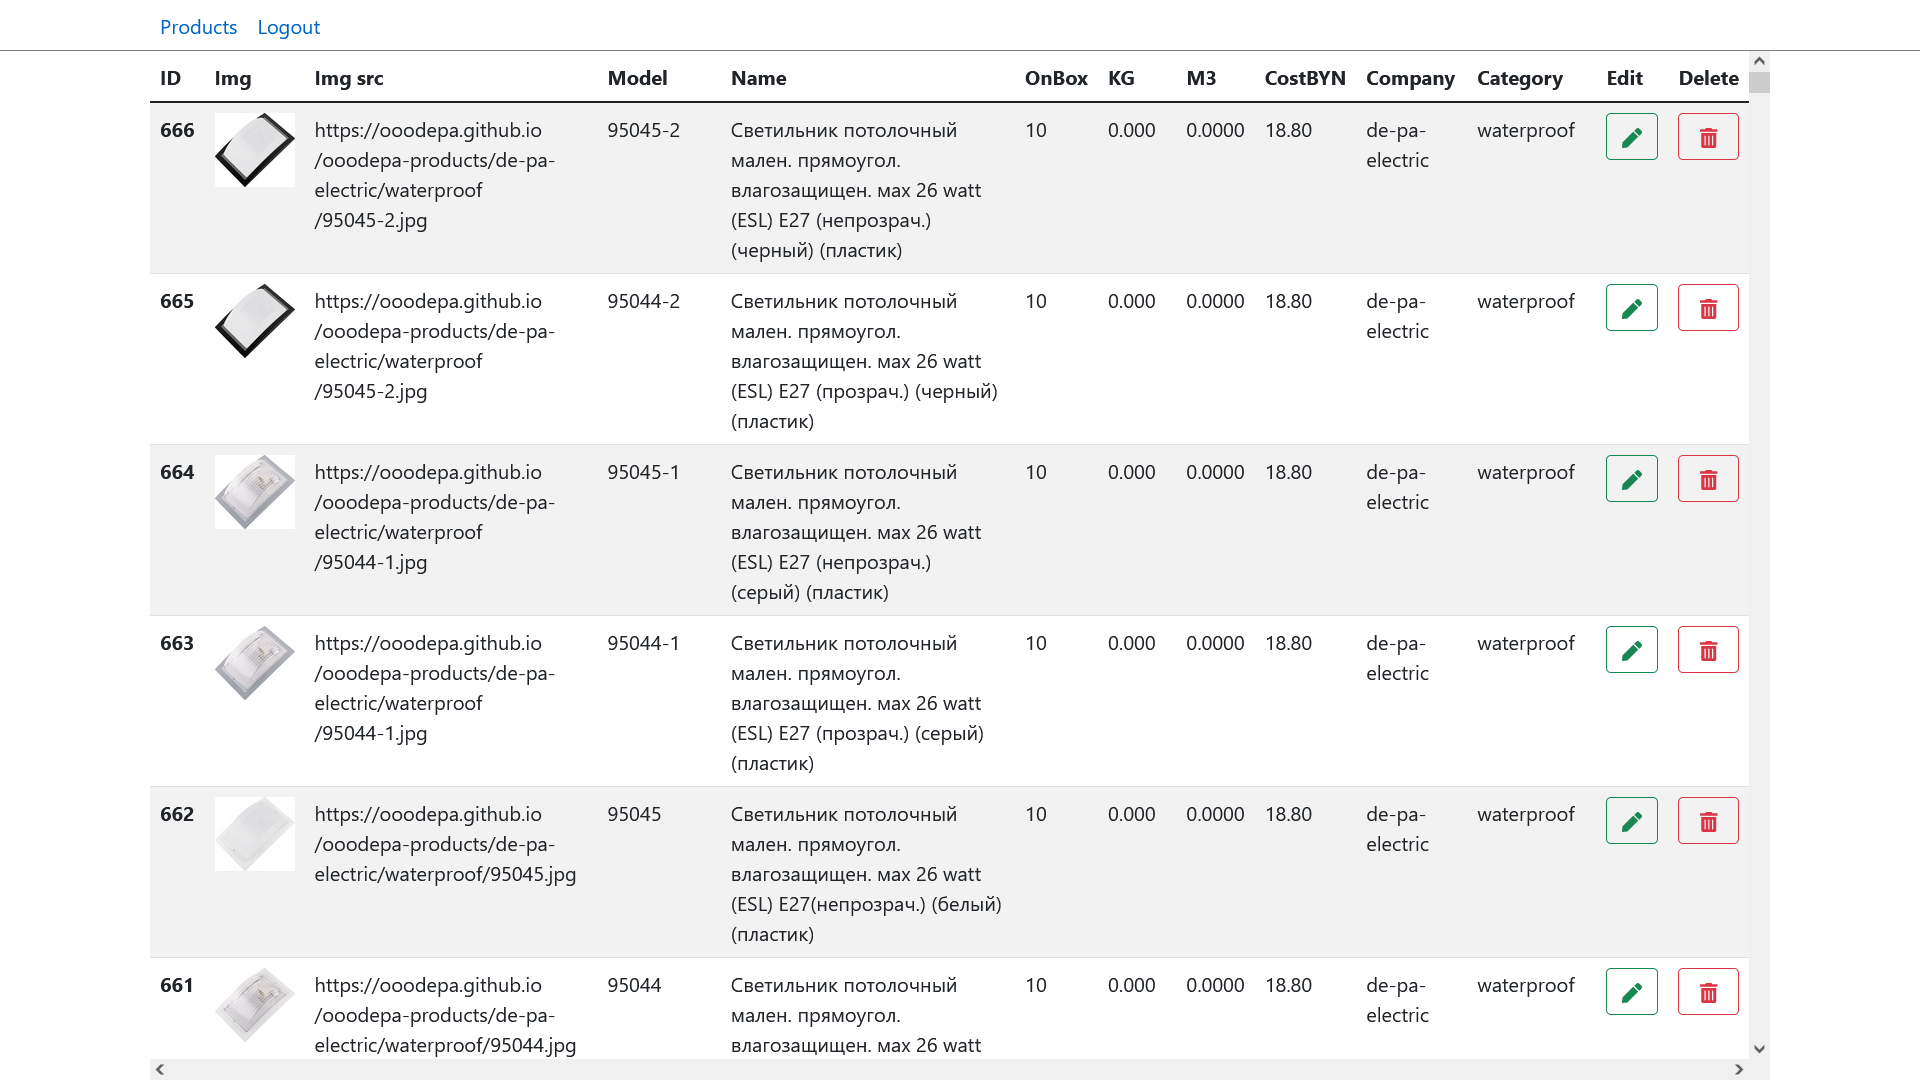
\includegraphics[width=12cm]
        {_assets/gpi_pz_not_empty_table.png}
    \caption{Таблица продуктов}
    \label{fig:gpi_pz_products_table}
\end{figure}

% = = = = = = = = = = = = = = = = = = = = = = = = = = = = = = = =

\subparagraph{Тестируемая задача:} <<Добавление нового продукта>>

\textit{Ожидаемый результат}: добавится новый продукт в БД. Данные можно увидеть в таблице продуктов.

\textit{Полученный результат}: получили сообщение о добавлении продукта. В таблице продуктов новые данные.

\textit{Выводы по тесту}: 
Скриншот соббщения о добавлении продукта на
\textbf{рис.~\ref{fig:gpi_pz_add_product} (стр.~\pageref{fig:gpi_pz_add_product})}.

\begin{figure}[!htb]
    \centering
    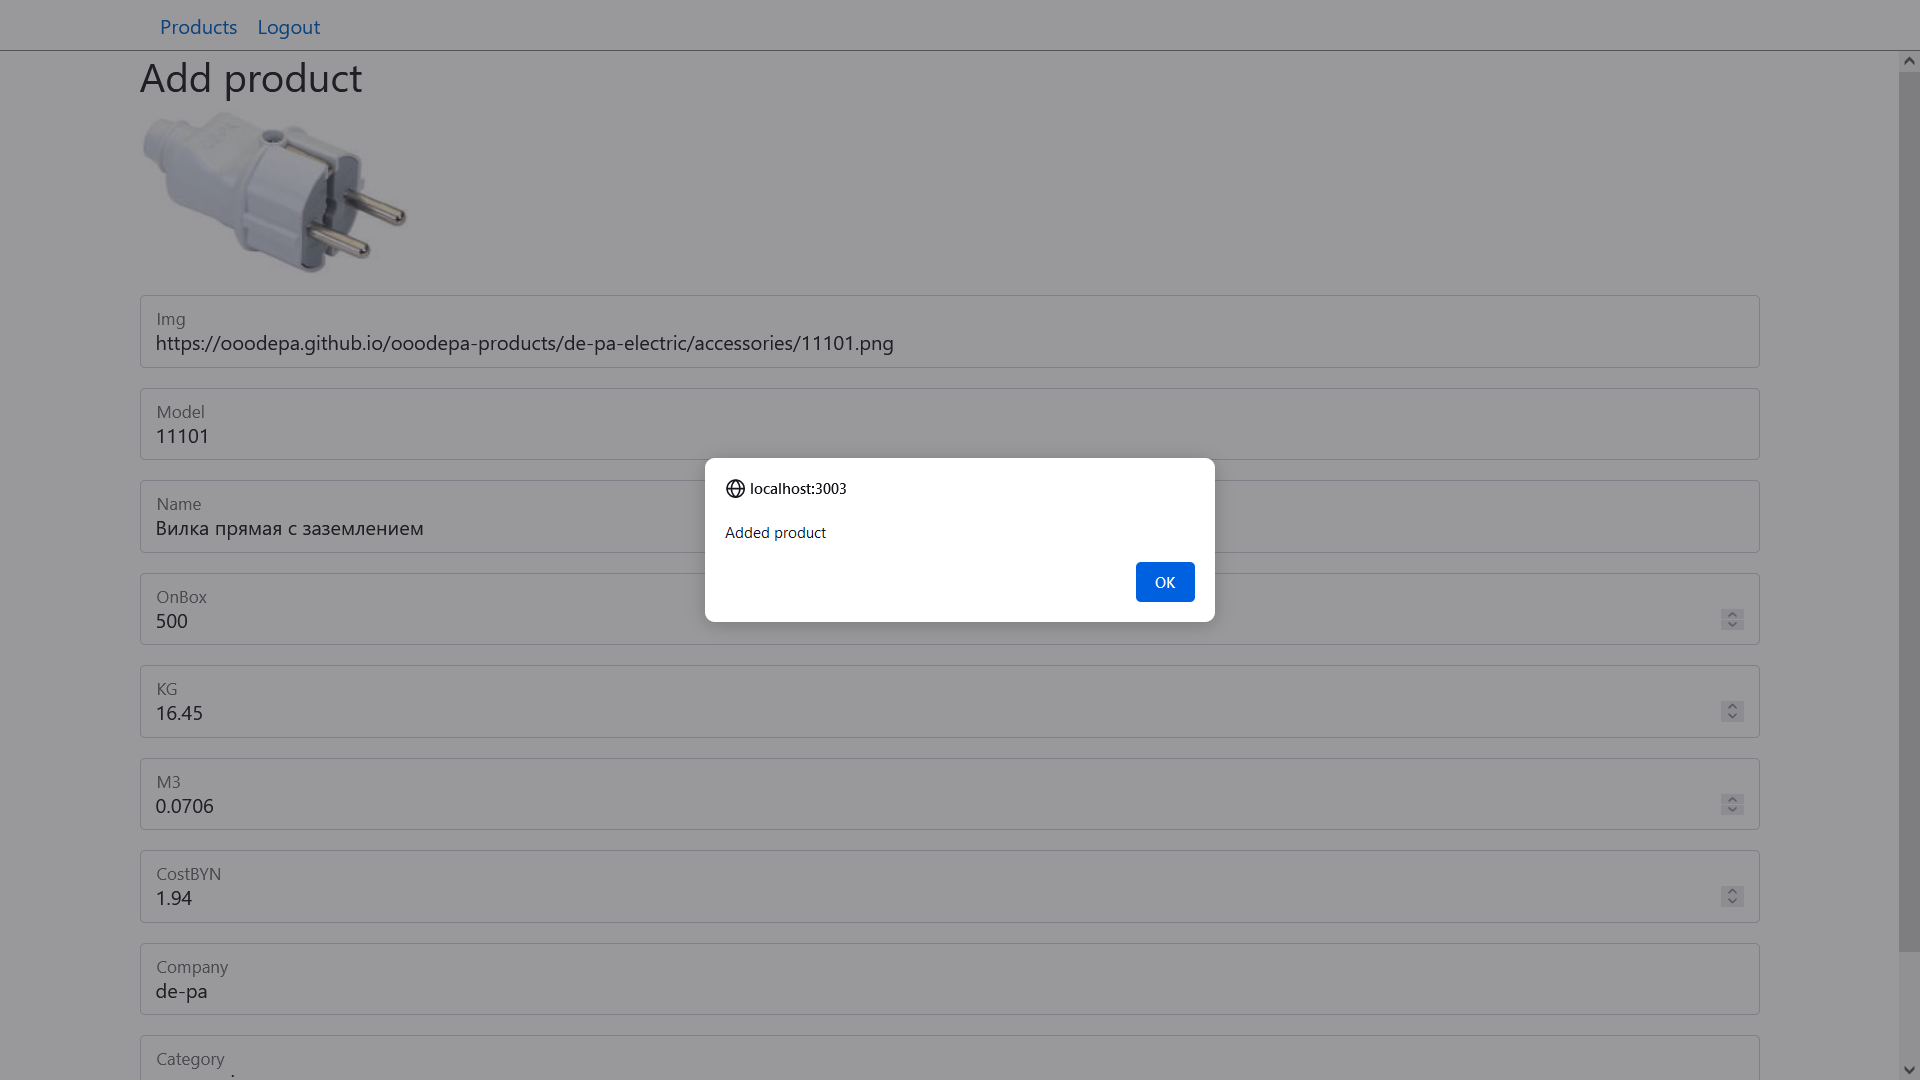
\includegraphics[width=12cm]
        {_assets/gpi_pz_add_product.png}
    \caption{Сообщение о добавлении продукта}
    \label{fig:gpi_pz_add_product}
\end{figure}

% = = = = = = = = = = = = = = = = = = = = = = = = = = = = = = = =

\subparagraph{Тестируемая задача:} <<Удаление продукта>>

\textit{Ожидаемый результат}: с таблицы удалится продукт.

\textit{Полученный результат}: продукт удалился с таблицы.

\textit{Выводы по тесту}: 
Скриншот сообщения об удалении продукта на
\textbf{рис.~\ref{fig:gpi_pz_delete_product} (стр.~\pageref{fig:gpi_pz_delete_product})}.

\begin{figure}[!htb]
    \centering
    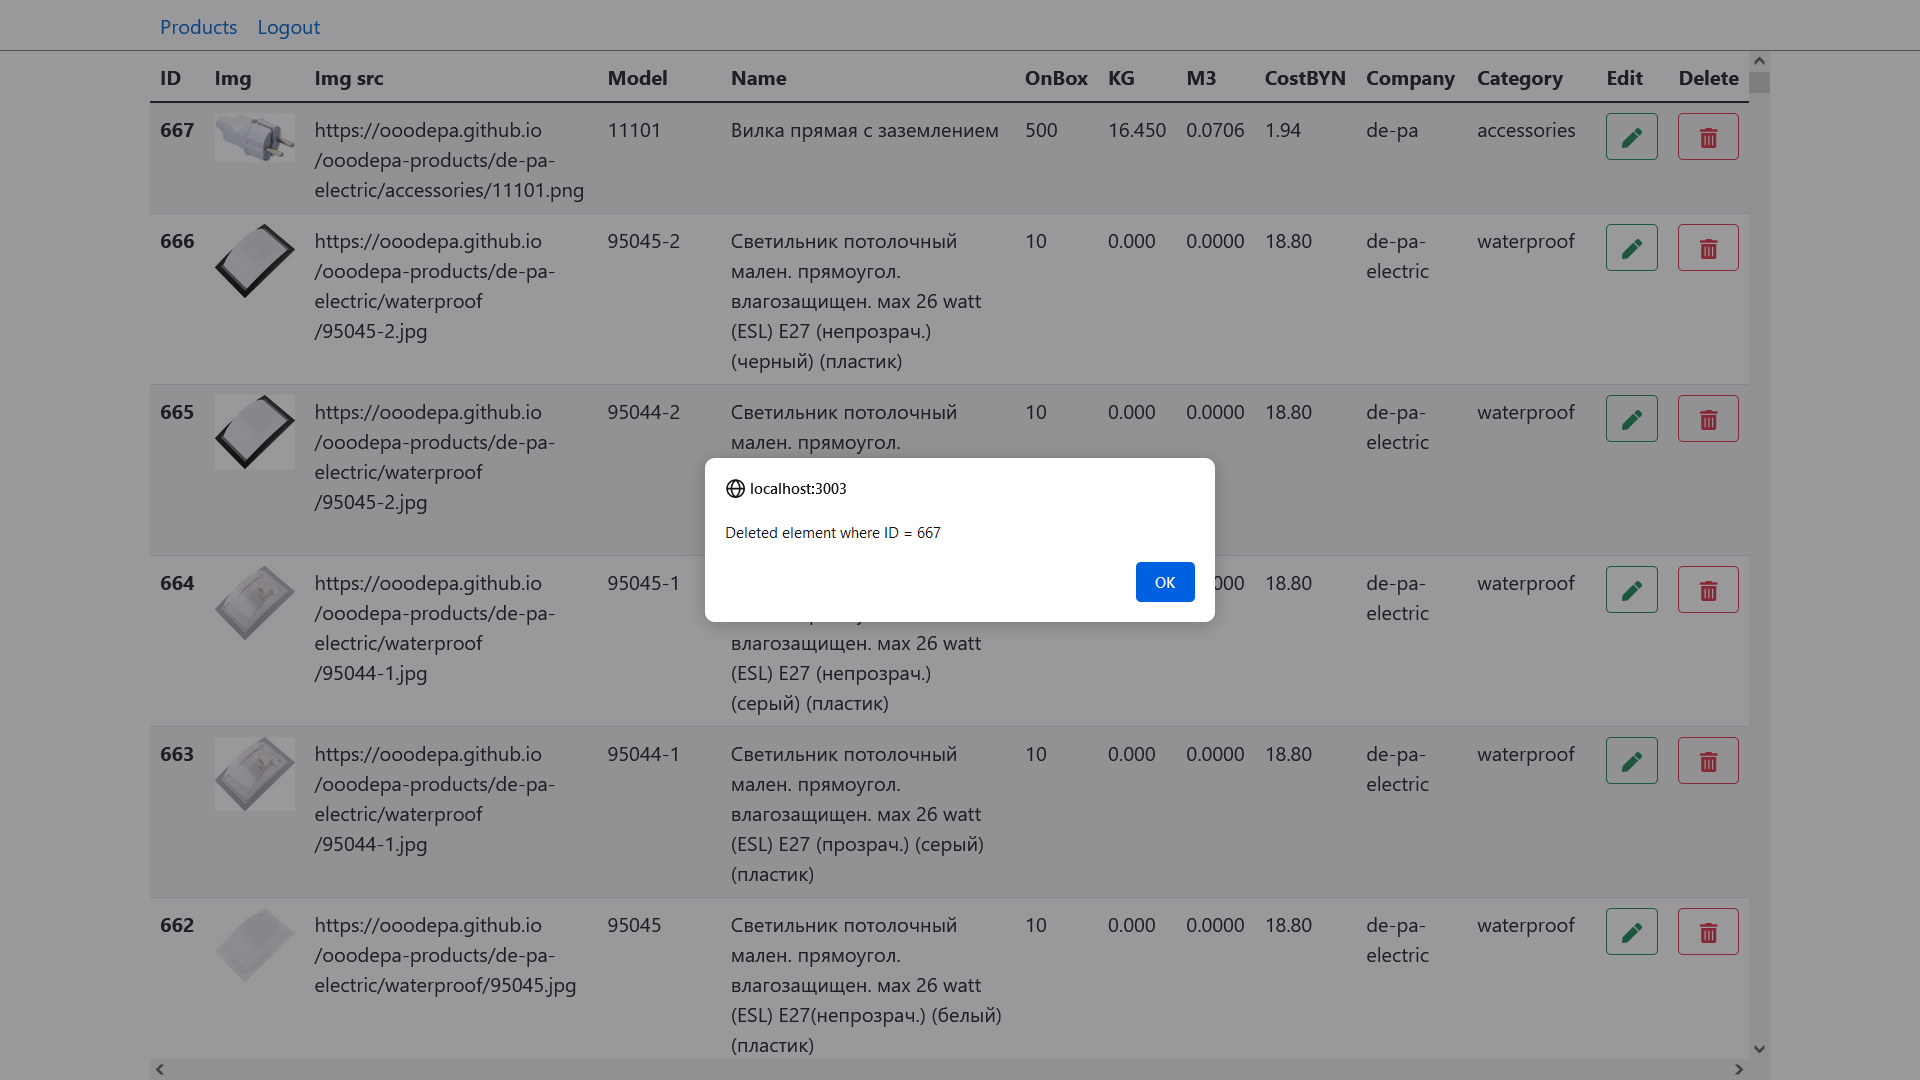
\includegraphics[width=12cm]
        {_assets/gpi_pz_delete_product.png}
    \caption{Сообщение о добавлении продукта}
    \label{fig:gpi_pz_delete_product}
\end{figure}

% = = = = = = = = = = = = = = = = = = = = = = = = = = = = = = = =

\newpage
                     % 4. Тестирование системы
    \newpage

\section*{Заключение}
\phantomsection
\addcontentsline{toc}{section}{Заключение}

В ходе выполнения данной курсовой работы усвоили и закрепили знания о работе с клиент-серверной архитектурой:
создание клиенкой части, создание серверной части.

Были разработаны различные виды проектов:

\begin{itemize}
    \item проект сервера, который возвращает JSON данные при URL запросе;
    \item виртуальная машина с баззой данных;
    \item веб-сайт с панелью администратора;
    \item веб-сайт пользователя с корзиной товаров.
\end{itemize}
	
В итоге была разработана программа,
позволяющая добавлять, удалять редактировать товары, которые выводятся на сайт пользователю.

Данная программа может быть полезна различным организациям,
которым необходимо выводить товары на сайт.

Так как большинство СНГ компаний для учёта товаров на складах (занесения записей с накладных) используют
1C Предприятие, то продолжением это проекта можно поставить цель следующую: 
разработать отчёт или функцию в 1C Конфигураторе, который/которая будет сохранять в файл JSON формат.
Раз в день загружать количество товаров на сервер.  

\newpage
                          % Заключение
    \newpage

\section*{СПИСОК ИСПОЛЬЗОВАННЫХ ИСТОЧНИКОВ}
\addcontentsline{toc}{section}{СПИСОК ИСПОЛЬЗОВАННЫХ ИСТОЧНИКОВ}

\begin{enumerate}
    \item Получение GET и POST запросов на Node.js \\
    \url{https://youtu.be/YMJDUHUccvA}

    \item Подключение к базе данных MySQL в Node.js \\
    \url{https://youtu.be/YhuozY-qplI}

    \item Модули Node.js, require \\
    \url{https://youtu.be/1PkarXC-9TQ}
\end{enumerate}
                          % СПИСОК ИСПОЛЬЗОВАННЫХ ИСТОЧНИКОВ
\end{document}
